                
% ----------------------------------------------------------------------
%                   LATEX TEMPLATE FOR PhD THESIS
% ----------------------------------------------------------------------

% based on Harish Bhanderi's PhD/MPhil template, then Uni Cambridge
% http://www-h.eng.cam.ac.uk/help/tpl/textprocessing/ThesisStyle/
% corrected and extended in 2007 by Jakob Suckale, then MPI-CBG PhD programme
% and made available through OpenWetWare.org - the free biology wiki


%: Style file for Latex
% Most style definitions are in the external file PhDthesisPSnPDF.
% In this template package, it can be found in ./Latex/Classes/
\documentclass[twoside,11pt,table,xcdraw]{Latex/Classes/PhDthesisPSnPDF}

\newcommand{\ana}[2][inline]{\color{red} [AI]: #2\color{black}}

\usepackage[utf8]{inputenc}
\usepackage[english]{babel}
\usepackage{lipsum}  
\usepackage{multirow}
\usepackage{xcolor}
\usepackage{rotating}
\usepackage{caption}
\usepackage{lscape}
\usepackage{hvfloat}
%\usepackage[table,xcdraw]{xcolor}
\usepackage{multirow}
\usepackage{balance}

\usepackage{listings}
\def\dollar{\$}
\lstset{mathescape=true}
\lstset{%
	basicstyle=\scriptsize\ttfamily,%
	basewidth=.5em,%
	captionpos=b,
	frame=single,
	tabsize=4,
	numbers=left}%
\lstset{
	escapechar={(@}{^)}
}
\lstset{
   literate=
        {í}{{\'i}}1
        {ñ}{{\~n}}1
}
%% -- Listings

\colorlet{punct}{red!60!black}
\definecolor{background}{HTML}{EEEEEE}
\definecolor{delim}{RGB}{20,105,176}
\colorlet{numb}{magenta!60!black}
\definecolor{burgundy}{rgb}{0.5, 0.0, 0.13}
\lstdefinelanguage{json}{
	keywords=[1]{},
	keywordstyle=[1]\color{teal}\bfseries,
	keywords=[2]{resource_rules, id, datasource_ids, subject, properties, predicate, object, is_literal, link_rules, condition, source, target},	% types; money and time units
	keywordstyle=[2]\color{burgundy}\bfseries,
    basicstyle=\footnotesize\ttfamily,
    numbers=left,
    numberstyle=\scriptsize,
    stepnumber=1,
    numbersep=8pt,
    showstringspaces=false,
    identifierstyle=\color{black},
    breaklines=true,
    backgroundcolor=\color{verylightgray},
    literate=
     *{:}{{{\color{black}{:}}}}{1}
      {\$}{{{\color{punct}{\$}}}}{1}
      {,}{{{\color{red}{,}}}}{1}
      {\{}{{{\color{red}{\{}}}}{1}
      {\}}{{{\color{red}{\}}}}}{1}
      {[}{{{\color{red}{[}}}}{1}
      {]}{{{\color{red}{]}}}}{1},
}
\definecolor{bittersweet}{rgb}{1.0, 0.44, 0.37}
\lstdefinelanguage{Shex}{
	keywords=[1]{},
	keywordstyle=[1]\color{teal}\bfseries,
	keywords=[2]{SOURCE, ITERATOR, FIELD},	% types; money and time units
	keywordstyle=[2]\color{bittersweet}\bfseries,
	keywords=[3]{c_city, cities_rdb, coord_json, it_cities, population, year, zipcode, it_coord, lat, long, loc_city, long},
	keywordstyle=[3]\color{teal}\bfseries,
	identifierstyle=\color{black},
	sensitive=true,
	comment=[l]{//},
	morecomment=[s]{/*}{*/},
	commentstyle=\color{black}\ttfamily,
	stringstyle=\color{fulvous}\bfseries,
	morestring=[b]',
	morestring=[b]",
	literate=
     *{\{}{{{\color{bittersweet}{\{}}}}{1}
      {\}}{{{\color{bittersweet}{\}}}}}{1}
      {<}{{{\color{bittersweet}{<}}}}{1}
      {>}{{{\color{bittersweet}{>}}}}{1},
}

\lstdefinelanguage{yarrrml}{
	keywords=[1]{},
	keywordstyle=[1]\color{teal}\bfseries,
	keywords=[2]{mappings, sources, s, po, function, parameters, value, parameter},	% types; money and time units
	keywordstyle=[2]\color{violet}\bfseries,
	keywords=[3]{Locations, Cities},
	keywordstyle=[3]\color{teal}\bfseries,	
	keywords=[4]{xsd, double, integer, boolean, decimal, string},
	keywordstyle=[4]\color{applegreen}\bfseries,
	identifierstyle=\color{black},
	sensitive=true,
	comment=[l]{//},
	morecomment=[s]{/*}{*/},
	commentstyle=\color{black}\ttfamily,
	stringstyle=\color{fulvous}\bfseries,
	morestring=[b]',
	morestring=[b]",
	literate=
     *{[}{{{\color{violet}{[}}}}{1}
      {]}{{{\color{violet}{]}}}}{1}
       {-}{{{\color{violet}\bfseries{-}}}}{1},
}

\lstdefinelanguage{sparql}{
	keywords=[1]{} % generic keywords including crypto operations
	keywordstyle=[1]\color{blue}\bfseries,
	keywords=[2]{},	% types; money and time units
	keywordstyle=[2]\color{teal}\bfseries,
	keywords=[3]{block, blockhash, coinbase, difficulty, gaslimit, number, timestamp, msg, data, gas, sender, sig, value, now, tx, gasprice, origin},	% environment variables
	keywordstyle=[3]\color{violet}\bfseries,
	keywords=[4]{xsd, double, integer, boolean, decimal, string},
	keywordstyle=[4]\color{applegreen}\bfseries,
	keywordstyle=[5]\color{iris}\bfseries,
	keywords=[5]{GENERATE, REPLACE, WHERE, FILTER},
	identifierstyle=\color{black},
	sensitive=false,
	comment=[l]{//},
	morecomment=[s]{/*}{*/},
	commentstyle=\color{gray}\ttfamily,
	stringstyle=\color{fulvous}\bfseries,
	morestring=[b]',
	morestring=[b]"
}

\lstdefinelanguage{concm}{
	keywords=[1]{} % generic keywords including crypto operations
	keywordstyle=[1]\color{blue}\bfseries,
	keywords=[2]{Locations, Cities, Sources, Rules},	% types; money and time units
	keywordstyle=[2]\color{violet}\bfseries,
	keywords=[3]{cm, dcat, expression, hasField, hasDataSource, mediaType, SourceFrame, accessService, hasProtocol, endpointURL, hasSecurityScheme, DataField, field, hasNestedFrame, ReferenceNodeMap, hasEvaluableExpression, hasFunctionName, hasInput, subject, predicate, hasFrame, constantValue, Literal, object, FunctionExpression, functionName, hasBooleanCondition, hasDatatype, source, target, property, LinkingExpression, ConditionalStatementMap, SynchronousSource, StatementMap, JoinCombination, datatype, language, combinesFrame, joinsBy, ListMap, hasLanguage},	% environment variables
	keywordstyle=[3]\color{steelblue}\bfseries,
	keywords=[4]{xsd, double, integer, boolean, decimal, string, time},
	keywordstyle=[4]\color{applegreen}\bfseries,
	identifierstyle=\color{black},
	sensitive=false,
	comment=[l]{//},
	morecomment=[s]{/*}{*/},
	commentstyle=\color{gray}\ttfamily,
	stringstyle=\color{fulvous}\bfseries,
	morestring=[b]',
	morestring=[b]",
}

\definecolor{verylightgray}{rgb}{.97,.97,.97}
\definecolor{applegreen}{rgb}{0.55, 0.71, 0.0}
\definecolor{iris}{rgb}{0.35, 0.31, 0.81}
\definecolor{richelectricblue}{rgb}{0.03, 0.57, 0.82}
\definecolor{shamrockgreen}{rgb}{0.0, 0.62, 0.38}
\definecolor{fulvous}{rgb}{0.86, 0.52, 0.0}
\definecolor{steelblue}{rgb}{0.27, 0.51, 0.71}

\lstdefinelanguage{Solidity}{
	keywords=[1]{} % generic keywords including crypto operations
	keywordstyle=[1]\color{blue}\bfseries,
	keywords=[2]{CitiesSource, LocationSource, Locations, Cities},	% types; money and time units
	keywordstyle=[2]\color{richelectricblue}\bfseries,
	keywords=[3]{rr, xrr, logicalSource, subjectMap, predicateObjectMap, tableName, predicate, objectMap, template, reference, class, datatype, TriplesMap, LogicalTable},	% environment variables
	keywordstyle=[3]\color{shamrockgreen}\bfseries,
	keywords=[4]{xsd, double, integer, boolean, decimal, string, time},
	keywordstyle=[4]\color{applegreen}\bfseries,
	identifierstyle=\color{black},
	sensitive=false,
	comment=[l]{//},
	morecomment=[s]{/*}{*/},
	commentstyle=\color{gray}\ttfamily,
	stringstyle=\color{fulvous}\bfseries,
	morestring=[b]',
	morestring=[b]",
}

\lstset{
	language=Solidity,
	backgroundcolor=\color{verylightgray},
	extendedchars=true,
	basicstyle=\footnotesize\ttfamily,
	showstringspaces=false,
	showspaces=false,
	numbers=left,
	numberstyle=\footnotesize,
	numbersep=9pt,
	tabsize=2,
	breaklines=true,
	showtabs=false,
	captionpos=b
}

%% --

\usepackage{xparse}
\newcounter{captionedlistingcounter}
\NewDocumentEnvironment{captionedlisting}{mmm}{
	\refstepcounter{captionedlistingcounter}
	% commented out the figure part bc we don't need it and they couldn't be used in minipages
	% not sure if this is actually different from using the default listing captions/labels now
	%\begin{figure}[#3]
	{\centering\label{#1}}

}{

	\vspace{0.5\baselineskip}
	Listing \thecaptionedlistingcounter: #2
	\\%\end{figure}
}

\usepackage[capitalize,nameinlink]{cleveref}
\crefname{line}{line}{lines}
\Crefname{Line}{Line}{Lines}
\crefname{captionedlistingcounter}{Listing}{Listings}
\Crefname{captionedlistingcounter}{Listing}{Listings}
\crefformat{footnote}{#2\footnotemark[#1]#3}

%: Macro file for Latex
% Macros help you summarise frequently repeated Latex commands.
% Here, they are placed in an external file /Latex/Macros/MacroFile1.tex
% An macro that you may use frequently is the figuremacro (see introduction.tex)
%% This file contains macros that can be called up from connected TeX files
% It helps to summarise repeated code, e.g. figure insertion (see below).

% insert a centered figure with caption and description
% parameters 1:filename, 2:title, 3:description and label
\newcommand{\figuremacro}[3]{
	\begin{figure}[htbp]
		\centering
		\includegraphics[width=1\textwidth]{#1}
		\caption[#2]{\textbf{#2} - #3}
		\label{#1}
	\end{figure}
}

% insert a centered figure with caption and description AND WIDTH
% parameters 1:filename, 2:title, 3:description and label, 4: textwidth
% textwidth 1 means as text, 0.5 means half the width of the text
\newcommand{\figuremacroW}[4]{
	\begin{figure}[htbp]
		\centering
		\includegraphics[width=#4\textwidth]{#1}
		\caption[#2]{\textbf{#2} - #3}
		\label{#1}
	\end{figure}
}

% inserts a figure with wrapped around text; only suitable for NARROW figs
% o is for outside on a double paged document; others: l, r, i(inside)
% text and figure will each be half of the document width
% note: long captions often crash with adjacent content; take care
% in general: above 2 macro produce more reliable layout
\newcommand{\figuremacroN}[3]{
	\begin{wrapfigure}{o}{0.5\textwidth}
		\centering
		\includegraphics[width=0.48\textwidth]{#1}
		\caption[#2]{{\small\textbf{#2} - #3}}
		\label{#1}
	\end{wrapfigure}
}

% predefined commands by Harish
\newcommand{\PdfPsText}[2]{
  \ifpdf
     #1
  \else
     #2
  \fi
}

\newcommand{\IncludeGraphicsH}[3]{
  \PdfPsText{\includegraphics[height=#2]{#1}}{\includegraphics[bb = #3, height=#2]{#1}}
}

\newcommand{\IncludeGraphicsW}[3]{
  \PdfPsText{\includegraphics[width=#2]{#1}}{\includegraphics[bb = #3, width=#2]{#1}}
}

\newcommand{\InsertFig}[3]{
  \begin{figure}[!htbp]
    \begin{center}
      \leavevmode
      #1
      \caption{#2}
      \label{#3}
    \end{center}
  \end{figure}
}


%%% Local Variables: 
%%% mode: latex
%%% TeX-master: "~/Documents/LaTeX/CUEDThesisPSnPDF/thesis"
%%% End: 




%: ----------------------------------------------------------------------
%:                  TITLE PAGE: name, degree,..
% ----------------------------------------------------------------------
% below is to generate the title page with crest and author name

%if output to PDF then put the following in PDF header
\ifpdf  
    \pdfinfo { /Title 
               /Creator (TeX)
               /Producer (pdfTeX)
               /Author (Ana Iglesias Molina ana.iglesiasm@upm.es)
               /CreationDate (D:YYYYMMDDhhmmss)  %format D:YYYYMMDDhhmmss
               /ModDate (D:YYYYMMDDhhmm)
               /Subject (xyz)
               /Keywords () }
    \pdfcatalog { /PageMode (/UseOutlines)
                  /OpenAction (fitbh)  }
\fi

  
\title{Devising an Interoperable and Governable Environment of Mapping Languages for Knowledge Graph Construction}

% ----------------------------------------------------------------------
% The section below defines www links/email for author and institutions
% They will appear on the title page of the PDF and can be clicked
\ifpdf
 
  \author{{\hspace{7mm} Ana Iglesias Molina}}
  \supervisor{Oscar Corcho}
	%
	
%  \cityofbirth{born in XYZ} % uncomment this if your university requires this
%  % If city of birth is required, also uncomment 2 sections in PhDthesisPSnPDF
%  % Just search for the "city" and you'll find them.
%  \collegeordept{{Programa de Doctorado de Inteligencia Artificial \\ Facultad de Inform\'atica}}  
%  \university{\href{http://www.upm.es}{Universidad Polit\'ecnica de Madrid}}  
  % The crest is a graphics file of the logo of your research institution.
  % Place it in ./0_frontmatter/figures and specify the width
%  \crest{
\includegraphics[width=3cm]{escudofi.pdf}}
\crest{  
		\centering
 		\begin{tabular}{l c}
			\multirow{3}{*}{
\includegraphics[width=2cm]{0_frontmatter/figures/escudofi.pdf}} & \\
			& \textbf{Programa de Doctorado de Inteligencia Artificial} \\ 
			& \textbf{Escuela T\'ecnica Superior de Ingenieros Inform\'aticos} \\
		\end{tabular}
}
% If you are not creating a PDF then use the following. The default is PDF.
\else
  \author{YourName}
%  \cityofbirth{born in XYZ}
  \collegeordept{CollegeOrDept}
  \university{University}
  \crest{
\includegraphics[width=4cm]{logo}}
\fi

%\renewcommand{\submittedtext}{change the default text here if needed}
\degree{Philosophi\ae Doctor (PhD), DPhil,..}
\degreedate{XXX, 2023}


% ----------------------------------------------------------------------
       
% turn of those nasty overfull and underfull hboxes
%\tolerance=1
%\emergencystretch=\maxdimen
%\hyphenpenalty=10000






%% Sections

\newcommand{\lsection}[2]{
    \section{#2}
    \label{sec:#1}
}

\newcommand{\lsubsection}[2]{
    \subsection{#2}
    \label{sec:#1}
}

\newcommand{\lsubsubsection}[2]{
    \subsubsection{#2}
    \label{sec:#1}
}

\newcommand{\lsecref}[1]{\ref{sec:#1}}

\newcommand{\csubfloat}[2][]{%
  \makebox[0pt]{\subfloat[#1]{#2}}%
}
\newcommand{\centerhfill}[1][\quad]{\hspace{\stretch{0.5}}#1\hspace{\stretch{0.5}}}

\makeatletter
\newcommand\resetstackedplots{
\makeatletter
\pgfplots@stacked@isfirstplottrue
\makeatother
\addplot [forget plot,draw=none] coordinates{(1,0) (2,0) (3,0)};
}

%% /PIERRE

%: --------------------------------------------------------------
%:                  FRONT MATTER: dedications, abstract,..
% --------------------------------------------------------------

\begin{document}

%\language{english}

% sets line spacing
\renewcommand\baselinestretch{1.2}
\baselineskip=18pt plus1pt

%\theoremstyle{plain}
%\newtheorem{thm}{Theorem}[chapter] % reset theorem numbering for each chapter


%\theoremstyle{definition}
%\newtheorem{definition}[thm]{Definition} % definition numbers are dependent on theorem numbers

\newcommand{\attention}[1]{{\color{red}\textbf{#1}}}

\renewcommand\appendixname{ANNEX}


%: ----------------------- generate cover page ------------------------
\frontmatter
\maketitle  % command to print the title page with above variables


%: ----------------------- cover page back side ------------------------
% Your research institution may require reviewer names, etc.
% This cover back side is required by Dresden Med Fac; uncomment if needed.

% ALVARO: I'll have to change this

%\newpage
\pagestyle{plain}
\cleardoublepage
\pagestyle{plain}


\noindent Tribunal nombrado por el Sr. Rector Magfco. de la Universidad Polit\'{e}cnica de
Madrid, el d\'{i}a TBD9 de Junio de 2021. %\mynote{DD de YYYY de 2015}

\vspace{10mm}
Presidente:\hspace{0.3mm} TBD%Dr. Marcelo Arenas

\vspace{5mm}
Vocal: \hspace{6.7mm} TBD%Dr. Juan Sequeda 

\vspace{5mm}
Vocal: \hspace{6.7mm} TBD%DrDra. Anastasia Dimou

\vspace{5mm}
Vocal: \hspace{6.7mm} TBD%DrDr. Álvaro Sicilia Gómez 


\vspace{5mm}
Secretario:\hspace{0.67mm} TBD%DrDr. Raúl García Castro

\vspace{5mm}
Suplente: \hspace{1.5mm} TBD%DrDr. Mariano Fernández López   

\vspace{5mm}
Suplente: \hspace{1.5mm} TBD%DrDr. Alberto Bugarín Díz

\vspace{10mm}
\noindent Realizado el acto de defensa y lectura de la Tesis el d\'{i}a \textcolor{red}{28 de Junio de 2021} en la Escuela T\'ecnica Superior de Ingenieros Inform\'aticos

\vspace{5mm}
\noindent Calificaci\'{o}n: \rule{123mm}{0.2mm}
\vspace{20mm}

EL PRESIDENTE \hspace{30mm} VOCAL 1 \hspace{30mm} VOCAL 2

\vspace{30mm}
%\begin{center}
\hspace{15mm} VOCAL 3 \hspace{45mm} EL SECRETARIO
%\end{center}




%: ----------------------- tie in front matter ------------------------

%\frontmatter
\cleardoublepage
% Thesis Dedictation ---------------------------------------------------

\begin{dedication} %this creates the heading for the dedication page



\end{dedication}

% ----------------------------------------------------------------------
\cleardoublepage

\begin{acknowledgementslong} 


\end{acknowledgementslong}












%: ----------------------- abstract ------------------------

% Your institution may have specific regulations if you need an abstract and where it is to be placed in the document. The default here is just after title.
\cleardoublepage

% Thesis Abstract -----------------------------------------------------


\begin{abstractslong}    

\end{abstractslong}

\cleardoublepage
\begin{abstractslongSpanish}

\end{abstractslongSpanish}
% ---------------------------------------------------------------------- 


% The original template provides and abstractseparate environment, if your institution requires them to be separate. I think it's easier to print the abstract from the complete thesis by restricting printing to the relevant page.
% \begin{abstractseparate}
%   
% Thesis Abstract -----------------------------------------------------


\begin{abstractslong}    

\end{abstractslong}

\cleardoublepage
\begin{abstractslongSpanish}

\end{abstractslongSpanish}
% ---------------------------------------------------------------------- 

% \end{abstractseparate}


%: ----------------------- contents ------------------------
\cleardoublepage
\setcounter{secnumdepth}{3} % organisational level that receives a numbers
\setcounter{tocdepth}{2}    % print table of contents for level 3
\tableofcontents           % print the table of contents
% levels are: 0 - chapter, 1 - section, 2 - subsection, 3 - subsection


%: ----------------------- list of figures/tables ------------------------

\listoffigures	% print list of figures

\listoftables  % print list of tables

%\listofalgorithms % Print list of algorithms


%: ----------------------- glossary ------------------------

% Tie in external source file for definitions: /0_frontmatter/glossary.tex
% Glossary entries can also be defined in the main text. See glossary.tex

%% this file is called up by thesis.tex
% content in this file will be fed into the main document

% Glossary entries are defined with the command \nomenclature{1}{2}
% 1 = Entry name, e.g. abbreviation; 2 = Explanation
% You can place all explanations in this separate file or declare them in the middle of the text. Either way they will be collected in the glossary.

% required to print nomenclature name to page header
\markboth{\MakeUppercase{\nomname}}{\MakeUppercase{\nomname}}


% ----------------------- contents from here ------------------------

% chemicals
%\nomenclature{DAPI}{4',6-diamidino-2-phenylindole; a fluorescent stain that binds strongly to DNA and serves to marks the nucleus in fluorescence microscopy} 
%\nomenclature{DEPC}{diethyl-pyro-carbonate; used to remove RNA-degrading enzymes (RNAases) from water and laboratory utensils}
%\nomenclature{DMSO}{dimethyl sulfoxide; organic solvent, readily passes through skin, cryoprotectant in cell culture}
%\nomenclature{EDTA}{Ethylene-diamine-tetraacetic acid; a chelating (two-pronged) molecule used to sequester most divalent (or trivalent) metal ions, such as calcium (Ca$^{2+}$) and magnesium (Mg$^{2+}$), copper (Cu$^{2+}$), or iron (Fe$^{2+}$ / Fe$^{3+}$)}



 
%
%\begin{multicols}{2} % \begin{multicols}{#columns}[header text][space]
%\begin{footnotesize} % scriptsize(7) < footnotesize(8) < small (9) < normal (10)
%
%\printnomenclature[1.5cm] % [] = distance between entry and description
%\label{nom} % target name for links to glossary
%
%\end{footnotesize}
%\end{multicols}



%: --------------------------------------------------------------
%:                  MAIN DOCUMENT SECTION
% --------------------------------------------------------------

% the main text starts here with the introduction, 1st chapter,...
\mainmatter

%\renewcommand{\chaptername}{} % uncomment to print only "1" not "Chapter 1"
%\titleformat{\chapter}[display]{\normalfont\bfseries\}{\chaptertitlename\ \thechapter}{5pt}{\Huge}

%-#####-> Uncomment to have Andres' style for chapter title

%\titleformat{\chapter}[display]
%{\bfseries\Large}
%{\filleft\MakeUppercase{\chaptertitlename} \Huge\thechapter}
%{4ex}
%{\titlerule
%\vspace{2ex}%
%\filright}
%[\vspace{2ex}%
%\titlerule]

%-#####-> End uncomment


\chapter{Introduction}
\label{chapter:intro}

%\textit{intro sobre la web, cómo surgió web semantica?}


%\textit{* General context about knowledge graphs, they are everywhere, representing every kind of information, used for many different purposes. }

%\ana{empezar introduciendo RDF y semtech a más alto nivel antes de pasar a KGs}

The nature of the World Wide Web has made it possible for every user and organization across the world to publish and access data on a global scale. 
The size of the data available on the web has increased hand-in-hand with its heterogeneity. 
These data are often provided in different formats (e.g., plain text, CSV or JSON) and with diverse entry points, (e.g., data portals, APIs, or databases). 
This diversity makes it increasingly difficult to enable large-scale data access and processing for both humans and machines.
In this regard, the semantic web~\parencite{berners2001semantic} was envisioned to represent information in the form of knowledge graphs that can be automatically manipulated, becoming a remarkably active research field in the last decades.
Multiple recommendations have been released from the World Wide Web Consortium (W3C) for modelling data in a uniform model (RDF~\parencite{rdf}), querying (SPARQL~\parencite{harris2013sparql}), constructing from other data sources (R2RML~\parencite{das2012r2rml}) and validating against a set of restrictions (SHACL~\parencite{SHACL}) among others. 

%Knowledge graphs (KGs) can be defined as ``graphs of data intended to accumulate and convey knowledge of the real world, whose nodes represent entities of interest and whose edges represent relations between these entities"~\parencite{hogan2021kg}. 
Knowledge graphs integrate and convey real-world knowledge, representing entities and how they relate to each other~\parencite{hogan2021kg}.
They are usually compliant with the W3C recommendations, and adequate for downstream consumption applications.
%Over the last few decades, knowledge graphs have gained momentum, enabling the community to structure, exploit and publish data on the web. 
There are countless success stories of knowledge graphs being currently used, from publicly available and representing common knowledge or domain-specific knowledge, to privately owned graphs. 
Largely known and widely used Open Knowledge Graphs include examples containing common knowledge, such as Wikidata~\parencite{erxleben2014introducing}, DBPedia~\parencite{lehmann2015dbpedia}, YAGO~\parencite{pellissier2020yago} or Freebase~\parencite{bollacker2007freebase}; 
%, EncycNet\footnote{\url{https://encycnet.github.io/}}, 
and about a specific domain, such as 
libraries~\parencite{vila2013datos}, 
scientific articles~\parencite{stocker2023orkg,farber2023semopenalex}, 
tourism~\parencite{karle2018building}, 
%geography~\parencite{stadler2012linkedgeodata}, 
cultural heritage~\parencite{carriero2019arco}, 
life sciences~\parencite{dumontier2014bio2rdf,pinero2020disgenet},
railway infrastructure~\parencite{rojas2021leveraging}, among many others. 
Not only within the scientific community, but also companies realized their potential and are taking advantage of it. Therefore, companies such as
Google\footnote{\url{https://blog.google/products/search/introducing-knowledge-graph-things-not/}},
Microsoft~\parencite{farber2019microsoft},
LinkedIn\footnote{\url{https://engineering.linkedin.com/blog/2016/10/building-the-linkedin-knowledge-graph}}, 
Pinterest~\parencite{goncalves2019pinterest},
produce their own knowledge graphs. 

%\textit{* General context about how to create KGs: code libraries, tools like openrefine, and mappings. Then on and on with mappings, how they have evolved blabla, increasing support by different engines blabla}

%\textcolor{red}{The adoption of KGs comes hand in hand with the ease of constructing them by the community~\parencite{hogan2020twodecades,karger2014semantic}. }
There is currently a high variety of ways for constructing knowledge graphs: requiring a different level of manual effort, suitable for diverse data sizes and formats, from (semi)structured to unstructured. %\ana{extender cada approach en un párrafo}
Even within the systematic construction from semi-structured data~\parencite{Poggi2008}, there are likewise multiple manners to carry out the task, using (i)~programming languages, (ii)~visual interactive interfaces, and (iii)~declarative mapping rules. 

The use of \textit{programming languages} for KG construction is a common practice. 
For instance, using libraries such as RDFLib\footnote{\url{https://rdflib.readthedocs.io/en/stable/}} and Pyoxigraph\footnote{\url{https://pyoxigraph.readthedocs.io/en/latest/}} for Python or Jena\footnote{\url{https://jena.apache.org/}} for Java. 
This method brings benefits regarding flexibility to address data heterogeneity, processing and generation. 
However, it supposes an ad-hoc approach restricted for users with specific technical background, and can hinder the maintainability, understandability and reusability of the construction resources~\parencite{iglesias2019bio2rdf}.

Not only practitioners with technical profiles are desired to generate KGs~\parencite{karger2014semantic}. 
To widen the extent of users to make their construction possible, different \textit{visual interactive interfaces} and methods were developed. 
For instance, OpenRefine\footnote{\url{https://openrefine.org/}} comprises a framework to upload tabular data and manually edit them, including the capability to generate RDF datasets. \url{Semantify.it}~\parencite{karle2017semantifyit} provides a user-friendly editor to manually annotate data to create structured content with \url{Schema.org}~\parencite{guha2016schema.org} for webpages. 
One setback of this kind of editors is that they cannot usually manage large data sizes\footnote{\url{https://github.com/OpenRefine/openrefine.org/issues/136}}~\parencite{petrova2020data}. 
In addition, similarly to the previous approach, providing an ad-hoc manual environment for performing the transformations runs against the reproducibility, maintainability and automation of the process. 
%Despite this fact, this option usually results the most suitable for new users or practitioners with non-technical backgrounds, as they are designed to be intuitive and easy to use. \ana{buscar cita}

%\textit{* Mappping-compliant technologies are increasingly proving to be convenient/useful/good for KGs: maintainability, understandability, engines already optimized, no need to code (accessibility for wider range of profiles). }

A compromise between these two approaches emerged with \textit{declarative mapping rules}. 
These mappings define the rules that hold of the correspondences between source data and a target ontology to create a knowledge graph. 
The main milestone in the progress of these technologies came with the standardization of the RDB2RDF Mapping Language (R2RML) in 2012~\parencite{das2012r2rml}. 
This language, based on previous efforts such as XLWrap~\parencite{xlwrap}, D2RQ~\parencite{bizer2004d2rq} or R2O~\parencite{barrasa2004r2o}, focused on describing the transformation of data in relational databases (RDBs) into RDF. 
As this language started to be adopted and used in real-world scenarios, its limitations became evident. 
Starting from the limited input data format it is able to describe (RDBs), the first extensions appeared to extend the scope for more heterogeneous data formats (e.g. RML~\parencite{Dimou2014rml}, xR2RML~\parencite{michel2015xr2rml}). As R2RML relies on SQL queries and views for performing data transformation functions over the original data, this possibility is lost with other data formats. For this reason, other extensions appeared allow data transformation description in the language (e.g. FunUL~\parencite{junior2016funul}, KR2RML~\parencite{slepicka2015kr2rml}). Likewise, with new needs and requirements, additional extensions and languages were developed subsequently (e.g. RML-Target~\parencite{VanAssche2021LeveragingWebThings}, 
SPARQL-Generate~\parencite{Lefrancois2017sparqlgenerate}, 
%Helio~\parencite{cimmino2022helio}, 
ShExML~\parencite{Garcia-Gonzalez2020shexml}, 
SPARQL-Anything~\parencite{asprino2023sparql-anything}).
The use of mapping languages over this decade has proven to be a suitable approach for semi-automated KG construction, maintainable in the long term and scalable for large data sizes~\parencite{vidal2023knowledge,iglesias2023scaling,xiao2020virtual,iglesias2022empowering}.  
%\textcolor{red}{Although it was increasingly adopted and used in real-world scenarios, its limitations became evident.} 
%This triggered the release of a considerable amount of extensions (e.g. RML~\parencite{Dimou2014rml}, xR2RML~\parencite{michel2015xr2rml}, FunUL~\parencite{junior2016funul}, KR2RML~\parencite{slepicka2015kr2rml})
%and new languages (e.g., %Tarql\footnote{\url{https://tarql.github.io/}}, 
%SPARQL-Generate~\parencite{Lefrancois2017sparqlgenerate}, 
%Helio~\parencite{cimmino2022helio}, 
%ShExML~\parencite{Garcia-Gonzalez2020shexml}, 
%SPARQL-Anything~\parencite{asprino2023sparql-anything}), 
%capable of addressing a wider heterogeneity of data and use cases with multiple additional features. 
%The use of mapping languages over this decade has proven to be a suitable approach for semi-automated KG construction, maintainable in the long term and scalable for large data sizes~\parencite{vidal2023knowledge,iglesias2023scaling,xiao2020virtual,iglesias2022empowering}.  %with a vibrant community of users actively supporting it\footnote{\url{https://www.w3.org/community/kg-construct/}}. 

%\textit{However, data is still complex, the requirements for KG evolve and these languages are sometimes limited. **Then first reference to a whole: gather which are these necessities**}

 Hence, mapping languages provide a means (usually a vocabulary or syntax) to describe these transformation rules declaratively in a file. 
 All languages share a common core of characteristics: (i) the description of the input data, and (ii) specification on how to generate the output triples in the graph according to the schema of an ontology. 
 The extent, level of detail and variability on how to perform this task relies on the heterogeneity of languages proposed. 
 They were developed from different needs and use cases, resulting in diverse features, therefore providing a wide set of possibilities for users.
 Knowing the capabilities of each language can help users decide which one to use depending on their needs. 
 Moreover, despite the efforts over the years improving and refining the languages, there are still use cases that cannot be solved using them (e.g. generate dynamically datatypes or language tags from the source data). Understanding their limitations and open issues to address these uncovered use cases can help develop further features for an enhanced KG construction process.
 However, \textbf{there is a lack of comprehensive and extensive studies analyzing the expressiveness of mapping languages in fine-grain detail}, which can greatly help in (i) the choice of language depending on the use case requirements, and (ii) identifying the challenges and open issues to improve further the languages. 
 
 %However, \textbf{studies analyzing mapping languages lack some currently used languages and depth in feature analysis}, which can help understand the current needs in KG construction, facilitate their update with so far unsupported needs and help to choose among them depending on each use case requirements.
 %\textbf{there is no study collecting and analyzing the current needs for knowledge graph construction}, which can facilitate the update of existing languages to address them. 

%% PÁRRAFO DE RDF-STAR ---> DESCARTADO POR AHORA
%Despite the variety of extensions released over the years that progressively addressed more limitations, the needs in KG construction keep evolving with the progress of related technology. This is the case, for instance, of RDF-star. This proposal~\parencite{hartig2017foundations} introduced recursiveness in RDF statements, to empower triples to become subjects and/or objects of other triples, offering a compact syntax for RDF statement reification. At the time of writing, RDF-star is becoming part of the RDF 1.2 specification~\parencite{hartig2023rdf}. This triggers the need to \textbf{update current mapping languages to be able to describe the generation of RDF-star graphs}.

%\ana{por aquí un párrafo de que tienen limiraciones, tanto en cosas que no podían hacer por complejidad del caso de uso que se ha ido viendo con los años y el uso; tanto como porque el mundo alrededor evoluciona y surgen nuevas necesidades, como la de incluir RDF-star porque va a formar parte d ela nueva spec de RDF}

%\textit{Then about how to write mappings, still hard for many people who find it difficult or blabla, how to increase the adoption by making the user experience better: visual approaches do not scale and blabla. user friendly serializations are popular, we keep on updating them with needs already identified (above), and develop a new approach that can be for bot domain experts and experienced practitioners.}

Mapping files are processed by a compliant engine along with the input data to construct KGs. 
Then, users are not required to have coding skills, but in turn, they need to learn the mapping language. 
Most mapping languages are defined as an ontology (e.g. R2RML and its extensions). 
Therefore, they can use RDF serializations, usually Turtle~\parencite{turtle}, as the syntax to write the file.
Other popular approaches use SPARQL~\parencite{harris2013sparql} as the basis, extending the language to tackle input data description (e.g. SPARQL-Generate~\parencite{Lefrancois2017sparqlgenerate}, SPARQL-Anything~\parencite{asprino2023sparql-anything}, Tarql\footnote{\url{https://tarql.github.io/}}). 
For practitioners with a background in semantic technologies the barrier is lower to learn the mapping languages, as they are more prone to have previous knowledge about these syntaxes. 
Without this advantage, the learning curve for any other user is increased. 
For this reason, to help in the adoption of these technologies and make them more accessible for non-expert users, several different approaches were developed, ranging from visual approaches (e.g. Karma~\parencite{gupta2012karma}, RMLEditor~\parencite{heyvaert2016rmleditor}) to user-friendly syntaxes (e.g. YARRRML~\parencite{Heyvaert2018yarrrml}, SMS2~\parencite{sms2}). 
While the latter have shown a wider adoption by more experienced practitioners, novel users still have difficulties learning them. 
In addition, visual approaches are limited for complex or large user cases. 
Hence, further research is needed to \textbf{identify approaches that facilitate the writing of mappings, reducing the need to learn a language or syntax, while remaining scalable for large use cases}, in order to facilitate their adoption. 
In addition, since each language is processed by different engines with different capabilities, it is not unusual to need to learn more than one single language, when use cases' needs change and cannot be addressed by a single engine~\parencite{corcho2020towards}. 
Hence, \textbf{it is required to improve the interoperability between existing mapping languages} and bridge the gap between user-friendly mapping creation and existing KG construction implementations. 


%\ana{orientar a: si se ha estudiado como mejoran el proceso desde este ey este sentido, pero no si intervienen en la evolución}

The technologies revolving mappings are suitable for composing modular, automated approaches to be integrated into larger pipelines that manage knowledge graphs~\parencite{simsek2021knowledge,cimmino2022helio,grassi2023composable}. 
However, these declarative approaches can play an important role in other different tasks of the life cycle apart from the construction. 
For instance, they enable metadata annotation about the data sources, which can help enhance the process in terms of transparency, completeness and performance~\parencite{chaves2021morph-csv,vidal2023knowledge}; as well as 
data processing and cleaning, thanks to the inclusion of data transformation functions in the language~\parencite{debruyne2016r2rmlf,junior2016funul,jozashoori2020funmap,DeMeester2017fno_dbpedia}.
However, \textbf{ there is a lack of research to assess how these technologies can be involved not only the construction of knowledge graphs, but also the beneficial role they can play in their evolution}.


%\textcolor{red}{However, these technologies are relatively recent, and as mentioned before, struggle with a wider adoption. Still, the last few years have witnessed an increased effort for being refined and optimized~\parencite{calvanese2017ontop,chaves2019parameters,arenas2022morphkgc,iglesias2023scaling}, to reduce the learning curve and to prove their benefits with respect to ad-hoc approaches~\parencite{iglesias2019bio2rdf}. }


\section{Main contributions}

The overall objective of this thesis is to advance the state of the art of declarative knowledge graph construction technologies regarding support in language expressiveness, mapping writing and their role in the evolution of knowledge graphs. The contributions of this thesis are listed below, organized according to the main thesis sub-objectives:

\begin{enumerate}
    \item The first objective consists of gathering, understanding and implementing the current needs for knowledge graph construction from heterogeneous data sources with mapping languages. 

    \begin{itemize}
        \item \textbf{A comparison framework with a fine-grained analysis of the characteristics of current mapping languages.} We design a framework with the features that a mapping language may provide, from data source description to triple transformation and additional rules that apply to triple creation, and check whether current mapping languages provide such features in the language itself or supported by a compliant engine. 

        \item \textbf{A set of requirements for knowledge graph construction}, extracted from the comparison framework and the needs of the community of practitioners. These requirements are implemented in a formal language as an ontology. 

        \item \textcolor{red}{\textbf{The implementation of these new requirements in the RML mapping language.}} The requirements gathered in previous contributions are implemented in RML, a widely adopted language, focusing on the update that involves enabling the construction of RDF-star graphs.
    \end{itemize}

    \item The second objective consists in improving the user experience for knowledge engineers and domain experts to write mapping rules.

    \begin{itemize}
        \item \textbf{A spreadsheet-based approach to write mapping rules along with Mapeathor, the compliant tool to generate mapping files in diverse languages.} This approach enables users to write mapping rules in well-known spreadsheet editors (e.g. MS Excel, Google Spreadsheets) without the need to learn a language's constructs or syntax, to be automatically translated into a correctly formatted mapping file. 

        \item \textbf{The update of the user-friendly serialization YARRRML for RML}, incorporating the latest features of the language, along with the compliant tool Yatter to translate them into readable [R2]RML mapping files. 
    \end{itemize}

    \item The third objective consists of assessing the role of declarative KG construction technologies to support the evolution of knowledge graphs.

    \begin{itemize}
        \item \textbf{An evaluation of declarative KG construction technologies with well-known triplestores performing the re-construction of knowledge graphs} with different metadata representation models. We test the performance of each approach and the features needed for re-constructing each representation to evaluate which approach is more suitable in each case. This study sheds light on how KG construction technologies can be beneficial in supporting the evolution of knowledge graphs.
    \end{itemize}
\end{enumerate}


\section{Thesis structure}

The remainder of this thesis is structured as follows:

\begin{itemize}
    \item \cref{chapter:sota} describes the main concepts used in this thesis, and reviews the state of the art of the topics of interest related to identify the current limitations. It first introduces the basic notions about knowledge representation on the web, to then proceed to describe the current landscape of mapping languages and methods to write them in a user-friendly manner; and then it presents the related works assessing the role of these declarative mappings in the different phases that take place within the knowledge graph life cycle. The chapter concludes identifying the gaps in the state of the art, leading to the work towards obtaining the main contributions of the thesis.
    
    \item \cref{chapter:objectives} presents the main objectives and contributions of this thesis, along with the assumptions, hypotheses and restrictions of the work and research methodology. 
    
    \item In \cref{chapter:mappings} we define a comparison framework to analyze the features of current mapping languages. This framework helps extract a set of requirements for knowledge graph construction, that are gathered and represented in an ontology. Additionally, we present a particular case of the update of the RML mapping language to address some of the presented requirements, specifically the RML-star module to construct RDF-star graphs.
    
    \item In \cref{chapter:creation} we present two approaches to facilitate the creation of mapping documents for users. The first relies on spreadsheets to write mapping rules, and is with real users with different backgrounds to test its usability. The second supposes an update on the YARRRML user-friendly syntax with recent modifications over RML. Both approaches are supported by tools to create mapping documents in target languages. 
    
    \item In \cref{chapter:evolution} we assess the role that mapping-compliant technologies can play in knowledge graph evolution. We conduct an empirical evaluation performing schema changes with KG construction engines that use mappings, and SPARQL \texttt{CONSTRUCT} queries, and evaluate which approach is more suitable in different situations. 
    
    \item Finally, \cref{chapter:conclusions} draws the main conclusions of the presented work, and outlines the future research directions. 
    
    %\item \ana{Appendix? cuando estén más seguros}
\end{itemize}


\section{Derived outcomes}

This section lists the publications derived from the work in this thesis.


\begin{itemize}
    \item \textbf{Journal Publications}
    \begin{itemize}
        \item Arenas-Guerrero, J., \textbf{Iglesias-Molina, A.}, Chaves-Fraga, D., Garijo, D., Corcho, O. and Dimou, A. (2024) Declarative generation of RDF-star graphs from heterogeneous data. \textit{Semantic Web}, in press. This work presents and validates the latest version of RML-star described in \cref{chapter:mappings}.
        
        \item \textbf{Iglesias-Molina, A.}, Cimmino, A., Ruckhaus, E., Chaves-Fraga, D., García-Castro, R., Corcho, O. (2024) An Ontological Approach for Representing Declarative Mapping Languages. \textit{Semantic Web}, \textit{5} (1), 191–221. This work analyzes the mapping languages capabilities and limitations, gathers the requirements for KG construction and presents their formalization as an ontology described in \cref{chapter:mappings}.
    \end{itemize}
\end{itemize}




\begin{itemize}
    \item \textbf{Conference Publications}
    \begin{itemize}
        \item \textbf{Iglesias-Molina A.}, Toledo J., Corcho O. and Chaves-Fraga D. (2023) Re-Construction Impact on Metadata Representation Models. In \textit{Proceedings of The Twelfth International Conference on Knowledge Capture (K-CAP23)}, December 5 - 7, Pensacola. This work assesses the value of declarative KG construction in the evolution of the KG's schemas described in \cref{chapter:evolution}.
    
        \item \textbf{Iglesias-Molina, A.}, Van Assche, D., Arenas-Guerrero, J., De Meester, B., Debruyne, C., Jozashoori, S., Maria, P., Michel, F., Chaves-Fraga, D. and Dimou, A. (2023) The RML Ontology: A Community-Driven Modular Redesign After a Decade of Experience in Mapping Heterogeneous Data to RDF. In \textit{Proceedings of the 22nd International Semantic Web Conference (ISWC2023)}, November 6--10, Athens. This work implements the requirements of declarative KG construction approaches described in \cref{chapter:mappings}. \ana{ojo}
    
        \item \textbf{Iglesias-Molina, A.}, Ahrabian, K., Ilievski, F., Pujara, J. and Corcho, O. (2023) Comparison of Knowledge Graph Representations for Consumer Scenarios. In \textit{Proceedings of the 22nd International Semantic Web Conference (ISWC2023)}, November 6--10, Athens. This work motivates the contribution presented in \cref{chapter:evolution}.
    
        \item \textbf{Iglesias-Molina, A.}, Chaves-Fraga, D., Dasoulas, I. and Dimou, A. (2023) Human-Friendly RDF Graph Construction: Which One Do You Chose?. In \textit{Proceedings of the 23rd International Conference on Web Engineering 2023 (ICWE2023)}, June 6--9, Alicante. This work updates the YARRRML syntax with the new features described in \cref{chapter:creation}.
    \end{itemize}
\end{itemize}

\begin{itemize}
    \item \textbf{Workshop Publications}
    \begin{itemize}
        \item \textbf{Iglesias-Molina, A.}, Cimmino, A., Corcho, O. (2022) Devising Mapping Interoperability with Mapping Translation. In \textit{Proceedings of the Third International Workshop on Knowledge Graph Construction, co-located with the 19th Extended Semantic Web Conference}. May 29 -- June 2, Hersonissos. \ana{mñe? buscar si extiendo algo de esto en alguna parte de las contribuciones, pero me parece que no}
        
        \item \textbf{Iglesias-Molina, A.}, Chaves-Fraga, D., Priyatna, F. and Corcho, O. (2019) Towards the definition of a language-independent mapping template for knowledge graph creation. In \textit{Proceedings of the Third International Workshop on Capturing Scientific Knowledge co-located with the Eleventh International Conference on Knowledge Capture}. November 19--21, Marina del Rey. This work presents the first version of the spreadsheet-based approach for writing declarative mapping rules described in \cref{chapter:creation}.
    \end{itemize}
\end{itemize}

\begin{itemize}
    \item \textbf{Posters and demos}
    \begin{itemize}
        \item \textbf{Iglesias-Molina, A.} and Garijo D. (2023) Towards Assessing FAIR Research Software Best Practices in an Organization Using RDF-star. In \textit{Proceedings of the Semantics 2023 Posters and Demos Track}, September 19--22, Leipzig.
        
        \item Delva, T., Arenas-Guerrero, J., \textbf{Iglesias-Molina, A.}, Corcho, O., Chaves-Fraga, D., and Dimou, A. (2021) RML-star: A declarative mapping language for RDF-star generation. In \textit{Proceedings of the ISWC 2021 Posters, Demos and Industry Tracks}, October 24--28, online. This work presents the first version of RML-star described in \cref{chapter:mappings}.
    
        \item \textbf{Iglesias-Molina, A.}, Pozo-Gilo, L., Dona, D., Ruckhaus, E., Chaves-Fraga, D. and Corcho, O. (2020) Mapeathor: Simplifying the Specification of Declarative Rules for Knowledge Graph Construction. In \textit{Proceedings of the ISWC 2020 Demos and Industry Tracks}, November 2--6, online. This work refines the spreadsheet-based approach for writing declarative mapping rules and presents its implementation in a tool described in \cref{chapter:creation}.
    \end{itemize}
\end{itemize}


\section{Research stay}

During the development of this thesis, one research stay took place in the following institution:

\begin{itemize}
    \item 06/07/2022 -- 06/10/2022. Research stay at the \textbf{Information Sciences Institute of the University of Southern California}, supervised by Prof. Dr. Filip Ilievski. During this stay, we analyzed the differential impact of diverse knowledge graph representation over different consumption scenarios: knowledge exploration performed by users, systematic query performance and graph completion tasks. This stay was funded by a scholarship from Programa Propio I+D+i of UPM, oriented to research personnel in predoctoral formation for doing an international research stay equal to or superior to three months. This stay lead to the publication "Comparison of Knowledge Graph Representations for Consumer Scenarios", presented in the International Semantic Web Conference (ISWC) 2023~\parencite{iglesias2023kgconsumption}.
\end{itemize}

\section{Organization of Workshops and Tutorials}
As part of the research activity and interest in contributing further to this community, the author has participated in the organization of the following events:
\begin{itemize}
    \item Organization of the \textbf{Fourth and Fifth Editions of the Knowledge Graph Construction Workshop (KGCW)}\footnote{\url{https://w3id.org/kg-construct/workshop/2023}}\textsuperscript{,}\footnote{\url{https://w3id.org/kg-construct/workshop/2024}}, co-located in the Extended Semantic Web Conference (ESWC 2023 and 2024), celebrated both times in Hersonissos, Greece, organized together with Anastasia Dimou (KU Leuven), David Chaves-Fraga (Universidade de Santiago de Compostela), Umutcan Serles (STI Innsbruck) and Dylan Van Assche (Universiteit Gent). This workshop gathers in every edition the community of KG Construction to present relevant research, breakthroughs and resources in the field, complementing the activities of the Knowledge Graph Construction W3C Community Group. The number of attendees was around 40-60 people. 

    \item Organization of the \textbf{Tutorial on Knowledge Graph Construction using Declarative Mapping Rules}\footnote{\url{https://oeg-dataintegration.github.io/kgc-tutorial-2020/}}, co-located in the 19th International Semantic Web Conference (ISWC2020), celebrated on November 2-6 2020 online, organized together with Oscar Corcho, David Chaves-Fraga and Andrea Cimmino (UPM); 
    and the \textbf{Tutorial on Declarative Construction and Validation of Knowledge Graphs}\footnote{\url{https://w3id.org/kg-construct/tutorials/kcap2023}}, co-located in the 12th International Conference on Knowledge Capture (K-CAP2023), celebrated on December 5-7 2023 in Pensacola, USA, organized together with Xuemin Duan (KU Leuven). 
    Presenter in the \textbf{Knowledge Graph Construction Tutorial}\footnote{\url{https://w3id.org/kg-construct/costdkg-eswc-tutorial}}, co-located in the 19th Extended Semantic Web Conference (ESWC2022), celebrated on May 29 – June 2 2022.
    All tutorials focused on explaining in detail, from a practical perspective, the process of constructing knowledge graphs, from writing mappings to their execution, publication and validation with suitable tools. The number of attendees in all tutorials was around 20-30 people. 
\end{itemize}

\section{Projects}
During the development of this thesis, the author participated in the following research and innovation projects:

\begin{itemize}
    \item \textit{SOLARCHEM 5.0: Towards Digital Transition in Solar Chemistry (SolarChem 5.0): AI-assisted robotized platform for the development of efficient photoelectrodes}, reference TED2021-130173B-C41, within the State Program to Promote Scientific-Technical Research and its Transfer (Strategic Projects Oriented to Ecological Transition and Digital Transition).

    \item \textit{DRUGS4COVID++: Servicios de Inteligencia Artificial para la creación de un grafo de conocimientos sobre fármacos usados en el control clínico de la enfermedad, a partir de la explotación de grandes corpus de documentación científica sobre SARS-COV-2 y COV}, funded by BBVA grants for Teams of Scientific Research on SARS-CoV-2 and COVID-19.

    \item \textit{Ontology Extension about Insurances and Construction of Knowledge Graphs}, funded by REALE. 
    
    \item \textit{Governance Model, Best Practices and Standards for BASF Ontologies}, funded by BASF. 
\end{itemize}

\chapter{State of the Art}
\label{chap:sota}

\section{Mapping languages}
\label{sec:chp2_mappings}

\begin{table}[t]
\caption{Analyzed mapping languages and their corresponding references. \ana{pensar en eliminar helio, la versión nueva igual no entra dentro de esto y puede que cuadre quitar SMS2 y ponerlo luego con el análisis de las sintaxis}}
\label{tab:chp2_languages_summary}
\begin{tabular}{c|c|c}
\hline
%\rowcolor[HTML]{EFEFEF} 
Classification                 & Language        & Reference(s) \\ \hline
\multirow{11}{*}{RDF-based}   & D2RQ            & \citep{bizer2004d2rq,d2rq}\\ \cline{2-3} 
                              & R$_2$O          & \citep{barrasa2004r2o}\\ \cline{2-3} 
                              & R2RML           & \citep{das2012r2rml}\\ \cline{2-3} 
                              & xR2RML          & \citep{michel2015xr2rml,xr2rml}\\ \cline{2-3} 
                              & RML             & \citep{Dimou2014rml,rml}\\ \cline{2-3} 
                              & KR2RML          & \citep{slepicka2015kr2rml}\\ \cline{2-3} 
                              & FunUL           & \citep{junior2016funul}\\ \cline{2-3} 
                              & R2RML-f         & \citep{debruyne2016r2rmlf}\\ \cline{2-3} 
                              & D2RML           & \citep{chortaras2018d2rml}\\ \cline{2-3}  
                              & WoT mappings    & \citep{cimmino2020ewot}\\ \cline{2-3} 
                              & XLWrap          & \citep{langegger2009xlwrap,xlwrap}\\ \cline{2-3} 
                              & CSVW            & \citep{Tennison2015csvw}\\ \hline
\multirow{4}{*}{SPARQL-based} & SPARQL-Generate &     
                              \citep{Lefrancois2017sparqlgenerate,sparqlgenerate}\\ \cline{2-3} 
                              & XSPARQL         & \citep{Bischof2012xsparql,xsparql}\\ \cline{2-3} 
                              & TARQL           & \citep{tarql}\\ \cline{2-3}
                              & Facade-X        & \citep{asprino2023sparql-anything,sparqlanything}\\ \cline{2-3}
                              & SMS2            & \citep{sms2}\\ \hline
\multirow{3}{*}{Others}       & Helio mappings  & \citep{cimmino2022helio}\\ \cline{2-3} 
                              & D-REPR          & \citep{Vu2019d-repr}\\ \cline{2-3} 
                              & ShExML          & \citep{Garcia-Gonzalez2020shexml,shexml}\\ \cline{2-3}
                              & XRM             & \citep{xrm}\\ \hline
\end{tabular}
\end{table}

\ana{RAW} In this section, the current scene of mapping languages is described first, regardless of the approach they follow, i.e., RDF materialization or virtualization. Then, previous works comparing mapping languages are surveyed. 



\subsection{Definition}
%\label{sec:chp2_mapping_def}

\textit{Empezar por qué es un mapping, quizá hablar de los otros tipos, y terminar escogiendo la definición que se aplica a los mappings d elos que se va a hablar el resto de la tesis, de datos (semi)estructurados a RDF. Intentar hacer algo de formalización ya de paso, aunque solo sea para esta parte de definir. }

\textit{pero es que igual cuadra más en el SOTA, porque como tal no estoy proponiendo una definición, sino cogiendo de otras ya hechas. }

\textit{Por ahora la que más cuadra es la sección 2 del paper-review de DylanVA. "Data Integration: A Theoretical Perspective" va encaminado, pero luego se mete en muchisimo detalle.}




\subsection{Mapping languages}
The different scenarios in which mapping languages are used and their specific requirements have led to the creation of several mapping languages and tailored to specific domain extensions. This section presents and describes existing mapping languages, listed in \cref{tab:chp2_languages_summary}. Depending on their syntax, they can be classified into the following: RDF-based, SPARQL-based, and based on other schema. It is worth mentioning that some mapping languages have become W3C recommendations, namely R2RML~\citep{das2012r2rml} and CSVW~\citep{Tennison2015csvw}. The surveyed languages include the ones considered relevant because of their widespread use, unique features, and current maintenance. Deprecated or obsolete languages are not included.

\begin{figure*}[h]
\centering
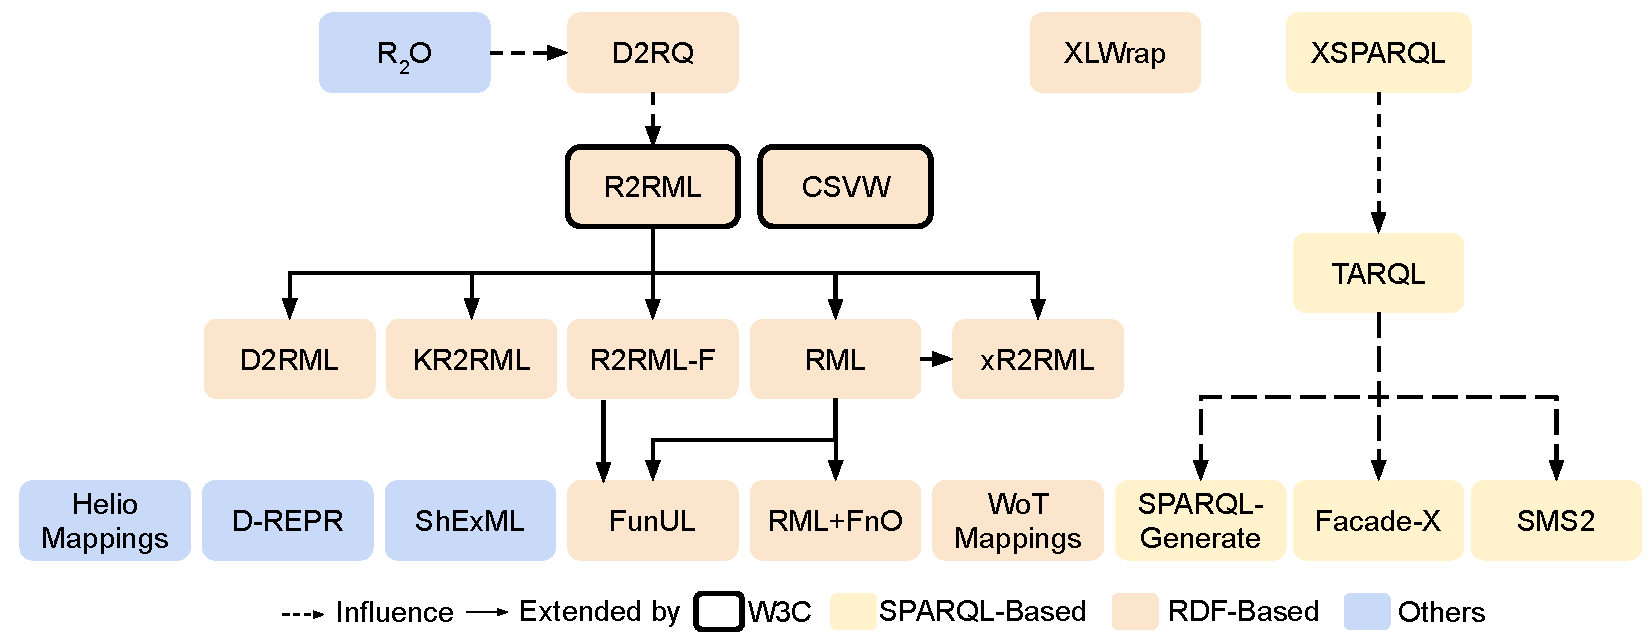
\includegraphics[width=0.95\linewidth]{figures/mapping_languages}
\caption{Existing mapping languages and their relationships.}
\label{fig:mapping_languages}
\end{figure*}

\noindent\paragraph{\textbf{RDF-based mapping languages.}} Similarly to Conceptual Mappings, these are mapping languages specified as ontologies. They are used as RDF documents that are processed by compliant tools for performing the translations. The evolution, extensions and influences on one another are depicted in \cref{fig:mapping_languages}. The most well-known language in this category is R2RML~\citep{das2012r2rml}, which allows mapping of data stored in relational databases to RDF. This language is heavily influenced by previous languages (R$_2$O~\citep{barrasa2004r2o} and D2RQ~\citep{bizer2004d2rq}). Some serializations (e.g. SML~\citep{Stadler2015sml}, OBDA mappings from Ontop~\citep{rodriguez2015efficient}) and several extensions of R2RML were developed in the following years after its release: R2RML-f~\citep{debruyne2016r2rmlf} extends R2RML to include functions to be applied over the data; RML~\citep{Dimou2014rml} and its user-friendly compact syntax YARRRML~\citep{Heyvaert2018yarrrml} provide the possibility of covering additional data formats (CSV, XML and JSON); this language also considers the use of functions for data transformation (e.g. lowercase, replace, trim) by using the Function Ontology (FnO)\footnote{\url{https://fno.io/rml/}}~\citep{DeMeester2017fno_dbpedia}; FunUL~\citep{junior2016funul} proposes an extension to also incorporate functions, but focusing on the CSV format; KR2RML~\citep{slepicka2015kr2rml} is also an extension for CSV, XML and JSON, with the addition of representing all sources with the Nested Relational Model as an intermediate model and the possibility of cleaning data with Python functions; xR2RML~\citep{michel2015xr2rml} extends R2RML and RML to include NoSQL databases and incorporates more features to handle tree-like data; D2RML~\citep{chortaras2018d2rml}, also based on R2RML and RML, is able to transform data from XML, JSON, CSVs and REST/SPARQL endpoints, and enables functions and conditions to create triples. 

In this category, we can also find more languages not related to R2RML. XLWrap~\citep{langegger2009xlwrap} is focused on transforming spreadsheets into different formats. CSVW~\citep{Tennison2015csvw} enables tabular data annotation on the Web with metadata, but also supports the generation of RDF. Finally, WoT Mappings~\citep{cimmino2020ewot} are oriented to be used in the context of the Web of Things.

\noindent\paragraph{\textbf{SPARQL-based mapping languages.}} The specification of this type of languages is usually based on, or is an extension of, the SPARQL query language~\citep{harris2013sparql}. XSPARQL~\citep{Bischof2012xsparql} merges SPARQL and XQuery to transform XML into RDF. TARQL~\citep{tarql} uses the SPARQL syntax to generate RDF from CSV files. SPARQL-Generate~\citep{Lefrancois2017sparqlgenerate} is capable of generating RDF and document streams from a wide variety of data formats and access protocols. Most recently, Facade-X has been developed, not as a new language, but as a "\textit{facade} to wrap the original resource and to make it queryable as if it was RDF"~\citep{asprino2023sparql-anything}. It does not extend the SPARQL language, instead it overrides the SERVICE operator. Lastly, authors would like to highlight a loosely SPARQL-based language, Stardog Mapping Syntax 2 (SMS2)~\citep{sms2}, which represents virtual Stardog graphs and is able to support sources such as JSON, CSV, RDB, MongoDB and Elasticsearch.

\noindent\paragraph{\textbf{Other mapping languages.}} This group gathers other mapping languages implemented without relying on ontologies or SPARQL extensions. ShExML~\citep{Garcia-Gonzalez2020shexml,garcia2021shexml-challenges} uses Shape Expressions (ShEx)~\citep{prud2014shex} to map data sources in RDBs, CSV, JSON, XML and RDF using SPARQL queries. The Helio mapping language~\citep{cimmino2022helio} is based on JSON and provides the capability of using functions for data transformation and data linking~\citep{cimmino2018hybrid}. D-REPR~\citep{Vu2019d-repr} focuses on describing heterogeneous data with JSONPath and allows the use of data transformation functions. XRM (Expressive RDF Mapper)~\citep{xrm} is a commercial language that provides a unique user-friendly syntax to create mappings in R2RML, CSVW and RML.


\subsection{Mapping serialisations}



\subsection{Mapping editors}



\subsection{Mapping language comparison}
As the number of mapping languages increased and their adoption grew wider, comparisons between these languages inevitably occurred. This is the case of, for instance, SPARQL-Generate~\citep{Lefrancois2017sparqlgenerate}, which is compared to RML in terms of query/mapping complexity; and ShExML~\citep{Garcia-Gonzalez2020shexml}, which is compared to SPARQL-Generate and YARRRML from a usability perspective.

Some studies dig deeper, providing qualitative complex comparison frameworks. Hert et al.~\citep{hert2011comparison} provide a comparison framework for mapping languages focused on transforming relational databases to RDF. The framework is composed of 15 features, and the languages are evaluated based on the presence or absence of these features.% (Logical table to class, M:N relationships, project attributes, select conditions, user-defined instance URIs, literal to URIs, vocabulary reuse, transformation functions, datatypes, named graphs, blank nodes, integrity constraints, static metadata, one table to \textit{n} classes, and write support). 
The results lead authors to divide the mappings into four categories (direct mapping, read-only general-purpose mapping, read-write general-purpose mapping, and special-purpose mapping), and ponder on the heavy reliance of most languages on SQL to implement the mapping, and the usefulness of read-write mappings (i.e., mappings able to write data in the database). De Meester et al.~\citep{DeMeester2019comparison} show an initial analysis of 5 similar languages (RML+FnO, xR2RML, FunUL, SPARQL-Generate, YARRRML) discussing their characteristics, according to three categories: non-functional, functional and data source support. The study concludes by remarking on the need to build a more complete and precise comparative framework and asking for a more active participation from the community to build it. To the best of our knowledge, there is no comprehensive work in the literature comparing all existing languages. \ana{ojo con esto que con el survey de ghent ya no es del todo cierto :(} 


\chapter{Objectives and Contributions}
\label{chapter:objectives}

This chapter presents the main objectives of this thesis and identifies the contributions to the state of the art. We enumerate the assumptions considered in this work, describe the main hypotheses and draw the limit of the scope of the thesis presenting the restrictions. \cref{fig:chp3_summary} provides an overview of the objectives and contributions presented in this thesis, along with their relations with identified hypotheses, assumptions and restrictions. 

\section{Objectives}
\label{sec:chp3-objectives}

%% PREVIOUS
% improve the mapping languages regarding expressiveness, usage and adoption to comply with the current evolving needs in knowledge graph construction

%% CURRENT LONG VERSION
%To advance the state of the art of declarative KGC technologies regarding support in language expressiveness, mapping writing and their role in KG evolution.

The general objective of this thesis is to \textit{improve the understanding (features and limitations) and operational management of declarative KG construction languages}. In order to achieve this goal, the following sub-objectives are defined:

\begin{enumerate}
    %\item[\textbf{O1.}] To analyse, understand and gather the capabilities of the mapping languages for KG construction from heterogeneous data sources.
    \item[\textbf{O1}]  To analyze the needs for declarative knowledge graph construction from heterogeneous data sources, in order to facilitate the support of advances in existing mapping languages to address the most relevant ones. 
    \item[\textbf{O2}] To help knowledge engineers and domain experts build declarative mappings in a user-friendly manner.
    \item[\textbf{O3}] To assess declarative knowledge graph construction technologies in terms of their benefits for supporting the creation and evolution of knowledge graphs. 
\end{enumerate}

In order to achieve the first objective, the following open research problem must be solved:
\begin{itemize}
    \item Ever since the first mapping languages began to be developed, many more have been proposed and released over the years. These languages address different needs and propose diverse features, but they share some characteristics, as in the end they all serve the same purpose of constructing KGs. In order to keep improving the KG construction process from heterogeneous sources, we need to identify which are the needs and the current challenges in the mapping languages. Thus we can facilitate the selection of languages according to their capabilities for addressing different needs. However, there is a lack of a fine-grained analysis of the competences and expressiveness of these mapping languages. %, as well as a formalization of their derived requirements. 
\end{itemize}

From a technological perspective, the following problem must be solved:
\begin{itemize}
    \item The needs for KG construction are not static, as they evolve with the use cases and evolution of surrounding technology. For instance, this is the case of the currently under development new specification of RDF 1.2~\parencite{hartig2023rdf}, that includes RDF-star triples. Mapping languages so far cannot produce RDF-star graphs without a dedicated extension, thus new technological support is needed to assist the creation of KGs with the evolving needs, and more specifically, to build RDF-star graphs. 
\end{itemize}

In order to achieve the second objective, the following research problem must be solved:
\begin{itemize}
    \item Most mapping languages are formalized as ontologies. In these cases, mappings are required to be written using an RDF serialization. Other common languages extend SPARQL to write transformation rules. This implies a double obstacle for new users, to learn the language and the language's syntax (i.e. Turtle or SPARQL) in case they are not familiar with them. There is a lack of methods that facilitate the writing process for both expert practitioners and new users to speed-up the process and become less error-prone.
    
    % while being up-to-date to the current needs in KG construction.
\end{itemize}

From a technological perspective, the following problem must be solved:
\begin{itemize}

    \item User-friendly approaches usually involve developing new syntaxes that cannot always be directly process by with KGC systems. In addition, different KGC systems are usually compliant with only one language. There is currently little interoperability among the existing languages, which limits the possibilities for users to use a wider variety of systems with different capabilities. Hence, new technological support is needed to allow translations among current mapping languages and reduce the barrier adoption enhancing the communication between user-friendly syntaxes and existing KGC implementations.   

\end{itemize}

Finally, for achieving the third objective, the following open research problem must be solved:

\begin{itemize}
    \item Knowledge graphs undergo a complex process from creation to consumption that comprise their life cycle. Declarative mapping rules and their supporting technologies are a key in the construction step, but can also play a beneficial role in other steps, such as data pre-processing and metadata annotation for transparency. However, there is a lack of research on their support in other tasks involved in the KG life cycle.
    %\textcolor{red}{Knowledge graphs are modeled according to schemes that are subject to changes over time. These modifications can be triggered by different factors, such as new requirements or error fixing, that can help improve the quality of the KG and the performance of downstream tasks that consume it. Graph re-construction can be achieved in different manners, but it is not known which approach perform best this task in different situations.} Thus, there is a lack of research on how mapping languages and compliant technology can assist this task to improve KG evolution. 
\end{itemize}

\section{Contributions}
\label{sec:chp3-contributions}

In this section, we describe the solutions corresponding to the objectives and open research problems described in \cref{sec:chp3-objectives}. We present as follows the contributions that support the advance of the current state of the art regarding the first objective (understand and gather the needs for KG construction): 

\begin{enumerate}
    \item[\textbf{C1}] Design of a \textbf{comparison framework analysing the state-of-the-art mapping languages} proposed to generate knowledge graphs from heterogeneous data sources. We extract the characteristics of these languages and compare them over a set of detailed features that show their expressiveness. 
    
    \item[\textbf{C2}] \textbf{Identification, definition and implementation of requirements for knowledge graph construction} from heterogeneous data sources. Based on the analysis performed on the comparison framework, we are able to extract what are the needs for building knowledge graphs, which are possible to achieve with the current languages and which need to be addressed yet. We implement these requirements in a formal language. 
    
    \item[\textbf{C3}] \textbf{Development of new features for the RML mapping language} to address the limitations of the language according to the new needs in knowledge graph construction. We focus on the development of the extension to create RDF-star graphs. 
\end{enumerate}

Regarding the second objective (to help knowledge engineers and domain experts to build mappings), we present new advances with the following contributions:

\begin{enumerate}
    \item[\textbf{C4}] \textbf{Design of a user-friendly approach for writing mapping rules based on spreadsheets}. We propose this approach as a way of writing mappings by only specifying the essential information, reducing learning curve of the language constructs and the syntax's peculiarities. We also develop an implementation of this approach to translate the mapping rules in spreadsheets into different mapping languages. 
    \item[\textbf{C5}] \textbf{Update of the YARRRML syntax for RML with new features}. We include in a new version of this syntax the features incorporated in the evolucion of the RML mapping language, to keep this language accessible for a broader community of users that already use YARRRML. We also provide an implementation to translate between the updated YARRRML version into other mapping languages to facilitate its adoption.
\end{enumerate}

Finally, with regard to the third objective (to assess the role of mapping technologies in KG evolution), this work presents the following contribution:

\begin{enumerate}
    \item[\textbf{C6}]\textbf{Analysis of the scenarios in which declarative KG construction technologies can play a valuable role in the evolution of knowledge graphs}. We conduct an evaluation to study how mapping-based processes be beneficial when the schema used in a knowledge graph changes with respect to other established methods.  %can not only be useful for KG construction, but also for facilitating the evolution of knowledge graphs that need a change in their schema. 
\end{enumerate}


\section{Assumptions}
\label{sec:chp3-assumptions}
Our work is based on the set of assumptions listed below. These assumptions provide a background to facilitate the comprehension of the decisions taken during the development of this work. 


\begin{enumerate}
    \item[\textbf{A1}] Mapping languages are declarative.
    \item[\textbf{A2}] Mapping languages provide human readable documentation available online.
    \item[\textbf{A3}] The schema of knowledge graphs (ontology) used for creating mapping documents is available and implemented in OWL or RDF(S). 
    \item[\textbf{A4}] Mapping rules can be translated into different languages with information preservation. 
    \item[\textbf{A5}] The evolution of the schema used in a KG does not involve changes in the data.
    %\item[\textbf{moar?}] KGs refer to RDF graphs?
\end{enumerate}


\section{Hypotheses}
\label{sec:chp3-hypotheses}

After the identification of the assumptions, we can describe the research hypotheses  of this thesis. They cover the general characteristics of the contributions:

\begin{enumerate}
    \item[\textbf{H1}] Current mapping languages lack some expressiveness to construct knowledge graphs from heterogeneous data sources for all use cases.
    \item[\textbf{H2}] It is possible to update  current mapping languages with new features that address the current needs in construction of knowledge graphs.
    \item[\textbf{H3}] Writing mapping rules in spreadsheet environments improves the user experience for practitioners of different backgrounds for writing mappings, whilst reducing errors. 
    \item[\textbf{H4}] Declarative KG construction technologies brings benefits in the evolution of knowledge graphs within their full life cycle.
\end{enumerate}


\section{Restrictions}
\label{sec:chp3-restrictions}

Finally, there is a set of restrictions that describe the limitations and define the future work objectives:

\begin{enumerate}
    \item[\textbf{R1}] Requirements for KG construction are considered up to January 2023, since it is an issue that is evolving during the time of writing this thesis.
    \item[\textbf{R2}] The reference for the RML specification in the mapping languages analysis is the release on 2014~\parencite{Dimou2014rml}.
    \item[\textbf{R3}] Features specific of non RDF-based mapping languages are not ensured to be modelled in an ontology (e.g. SPARQL recursive clauses, FILTER).
    \item[\textbf{R4}] The implementations proposed in contributions C4 and C5 are not fully compliant with all modules of the RML release on 2023~\parencite{iglesias2023rml}. 
    \item[\textbf{R5}] The evaluation of the value of mappings in KG evolution considers only schema changes, not data changes.
    \item[\textbf{R6}] The changes considered for KG evolution are schema changes for switching among metadata representation approaches for RDF graphs.
    %\item[\textbf{moar?}] algo de la selección de lenguajes? algo para mapeathor y yarrrml? The spreadsheet template consider the features of RML v2014 and the current RML-FNML spec. The YARRRML updates include all RMLv2 modules except for the RML-CC module.
\end{enumerate}


\begin{sidewaysfigure}[t!]
    \centering
    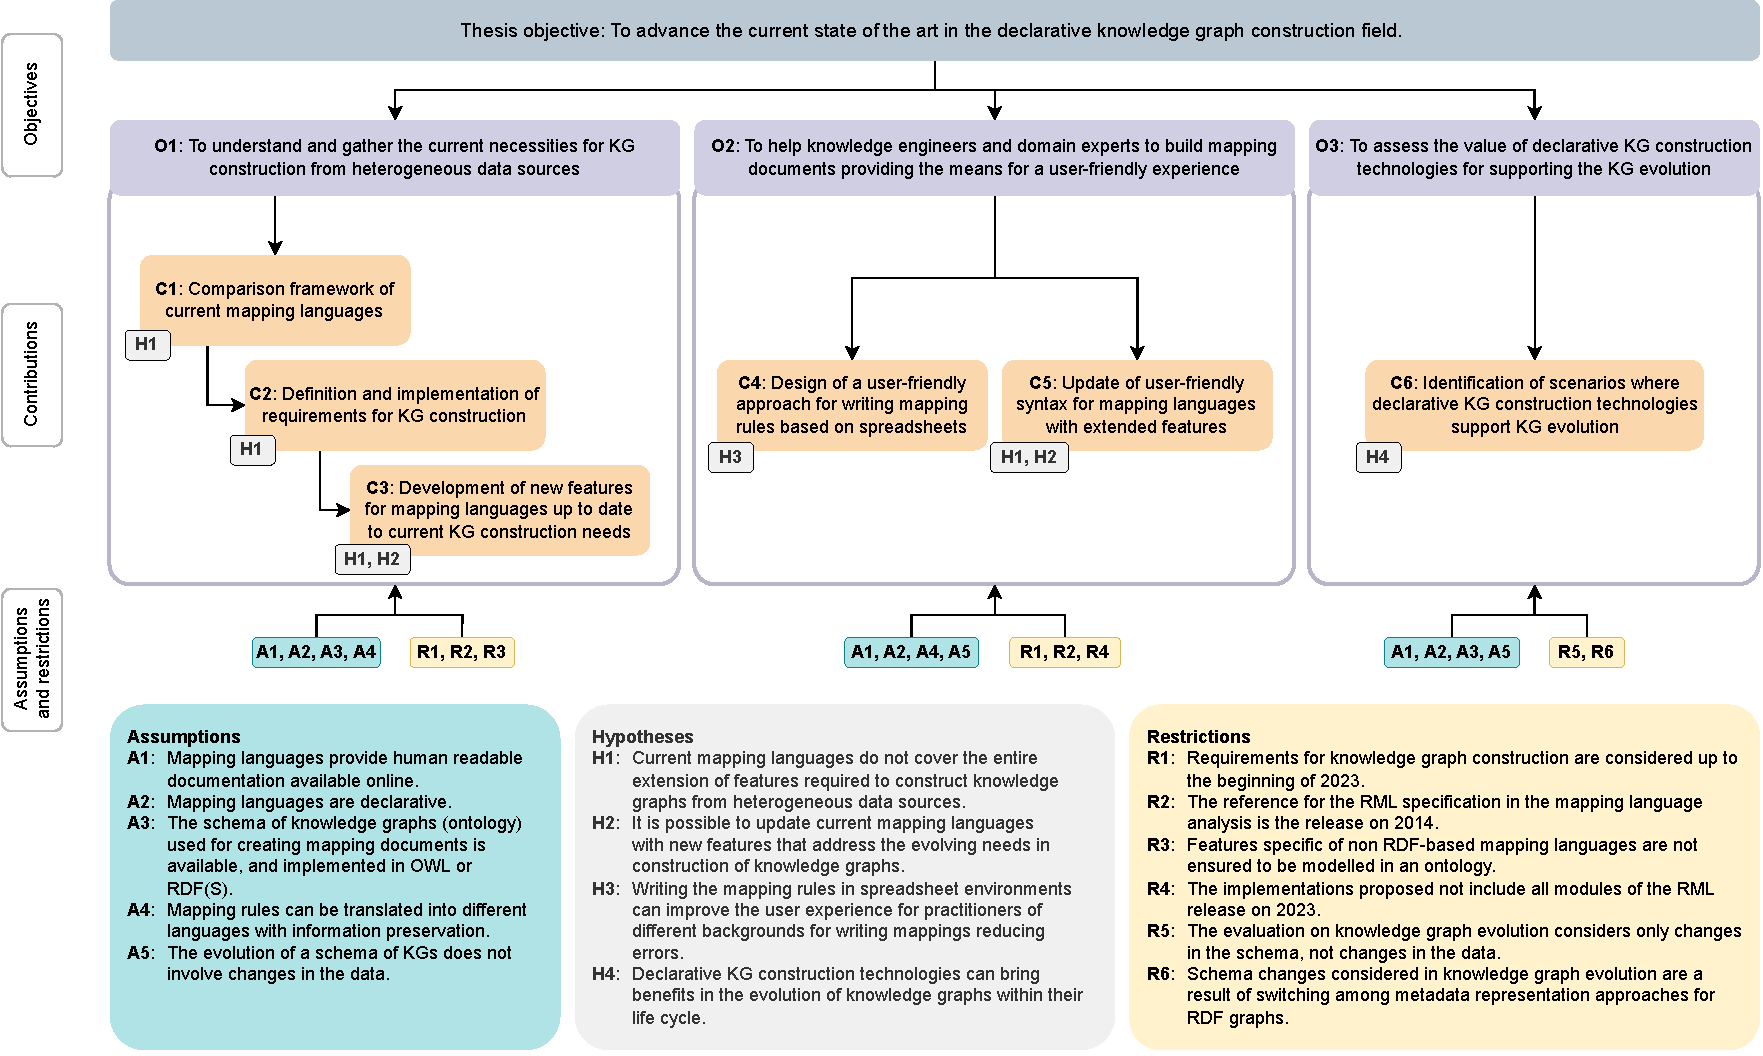
\includegraphics[width=1\linewidth]{figures/chp3_summary.pdf}
    \caption[Relations between objectives, contributions, hypotheses, assumptions and restrictions of this thesis]{Overview of objectives, contributions, hypotheses, assumptions and restrictions, and their relations.}
    \label{fig:chp3_summary}
\end{sidewaysfigure}

%\section{Research Methodology?}




\chapter{Mappings as the Key for Knowledge Graph Construction}
\label{chapter:mappings}

Mappings are the key element for the Knowledge Graph construction process to enhance maintainability, understandability and reproducibility. This chapter first presents an extensive analysis of current mapping languages in the form of a comparison framework. Based on this comparison, a set of requirements are extracted and used for building an ontology that aims at gathering the expressiveness of current mapping languages. Finally, the evolution of a well-known mapping language is presented for adopting RDF-star.

%\ana{al igual esta intro se puede extender más, explicando un poco más cada parte y situandola en su contexto, que no sea una enumeración de las subsecciones.}

\section{Comparison framework}
\label{sec:chp4_framework}


This section presents a comparison framework that collects and analyzes the main features included in mapping language descriptions. The diversity of the languages that have been analyzed is crucial for understanding the needs for constructing knowledge graphs from heterogeneous data sources. Thus, we can extract relevant shared features and requirements along with the peculiarities and innovations of each language. 

The framework presented in this section analyzes languages from the three categories identified in \cref{sec:chp2_mappings}. The selected languages fulfill the following requirements: (1) widely used, relevant and/or include novel or unique features; (2) currently maintained, and not deprecated; (3) not a serialization or a user-friendly representation of another language. For instance, D2RQ~\cite{bizer2004d2rq} and R$_2$O~\cite{barrasa2004r2o} were superseded by R2RML, which is included in the comparison. YARRRML~\cite{Heyvaert2018yarrrml} and XRM~\cite{xrm} are not included either, due to the fact that they provide a syntax for other already included languages (RML and R2RML; CSVW also for XRM).


The following RDF-based languages are included: R2RML~\cite{das2012r2rml}, RML~\cite{Dimou2014rml}, KR2RML~\cite{slepicka2015kr2rml}, xR2RML~\cite{michel2015xr2rml}, R2RML-F~\cite{debruyne2016r2rmlf}, FunUL~\cite{junior2016funul},  XLWrap~\cite{langegger2009xlwrap}, WoT mappings~\cite{cimmino2020ewot}, CSVW~\cite{Tennison2015csvw}, and D2\-RML~\cite{chortaras2018d2rml}. The analyzed SPARQL-based languages are: XSPARQL~\cite{Bischof2012xsparql}, TARQL~\cite{tarql},  SPARQL-Gene\-rate~\cite{Lefrancois2017sparqlgenerate}, SPARQL-Anything~\cite{asprino2023sparql-anything} and SMS2~\cite{sms2}. Finally, we selected the following languages based on other formats: ShExML~\cite{Garcia-Gonzalez2020shexml}, Helio Mappings~\cite{cimmino2022helio} and D-REPR~\cite{Vu2019d-repr}.  

These languages have been analyzed based on their official specification, documentation, or reference paper (listed in \cref{tab:chp2_languages_summary}). Specific implementations and extensions that are not included in the official documentation are not considered in this framework. The cells (i.e. language feature) marked "*"  in the framework tables indicate that there are non-official implementations or extensions that include the feature.

The framework has been built as a result of analyzing the common features of the aforementioned mapping languages, and also the specific features that make them unique and suitable for some scenarios. It includes information on data sources, general features for the construction of RDF graphs, and features related to the creation of subjects, predicates, and objects. In the following subsections, the features of each part of the framework are explained in detail. The language comparison for data sources is provided in \cref{tab:chp4_sources}, for triples creation in \cref{tab:chp4_spo}, and for general features in \cref{tab:chp4_metarules}. 

%Throughout the section, there are examples showing how different languages use the analyzed features. The example is built upon two input sources: an online JSON file, "coordinates.json", with geographical coordinates (\ref{fig:ex_json}); and a table from a MySQL database, "cities" (\ref{fig:ex_rdb}). The reference ontology is depicted in \ref{fig:ex_onto}. It represents information about cities and their locations. The expected RDF output of the data transformation is shown in \ref{lst:output}. Each mapping represents only the relevant rules that the subsection describes. The entire mapping can be found in the examples section of the ontology documentation\ref{foot:cmlink}. 




\subsection{Data Sources Description}


\cref{tab:chp4_sources} shows the ability of each mapping language to describe a data source in terms of retrieval, features, security, data format and protocol. 


\noindent\paragraph{\textbf{Data Retrieval.}} Data from data sources may be retrieved in a continuous manner (e.g., \textit{Streams}),  periodically (e.g., \textit{Asynchronous sources}), or just once, when the mapping is executed (e.g., \textit{Synchronous sources}). As shown in \cref{tab:chp4_sources}, all mapping languages are able to represent synchronous data sources. Additionally, SPARQL-Generate and Helio are able to represent periodical data sources, and SPARQL-Generate also represents continuous data sources (e.g. \texttt{it:WebSocket()} in SPARQL-Generate). Other languages do not explicitly express that feature in the language, but a compliant engine may implement it.

\noindent\paragraph{\textbf{Representing Data Sources.}} Extracting and retrieving heterogeneous data involves several elements that mapping languages need to consider: \textit{Security terms} to describe access (e.g., relational databases (RDB), API Key, OAuth2, etc); \textit{Retrieval protocol} such as local files, HTTP(S), JDBC, etc; \textit{Features that describe the data} to define particular characteristics of the source data (e.g. queries, regex, iterator, delimiter, etc); \textit{Data formats} such as CSV, RDB, and JSON; \textit{Encoding} and content negotiation (i.e. \textit{MIME Type}). 

Half of the languages do not allow the definition of security terms. Some languages are specific for RDB terms (R2RML and extensions, with \texttt{rr:logical\-Table}), and only two, Helio and WoT, can define security terms. These two languages are also the only ones that allow the specification of MIME Types, and can also specify the encoding along with TARQL and CSVW (e.g. \texttt{csvw:encoding} attribute of \texttt{csvw:Dialect} in CSVW). 

Regarding protocols, all languages consider local files, except WoT mappings, which are specific for HTTP(s). It is highly usual to consider HTTP(s) and database access (especially with the ODBC and JDBC protocols). Only XSPARQL, TARQL, D-REPR, and XLWrap describe exclusively local files. 

The features provided by each language are closely related to the data formats that are covered. Queries are usual for relational databases and NoSQL document stores and iterators for tree-like formats. Some languages also enable the description of delimiters and separators for tabular formats (e.g., CSVW defines the class \texttt{Dialect} to describe these features; this class is reused by RML), and finally, less common Regular Expressions can be defined to match specific parts of the data in languages such as CSVW, SPARQL-Generate, Helio, D-REPR, and D2RML (e.g., \texttt{RegexHandler} in Helio, \texttt{format} in CSVW). 

The most used format is tabular (RDB and CSV). Some languages can also process RDF graphs such as SMS2, ShExML, RML, SPARQL-Generate, Helio, and D2RML (e.g. \texttt{QUERY} in ShExML,  SPARQL service description\footnote{\url{http://www.w3.org/ns/sparql-service-description\#}} in RML), and the last three languages can also process plain text.


%\noindent\paragraph{\textbf{Data Sources Example.}} This example shows how ShExML and R2RML describe heterogeneous data sources. The sources are a table called "cities" (\ref{fig:ex_rdb}) that belongs to a relational database that stores information about cities: name, population, zipcode and year in which the data was updated; and a JSON file "coordinates.json" (\ref{fig:ex_json}) available online that contains the latitude and longitude of the central point of each city. R2RML is only able to describe the database table (\ref{lst:shexml_source}); instead ShExML is able to describe both the RDB and the online JSON file (\ref{lst:shexml_source}).


\begin{sidewaystable}[]
\centering
\caption[Comparison framework: Data source description]{Data retrieval and data source expression for the analysed mapping languages from the references stated in \cref{tab:chp2_languages_summary}. (*) indicates features not explicitly declared in the language, but that are implemented by compliant tools.}
\label{tab:chp4_sources}
\resizebox{1\textwidth}{!}{%
\def\arraystretch{2}
{\Huge
\begin{tabular}{l|l|c|c|c|c|c|c|c|c|c|c|c|c|c|c|c|c|c|c}
\multicolumn{2}{c|}{\textbf{Feature \textbackslash Language}} & \textbf{ShExML} & \textbf{XSPARQL} & \textbf{TARQL} & \textbf{CSVW} & \textbf{R2RML} & \textbf{RML} & \textbf{KR2RML} & \textbf{xR2RML} & \textbf{\begin{tabular}[c]{@{}c@{}}SPARQL-\\ Generate\end{tabular}} & \textbf{R2RML-F} & \textbf{FunUL} & \textbf{Helio} & \textbf{WoT} & \textbf{D-REPR} & \textbf{XLWrap} & \textbf{D2RML} & \textbf{\begin{tabular}[c]{@{}c@{}}SPARQL-\\ Anything\end{tabular}} & \textbf{SMS2} \\ \hline
\multirow{3}{*}{\begin{tabular}[c]{@{}l@{}}Retrieval \\ of data\end{tabular}} & Streams & false & false & false & false & false & true*\footnote{Implemented by RMLSreamer, available at \scriptsize\url{https://github.com/RMLio/RMLStreamer}.} & false & false & true & false & false & false & false & false & false & false & true & false\\ \cline{2-20} 
 & \begin{tabular}[c]{@{}l@{}}Synchronous \\ sources\end{tabular} & true & true & true & true & true & true & true & true & true & true & true & true & true & true & true & true & true & true \\ \cline{2-20} 
 & \begin{tabular}[c]{@{}l@{}}Asynchronous \\ sources\end{tabular} & - & - & - & - & - & - & - & - & Events, Periodic & - & - & Periodic & - & - & - & - & - & - \\ \hline
\multirow{6}{*}{\begin{tabular}[c]{@{}l@{}}Expressing \\ data sources\end{tabular}} & Security terms & - & - & - & - & \begin{tabular}[c]{@{}c@{}}Basic \\ (DB)\end{tabular} & \begin{tabular}[c]{@{}c@{}}Basic \\ (DB)\end{tabular} & \begin{tabular}[c]{@{}c@{}}Basic \\ (DB)\end{tabular} & \begin{tabular}[c]{@{}c@{}}Basic \\ (DB)\end{tabular} & - & \begin{tabular}[c]{@{}c@{}}Basic \\ (DB)\end{tabular} & - & \begin{tabular}[c]{@{}c@{}}API Key, OAuth2, \\ Bearer, Basic\end{tabular} & \begin{tabular}[c]{@{}c@{}}API Key, OAuth2, \\ Bearer, Basic\end{tabular} & - & - & \begin{tabular}[c]{@{}c@{}}Basic \\ (DB)\end{tabular} & - &  Basic (DB)\\ \cline{2-20} 
 & Encoding & false & false & true*\footnote{Command line input option \texttt{---encoding}~\cite{tarql}.} & true & false & true & false & false & false & false & false & true & true & false & false & false & true & \\ \cline{2-20} 
 & MIME Type & false & false & false & false & false & false & false & false & false & false & false & true & true & false & false & false & true & false \\ \cline{2-20} 
 & \begin{tabular}[c]{@{}l@{}}Features \\ describing data\end{tabular} & \begin{tabular}[c]{@{}l@{}}Iterator, \\ Queries\end{tabular} & - & \begin{tabular}[c]{@{}c@{}}Delimiter, \\ Separator\end{tabular} & \begin{tabular}[c]{@{}c@{}}Delimiter, \\ Separator, Regex\end{tabular} & Queries & \begin{tabular}[c]{@{}c@{}}Delimiter, Regex, \\ Iterator, Queries, \\ Separator\end{tabular} & Queries & \begin{tabular}[c]{@{}c@{}}Regex, \\ Iterator, Queries\end{tabular} & \begin{tabular}[c]{@{}c@{}}Delimiter, Regex, \\ Iterator, Queries, \\ Separator\end{tabular} & \begin{tabular}[c]{@{}c@{}}Iterator, \\ Queries\end{tabular} & \begin{tabular}[c]{@{}c@{}}Iterator, \\ Queries\end{tabular} & \begin{tabular}[c]{@{}c@{}}Delimiter, Regex, \\ Iterator, Queries, \\ Separator\end{tabular} & Iterator & \begin{tabular}[c]{@{}c@{}}Delimiter, \\ Regex, Iterator\end{tabular} & Separator & \begin{tabular}[c]{@{}c@{}}Delimiter, Regex, \\ Iterator, Queries\end{tabular} & \begin{tabular}[c]{@{}c@{}}Delimiter, Regex, \\ Iterator, Queries, \\ Separator\end{tabular} & \begin{tabular}[c]{@{}c@{}}Delimiter, Regex, \\ Iterator, Queries, \\ Separator\end{tabular} \\ \cline{2-20} 
 & \begin{tabular}[c]{@{}c@{}}Retrieval \\ protocol\end{tabular} & \begin{tabular}[c]{@{}c@{}}file, http(s), \\ odbc/jdbc\end{tabular} & file & file & file, http(s) & \begin{tabular}[c]{@{}c@{}}file, http(s), \\ odbc/jdbc\end{tabular} & \begin{tabular}[c]{@{}c@{}}file, http(s), \\ odbc/jdbc\end{tabular} & \begin{tabular}[c]{@{}c@{}}file, \\ odbc/jdbc\end{tabular} & \begin{tabular}[c]{@{}c@{}}file, \\ odbc/jdbc\end{tabular} & \begin{tabular}[c]{@{}c@{}}file, http(s), \\ odbc/jdbc \\ WebSocket, MQTT\end{tabular} & \begin{tabular}[c]{@{}c@{}}file, http(s), \\ odbc/jdbc\end{tabular} & file, http(s) & \begin{tabular}[c]{@{}c@{}}file, \\ any URI-based\end{tabular} & http(s) & file & file & \begin{tabular}[c]{@{}c@{}}file, http(s), \\ odbc/jdbc\end{tabular} & file, http(s) & file, odbc/jdbc\\ \cline{2-20} 
 & Data formats & \begin{tabular}[c]{@{}c@{}}Tabular, \\ Tree, Graph\end{tabular} & \begin{tabular}[c]{@{}c@{}}Tree \\ (XML)\end{tabular} & \begin{tabular}[c]{@{}c@{}}Tabular \\ (CSV)\end{tabular} & Tabular & Tabular & \begin{tabular}[c]{@{}c@{}}Tabular, \\ Tree, Graph\end{tabular} & \begin{tabular}[c]{@{}c@{}}Tabular, \\ Tree\end{tabular} & \begin{tabular}[c]{@{}c@{}}Tabular, \\ Tree\end{tabular} & \begin{tabular}[c]{@{}c@{}}Tabular, Tree, \\ Plain Text, Graph\end{tabular} & Tabular & \begin{tabular}[c]{@{}c@{}}Tabular, \\ Graph\end{tabular} & \begin{tabular}[c]{@{}c@{}}Tabular, Tree, \\ Plain Text, Graph\end{tabular} & Tree (JSON) & \begin{tabular}[c]{@{}c@{}}Tabular (CSV), \\ Tree\end{tabular} & \begin{tabular}[c]{@{}c@{}}Tabular \\ (CSV, Excel)\end{tabular} & \begin{tabular}[c]{@{}c@{}}Tabular, Tree, \\ Plain Text, Graph\end{tabular} & \begin{tabular}[c]{@{}c@{}}Tabular, Tree, \\ Plain Text, Graph\end{tabular} & \begin{tabular}[c]{@{}c@{}}Tabular, Tree, \\ Plain Text, Graph\end{tabular} \\
\end{tabular}%
}
}
\end{sidewaystable}





\subsection{Triples Generation}
\cref{tab:chp4_spo} represents how different languages describe the generation of triples. We assess whether they generate the \textit{Subject}, \textit{Predicate}, and \textit{Object}: in (1) a \textit{Constant} manner, i.e. non-dependant on the data field to be created; or in (2) a \textit{Dynamic} manner, i.e. changing its value with each data field iteration. For \textit{Objects}, the possibility of adding \textit{Datatype and Language} tags is also considered; this feature assesses whether they can be added, and if they are added in a dynamic (changes with the data) or static (constant) manner. This table also analyzes the use and cardinality of transformation functions and the possibility of iterating over different nested level arrays (i.e., in tree-like formats).

The categories \textit{Constant} and \textit{RDF Resource} (the latter within \textit{Dynamic}) show which kind of resources can be generated by the language (i.e., IRI, Blank Node, Literal, List and/or Container). The \textit{Dynamic} category also considers: the \textit{Data References} (i.e. fields from the data source) that can appear with single of mixed formats; from how many \textit{Data Sources} (e.g. ```1:1" when only data from one file can be used) the term is generated; if \textit{Hierarchy Iteration} over different nested levels in tree-like formats is allowed; and if \textit{Functions} can be used to perform transformations on the data to create the term (e.g. \texttt{lowercase}, \texttt{toDate}, etc.).

\noindent\paragraph{\textbf{Subject Generation.}} Subjects can be IRIs or Blank Nodes (BN). This is well reflected in the languages, since, with a few exceptions that do not consider Blank Nodes, all languages are able to generate these two types of RDF resources, both constant and dynamically. The WoT mappings can only generate constant subjects, so the dynamic dimensions do not apply to this language. The rest of the languages can generate a subject with one or more data references (e.g., in RML \texttt{rr:template "http://ex.org/\{id\}\-\{name\}"}), ShExML, xR2R\-ML, SPARQL-Generate, Facade-X, and Helio with different formats. For example, in xR2RML a CSV field that contains an array can be expressed as: \texttt{xrr:reference "Column(Mo\-vies)/JSONPath(\$.*)}. Part of the languages even allow generating subjects with more than one data source, this is the case of ShExML, XSPARQL, KR2RML, SPARQL-Generate, Facade-X, Helio and xR2RML. About a third of the languages allow hierarchy iterations (ShExML, XSPARQL, KR2RML, SPARQL-Generate, D-REPR, Facade-X, SMS2, and D2RML), and more than a half use functions with N:1 cardinality. Additionally, some of them even allow functions that can output more than one parameter (i.e., 1:N or N:M), but it is less usual.



\noindent\paragraph{\textbf{Predicate Generation.}} All languages can generate constant predicates as IRIs. Only four languages do not allow dynamic predicates (WoT mappings, SMS2, ShExML, and XLWrap). For those that do, they also allow more than one data reference. The languages that allow subject generation using multiple formats, data sources, functions, and hierarchy iterations, provide the same features for predicate generation.

\noindent\paragraph{\textbf{Object Generation.}} %There is a wider variety of RDF resources that the considered languages can generate,
Generally, languages can generate a wider range of resources for objects, since they can be IRIs, blank nodes, literals, lists, or containers. All of them can generate constant and dynamic literals and IRIs. Those languages that allow blank nodes in the subject also allow them in the object. Additionally, ShExML, KR2RML, SPARQL-Generate, Facade-X, xR2RML, and WoT mappings consider lists, and the last two languages also consider containers (e.g. \texttt{rr:termType xrr:RdfBag} in xR2RML). Data references, sources, hierarchy iterations, and functions remain the same as in subject generation, with the addition of WoT mappings that allow dynamic objects. Lastly, datatype and language tags are not allowed in KR2RML and XLWrap; they are defined as constants in the rest of the languages, and dynamically in ShExML, XSPARQL, TARQL, RML, and Helio (e.g., \texttt{rml:languageMap} for dynamic language tags in RML).

%

\begin{sidewaystable}[]
\centering
\caption[Comparison framework: Triple generation]{Features for subject, predicate, and object generation of the studied mapping languages from the references stated in \cref{tab:chp2_languages_summary}.}
\label{tab:chp4_spo}
\resizebox{\textwidth}{!}{%
\def\arraystretch{2}
\begin{tabular}{l|l|l|c|c|c|c|c|c|c|c|c|c|c|c|c|c|c|c|c|c}
\multicolumn{3}{c|}{\textbf{Feature \& Language}} & \textbf{ShExML} & \textbf{XSPARQL} & \textbf{TARQL} & \textbf{CSVW} & \textbf{R2RML} & \textbf{RML} & \textbf{KR2RML} & \textbf{xR2RML} & \textbf{\begin{tabular}[c]{@{}c@{}}SPARQL-\\Generate\end{tabular}} & \textbf{R2RML-F} & \textbf{FunUL} & \textbf{Helio} & \textbf{WoT} & \textbf{D-REPR} &\textbf{ XLWrap} & \textbf{D2RML} & \textbf{\begin{tabular}[c]{@{}c@{}}SPARQL-\\ Anything\end{tabular}} & \textbf{SMS2} \\ \hline
\multicolumn{1}{c|}{\multirow{6}{*}{Subject}} & \multicolumn{2}{l|}{Constant} & IRI & BN, IRI & BN, IRI & IRI & BN, IRI & BN, IRI & - & BN, IRI & BN, IRI & BN, IRI & BN, IRI & IRI & IRI & BN, IRI & BN, IRI & BN, IRI & BN, IRI & BN, IRI \\ \cline{2-21} 
\multicolumn{1}{c|}{} & \multirow{5}{*}{Dynamic} & RDF Resource & IRI & BN, IRI & BN, IRI & IRI & BN, IRI & BN, IRI & IRI & BN, IRI & IRI & BN, IRI & BN, IRI & IRI & - & BN, IRI & BN, IRI & BN, IRI & IRI & BN, IRI\\ \cline{3-21} 
\multicolumn{1}{c|}{} &  & Data Reference & \begin{tabular}[c]{@{}c@{}}1..* Ref\\ 1..* Format\end{tabular} & \begin{tabular}[c]{@{}c@{}}1..* Ref\\ 1..1 Format\end{tabular} & \begin{tabular}[c]{@{}c@{}}1..* Ref\\ 1..1 Format\end{tabular} & \begin{tabular}[c]{@{}c@{}}1..* Ref\\ 1..1 Format\end{tabular} & \begin{tabular}[c]{@{}c@{}}1..* Ref\\ 1..1 Format\end{tabular} & \begin{tabular}[c]{@{}c@{}}1..* Ref\\ 1..1 Format\end{tabular} & \begin{tabular}[c]{@{}c@{}}1..* Ref\\ 1..* Format\end{tabular} & \begin{tabular}[c]{@{}c@{}}1..* Ref\\ 1..* Format\end{tabular} & \begin{tabular}[c]{@{}c@{}}1..* Ref\\ 1..1 Format\end{tabular} & \begin{tabular}[c]{@{}c@{}}1..* Ref\\ 1..1 Format\end{tabular} & \begin{tabular}[c]{@{}c@{}}1..* Ref\\ 1..1 Format\end{tabular} & \begin{tabular}[c]{@{}c@{}}1..* Ref\\ 1..* Format\end{tabular} & \begin{tabular}[c]{@{}c@{}}-\end{tabular} & \begin{tabular}[c]{@{}c@{}}1..* Ref\\ 1..1 Format\end{tabular} & \begin{tabular}[c]{@{}c@{}}1..* Ref\\ 1..1 Format\end{tabular} & \begin{tabular}[c]{@{}c@{}}1..* Ref\\ 1..1 Format\end{tabular} &
\begin{tabular}[c]{@{}c@{}}1..* Ref\\ 1..* Format\end{tabular}& \begin{tabular}[c]{@{}c@{}}1..* Ref\\ 1..1 Format\end{tabular}  \\ \cline{3-21} 
\multicolumn{1}{c|}{} &  & Data Sources & 1..* & 1..* & 1..1 & 1..1 & 1..1 & 1..1 & 1..* & 1..* & 1..* & 1..1 & 1..1 & 1..* & - & 1..1 & 1..1 & 1..1  & 1..* & 1..1 \\ \cline{3-21} 
\multicolumn{1}{c|}{} &  & Hierarchy Iteration & true & true & false & false & false & true & true & false & true & false & false & false & false & true & false & true & true & true\\ \cline{3-21} 
\multicolumn{1}{c|}{} &  & Functions & - & 1..* & 1..* & - & - & 1..* & 1..* & - & 1..* & 1..* & 1..* & 1..* & - & 1..* & 1..* & 1..* & 1..* & 1..* \\ \hline
\multirow{6}{*}{Predicate} & \multicolumn{2}{l|}{Constant} & IRI & IRI & IRI & IRI & IRI & IRI & IRI & IRI & IRI & IRI & IRI & IRI & IRI & IRI & IRI & IRI & IRI &\\ \cline{2-21} 
 & \multirow{5}{*}{Dynamic} & RDF Resource & - & IRI & IRI & IRI & IRI & IRI & IRI & IRI & IRI & IRI & IRI & IRI & - & IRI & - & IRI & IRI & IRI\\ \cline{3-21} 
 &  & Data Reference & - & \begin{tabular}[c]{@{}c@{}}1..* Ref\\ 1..1 Format\end{tabular} & \begin{tabular}[c]{@{}c@{}}1..* Ref\\ 1..1 Format\end{tabular} & \begin{tabular}[c]{@{}c@{}}1..* Ref\\ 1..1 Format\end{tabular} & \begin{tabular}[c]{@{}c@{}}1..* Ref\\ 1..1 Format\end{tabular} & \begin{tabular}[c]{@{}c@{}}1..* Ref\\ 1..1 Format\end{tabular} & \begin{tabular}[c]{@{}c@{}}1..* Ref\\ 1..* Format\end{tabular} & \begin{tabular}[c]{@{}c@{}}1..* Ref\\ 1..1 Format\end{tabular} & \begin{tabular}[c]{@{}c@{}}1..* Ref\\ 1..1 Format\end{tabular} & \begin{tabular}[c]{@{}c@{}}1..* Ref\\ 1..1 Format\end{tabular} & \begin{tabular}[c]{@{}c@{}}1..* Ref\\ 1..1 Format\end{tabular} & \begin{tabular}[c]{@{}c@{}}1..* Ref\\ 1..* Format\end{tabular} & \begin{tabular}[c]{@{}c@{}}-\end{tabular} & \begin{tabular}[c]{@{}c@{}}1..* Ref\\ 1..1 Format\end{tabular} & \begin{tabular}[c]{@{}c@{}}-\end{tabular} & \begin{tabular}[c]{@{}c@{}}1..* Ref\\ 1..1 Format\end{tabular} & \begin{tabular}[c]{@{}c@{}}1..* Ref\\ 1..* Format\end{tabular}
 & -\\ \cline{3-21} 
 &  & Data Sources & - & 1..1 & 1..1 & 1..1 & 1..1 & 1..1 & 1..* & 1..1 & 1..* & 1..1 & 1..1 & 1..* & - & 1..1 & - & 1..1 & 1..* & - \\ \cline{3-21} 
 &  & Hierarchy Iteration & false & false & false & false & false & true & true & false & false & false & false & false & false & true & false & true & true & false \\ \cline{3-21} 
 &  & Functions & - & 1..* & 1..* & - & - & 1..* & 1..* & - & 1..* & 1..* & 1..* & 1..* & - & 1..* & - & 1..* & 1..* & -\\ \hline
\multirow{7}{*}{Object} & \multicolumn{2}{l|}{Constant} & IRI, Literal & \begin{tabular}[c]{@{}c@{}}BN, IRI, \\ Literal\end{tabular} & \begin{tabular}[c]{@{}c@{}}BN, IRI, \\ Literal\end{tabular} & IRI, Literal & IRI, Literal & IRI, Literal & IRI, Literal & \begin{tabular}[c]{@{}c@{}}BN, IRI, Literal,\\ List, Container\end{tabular} & \begin{tabular}[c]{@{}c@{}}BN, IRI, \\ Literal, List\end{tabular} & IRI, Literal & IRI, Literal & IRI, Literal & \begin{tabular}[c]{@{}c@{}}BN, IRI, Literal, \\ List, Container\end{tabular} & \begin{tabular}[c]{@{}c@{}}BN, IRI, \\ Literal\end{tabular} & IRI, Literal & \begin{tabular}[c]{@{}c@{}}BN, IRI, \\ Literal\end{tabular} & \begin{tabular}[c]{@{}c@{}}BN, IRI, \\ Literal, List\end{tabular} & \begin{tabular}[c]{@{}c@{}}BN, IRI, \\ Literal\end{tabular} \\ \cline{2-21} 
 & \multirow{5}{*}{Dynamic} & RDF Resource & \begin{tabular}[c]{@{}c@{}}IRI, Literal,\\ Lists\end{tabular} & \begin{tabular}[c]{@{}c@{}}BN, IRI, \\ Literal\end{tabular} & \begin{tabular}[c]{@{}c@{}}BN, IRI, \\ Literal\end{tabular} & IRI, Literal & \begin{tabular}[c]{@{}c@{}}BN, IRI, \\ Literal\end{tabular} & \begin{tabular}[c]{@{}c@{}}BN, IRI, \\ Literal\end{tabular} & \begin{tabular}[c]{@{}c@{}}IRI, Literal,\\ List\end{tabular} & \begin{tabular}[c]{@{}c@{}}BN, IRI, Literal,\\ List, Container\end{tabular} & \begin{tabular}[c]{@{}c@{}}BN, IRI, \\ Literal, List\end{tabular} & \begin{tabular}[c]{@{}c@{}}BN, IRI, \\ Literal\end{tabular} & \begin{tabular}[c]{@{}c@{}}BN, IRI, \\ Literal\end{tabular} & IRI, Literal & IRI, Literal & \begin{tabular}[c]{@{}c@{}}BN, IRI, \\ Literal\end{tabular} & IRI, Literal & \begin{tabular}[c]{@{}c@{}}BN, IRI, \\ Literal\end{tabular} & \begin{tabular}[c]{@{}c@{}}BN, IRI, \\ Literal, List\end{tabular} & \begin{tabular}[c]{@{}c@{}}BN, IRI, \\ Literal\end{tabular}\\ \cline{3-21} 
 &  & Data Reference & \begin{tabular}[c]{@{}c@{}}1..* Ref\\ 1..* Format\end{tabular} & \begin{tabular}[c]{@{}c@{}}1..* Ref\\ 1..1 Format\end{tabular} & \begin{tabular}[c]{@{}c@{}}1..* Ref\\ 1..1 Format\end{tabular} & \begin{tabular}[c]{@{}c@{}}1..* Ref\\ 1..1 Format\end{tabular} & \begin{tabular}[c]{@{}c@{}}1..* Ref\\ 1..1 Format\end{tabular} & \begin{tabular}[c]{@{}c@{}}1..* Ref\\ 1..1 Format\end{tabular} & \begin{tabular}[c]{@{}c@{}}1..* Ref\\ 1..* Format\end{tabular} & \begin{tabular}[c]{@{}c@{}}1..* Ref\\ 1..* Format\end{tabular} & \begin{tabular}[c]{@{}c@{}}1..* Ref\\ 1..1 Format\end{tabular} & \begin{tabular}[c]{@{}c@{}}1..* Ref\\ 1..1 Format\end{tabular} & \begin{tabular}[c]{@{}c@{}}1..* Ref\\ 1..1 Format\end{tabular} & \begin{tabular}[c]{@{}c@{}}1..* Ref\\ 1..* Format\end{tabular} & \begin{tabular}[c]{@{}c@{}}-\end{tabular} & \begin{tabular}[c]{@{}c@{}}1..* Ref\\ 1..1 Format\end{tabular} & \begin{tabular}[c]{@{}c@{}}1..* Ref\\ 1..1 Format\end{tabular} & \begin{tabular}[c]{@{}c@{}}1..* Ref\\ 1..1 Format\end{tabular} & \begin{tabular}[c]{@{}c@{}}1..* Ref\\ 1..* Format\end{tabular} &
 \begin{tabular}[c]{@{}c@{}}1..* Ref\\ 1..1 Format\end{tabular}\\ \cline{3-21} 
 &  & Data Sources & 1..* & 1..* & 1..1 & 1..1 & 1..1 & 1..1 & 1..* & 1..* & 1..* & 1..1 & 1..1 & 1..* & - & 1..1 & 1..1 & 1..1 & 1..* & 1..1 \\ \cline{3-21} 
 &  & Hierarchy Iteration & true & true & false & false & false & true & true & false & true & false & false & false & false & true & false & true & true & true \\ \cline{3-21} 
 &  & Functions & 1 & 1..* & 1..* & - & - & 1..* & 1..* & - & 1..* & 1..* & 1..* & 1..* & - & 1..* & 1..* & 1..* & 1..* & 1..* \\ \cline{2-21} 
 & \multicolumn{2}{l|}{Datatype and Language} & \begin{tabular}[c]{@{}c@{}}static,\\ dynamic\end{tabular} & \begin{tabular}[c]{@{}c@{}}static,\\ dynamic\end{tabular} & \begin{tabular}[c]{@{}c@{}}static,\\ dynamic\end{tabular} & static & static & \begin{tabular}[c]{@{}c@{}}static,\\ dynamic\end{tabular} & - & static & static & static & static & \begin{tabular}[c]{@{}c@{}}static,\\ dynamic\end{tabular} & static & static & - & static & static & static \\ 
\end{tabular}%
}
\end{sidewaystable}








\subsection{General Features for Graph Construction}

\cref{tab:chp4_metarules} shows the features of mapping languages regarding the %generation of triples  
construction of RDF graphs such as \textit{linking rules}, \textit{metadata} or \textit{conditions}, assignment to \textit{named graphs}, and declaration of \textit{transformation functions} within the mapping. 

\noindent\paragraph{\textbf{Statements.}} General features that apply to statements are described in this section: the capability of a language to assign statements to \textit{named graphs}, to \textit{retrieve data from only one source} or \textit{more than one source}, and to apply \textit{conditions} that have to be met in order to create the statement (e.g. if the value of a field called "required" is \texttt{TRUE}, the triple is generated).

Most RDF-based languages allow static assignment to named graphs. R2RML, RML, R2RML-F, FunUL, and D2RML enable also dynamic definitions (e.g., \texttt{rr:graph\-Map} in R2RML and in its extensions). Theoretically, the rest of R2RML extensions should also implement this feature; however, to the best of our knowledge, it is not mentioned in their respective specifications. 

Allowing conditional statements is not usual; it is only considered in the SPARQL-based languages (with the exception of SMS2), XLWrap and D2RML (e.g. \texttt{xl:breakCo\-ndition} in XLWrap). Regarding data sources, all languages allow data retrieval from at least one source; ShExML, XSPARQL, CSVW, SPARQL-Generate, Facade-X, Helio, D-REPR and D2RML enable more sources. That is, using data in the same statement from, e.g., one CSV file and one JSON file.


\noindent\paragraph{\textbf{Linking Rules.}} Linking rules refer to linking resources that are being created in the mapping. For instance, having as object of a statement a resource that is the subject of another statement. These links are implemented in most languages by joining one or more data fields. Six languages do not allow these links: TARQL, CSVW, KR2RML, WoT, SMS2, and XLWrap. The rest is able to perform linking with at least one data reference and one or no condition. Fewer enable more data references and more conditions (e.g. in R2RML and most extensions allow the application of a \texttt{rr:joinCondition} over several fields). 

Linking rules using join conditions imply evaluating if the fields selected are equal. Since the join condition is the most common, applying the equal logical operator is the preferred choice. Only a few languages consider other similarity functions to perform link discovery, such as the Levenshtein distance and Jaro-Winkler, e.g., Helio. %Finally, it may be highlighted the ability for some languages to perform other logical operators appart from join, such as union (e.g. ShExML, KR2RML).




\noindent\paragraph{\textbf{Transformation functions.}} Applying functions in mappings allows practitioners transforming data before it is translated. For instance, to generate a label with an initial capital letter (\texttt{ex:ID001 rdfs:label "Emily"}) that was originally in lower case (```emily"), a function may be applied (e.g. GREL function \texttt{toTi\-tleCase()}). Only four of the analyzed languages do not allow the use of these functions: CSVW, R2RML, xR2RML, and  WoT mappings. Of those that do, some use functions that belong to a specification (e.g. RML+FnO uses GREL functions\footnote{\url{https://docs.openrefine.org/manual/grelfunctions}}). All of them consider functions with cardinalities 1:1 and N:1; and half of them also include 1:N and N:M (i.e., output more than one value), for instance, a regular expression that matches and returns more than one value.  Nesting functions (i.e. calling a function inside another function) is not unusual; this is the case of SPARQL-based languages, the R2RML extensions that implement functions (except K2RML), Helio, D-REPR, and XLWrap. Finally, some languages even enable extending functions depending on specific user needs, such as XSPARQL, RML+FnO, SPARQL-Generate, Facade-X, R2RML-F, FunUL, XLWrap and D2RML.

%\noindent\paragraph{\textbf{Graph Construction Example.}} Assuming the description of data sources shown in \ref{fig:ex_json} and \ref{fig:ex_rdb} and the regular triples, this example shows how Helio and SPARQL-Generate describe conditional statements and linking rules. To generate the \texttt{eg:pop\-ulation} attribute (\ref{fig:ex_onto}), the record must have been updated after 2020. In addition, instances of the classes \texttt{eg:City} and \texttt{eg:Location} can be joined using the city name, present in both data sources. However, the names do not exactly match ("Almería" and "Almeria"; "A Coruña" and "La Coru\-ña"), which is why a distance metric is required to match the cities with a threshold of 0.75. The Helio mapping is not capable of describing the condition of the population, but instead it is able to use the Levenshtein distance function and link the sources (\ref{lst:helio_general}). SPARQL-Generate can describe the condition statement thanks to the SPARQL construct \texttt{FILTER}, but does not implement the distance metric function (\ref{lst:sg_general}). However, both Helio and SPARQL-Generate allow the removal of spaces in the subject URIs. 

\begin{sidewaystable}[]
\centering
%\rotatebox{180}{
\begin{minipage}{21.5cm}
\caption[Comparison Framework: General features]{Statements, linking rules, and function properties of the studied mapping languages from the references stated in \cref{tab:chp2_languages_summary}.}
\label{tab:chp4_metarules}
\resizebox{\textwidth}{!}{%
\def\arraystretch{1.5}
\begin{tabular}{c|l|c|c|c|c|c|c|c|c|c|c|c|c|c|c|c|c|c|c}
\multicolumn{2}{c|}{\textbf{Feature \textbackslash Language}} & \textbf{ShExML} & \textbf{XSPARQL} & \textbf{TARQL} & \textbf{CSVW} & \textbf{R2RML} & \textbf{RML} & \textbf{KR2RML} & \textbf{xR2RML} & \textbf{\begin{tabular}[c]{@{}c@{}}SPARQL-\\Generate\end{tabular}} & \textbf{R2RML-F} & \textbf{FunUL} & \textbf{Helio} & \textbf{WoT} & \textbf{D-REPR} & \textbf{XLWrap} & \textbf{D2RML} & \textbf{\begin{tabular}[c]{@{}c@{}}SPARQL-\\Anything\end{tabular}} & \textbf{SMS2} \\ \hline
\multirow{5}{*}{Statements} & Assign to named graphs & static & - & - & - & \begin{tabular}[c]{@{}c@{}}static, \\ dynamic\end{tabular} & \begin{tabular}[c]{@{}c@{}}static, \\ dynamic\end{tabular} & static & static & - & \begin{tabular}[c]{@{}c@{}}static, \\ dynamic\end{tabular} & \begin{tabular}[c]{@{}c@{}}static, \\ dynamic\end{tabular} & - & - & - & static & \begin{tabular}[c]{@{}c@{}}static, \\ dynamic\end{tabular} & - & - \\ \cline{2-20} 
 & \begin{tabular}[c]{@{}l@{}}Retrieve data from \\  one source\end{tabular} & true & true & true & true & true & true & true & true & true & true & true & true & true & true & true & true & true & true \\ \cline{2-20} 
 & \begin{tabular}[c]{@{}l@{}}Retrieve data from \\ one or more sources\end{tabular} & true & true & false & true & false & false & false & false & true & false & false & true & false & true & false & true & true & false \\ \cline{2-20} 
 & \begin{tabular}[c]{@{}l@{}}Allow conditions \\ to form statements\end{tabular} & true & true & true & false & false & false & false & false & true & false & false & false & false & false & true & true & true & false \\ \hline
\multirow{7}{*}{Linking rules} & Use one data reference & true & true & false & true & true & true & false & true & true & true & true & true & true & true & false & true & true & false \\ \cline{2-20} 
 & \begin{tabular}[c]{@{}l@{}}Use one or more \\ data reference\end{tabular} & true & false & false & false & false & true & false & true & true & false & false & true & false & true & false & false & true & false \\ \cline{2-20} 
 & No condition to link & true & true & false & false & true & true & false & true & true & true & true & true & false & false & false & true & true & false \\ \cline{2-20} 
 & Link with one condition & true & true & false & false & true & true & false & true & true & true & true & true & false & true & false & true & true & false \\ \cline{2-20} 
 & \begin{tabular}[c]{@{}l@{}}Link with one or \\ more conditions\end{tabular} & false & true & false & false & true & true & false & true & true & true & true & true & false & true & false & true & true & false \\ \cline{2-20} 
 & \begin{tabular}[c]{@{}l@{}}Use only equal \\ function in condition\end{tabular} & true & true & false & false & true & true & false & true & true & true & true & true & false & true & false & true & true & false \\ \cline{2-20} 
 & \begin{tabular}[c]{@{}l@{}}Use any similarity \\ function in condition\end{tabular} & false & true & false & false & false & true & false & false & false & false & false & true & false & false & false & true & true & false \\ \hline
\multirow{5}{*}{Functions} & Cardinality & 1:1, N:1 & \begin{tabular}[c]{@{}c@{}}1:1, N:1, \\ 1:N, N:M\end{tabular} & 1:1, N:1 & - & - & 1:1, N:1*\footnote{With the Function Ontology (FnO)~\cite{DeMeester2017fno_dbpedia}}  & \begin{tabular}[c]{@{}c@{}}1:1, N:1, \\ 1:N, N:M\end{tabular} & - & \begin{tabular}[c]{@{}c@{}}1:1, N:1, \\ 1:N, N:M\end{tabular} & 1:1, N:1 & 1:1, N:1 & 1:1, N:1 & - & \begin{tabular}[c]{@{}c@{}}1:1, N:1, \\ 1:N, N:M\end{tabular} & \begin{tabular}[c]{@{}c@{}}1:1, N:1, \\ 1:N, N:M\end{tabular} & \begin{tabular}[c]{@{}c@{}}1:1, N:1, \\ 1:N, N:M\end{tabular} & \begin{tabular}[c]{@{}c@{}}1:1, N:1, \\ 1:N, N:M\end{tabular} & 
\begin{tabular}[c]{@{}c@{}}1:1, N:1, \\ 1:N, N:M\end{tabular} \\ \cline{2-20} 
 & Nested functions & false & true & true & false & false & true*$^{a}$ & false & false & true & true & true & true & false & true & true & true & true & true \\ \cline{2-20} 
 & \begin{tabular}[c]{@{}l@{}}Functions belong \\ to a specification\end{tabular} & true & false & true & false & false & true*$^{a}$ & false & false & true & false & false & true & false & false & true & false & true & true \\ \cline{2-20} 
 & \begin{tabular}[c]{@{}l@{}}Declare own \\ functions\end{tabular} & true & true & false & false & false & true*$^{a}$ & false & false & true & true & true & false & false & false & true & true & true & false \\ %\cline{2-18} 
 %& \begin{tabular}[c]{@{}l@{}}Implementation \\ ready to use\end{tabular} & false & - & true & false & false & true & true & false & true & false & false & true & false & false & true & false \\ 
\end{tabular} 
}
\end{minipage}%}
\end{sidewaystable}


\section{Mapping Rules for RDF: Conceptual Mapping}
\label{sec:chp4_cm_ontology}

Based on the analysis performed in \cref{sec:chp4_framework}, we abstract the features and limitations present in current mapping languages to represent them in an ontology. This ontology aims at gathering the expressiveness of current mapping languages, and is called the Conceptual Mapping\footnote{\label{foot:cmportal}\url{https://w3id.org/conceptual-mapping/portal}}~\parencite{iglesias2022cm}. The methodology followed to build this ontology is first presented, and then each step of its construction is described in detail.

\subsection{Methodology}
The Conceptual Mapping ontology was developed following the guidelines provided by the Linked Open Terms (LOT) methodology. LOT is a well-known and mature lightweight methodology for the development of ontologies and vocabularies that has been widely adopted in academic and industrial projects~\parencite{poveda2022lot}. It is based on the previous NeOn methodology~\parencite{suarez2015neon} and includes four major stages: Requirements Specification, Implementation, Publication, and Maintenance~\cref{fig:chp4-2_lot}. In this section, we describe these stages and how they have been applied and adapted to the development of the Conceptual Mapping ontology.

\noindent\textbf{Requirements specification}
This stage refers to the activities carried out for defining the requirements that the ontology must meet. At the beginning of the requirements identification stage, the goal and scope of the ontology are defined. Following, the domain is analyzed in more detail by looking at the documentation, data that has been published, standards, formats, etc. In addition, use cases and user stories are identified. Then, the requirements are specified in the form of competency questions and statements. 

In this case, the specification of requirements includes purpose, scope, and requirements. The requirements are specified as facts rather than competency questions and validated with Themis~\parencite{fernandez2021themis}, an ontology evaluation tool that allows validating requirements expressed as tests rather than SPARQL queries. We consider this approach to be adequate in this case since (1) there are no use cases as this ontology is a mechanism of representation of  mapping language's features; and (2) there are no SPARQL queries because they result from Competency Questions which are in turn extracted from use cases and user stories. Further details are shown in \cref{sec:chp4_requirements}.

\noindent\textbf{Implementation}
The goal of the Implementation stage is to build the ontology using a formal language, based on the ontological requirements identified in the previous stage. From the set of requirements a first version of the model is conceptualized. The model is subsequently refined by running the corresponding evaluations. Thus, the implementation process follows iterative sprints; once it passes all evaluations and meets the requirements, it is considered ready for publication.

The conceptualization is carried out representing the ontology in a graphical language using the  Chowlk notation~\parencite{feria2022chowlk} (as shown in \cref{fig:chp4-2_cm_diagram}). The ontology is implemented in OWL 2 using Protégé. The evaluation checks different aspects of the ontology: (1)  requirements are validated using  Themis~\parencite{fernandez2021themis}, (2)  inconsistencies are found with the Pellet reasoner, (3)  OOPS!~\parencite{poveda2014oops} is used to identify modeling pitfalls, and (4) FOOPS!~\parencite{garijo2021foops} is run to check the FAIRness of the ontology. Further details are described in \cref{sec:chp4_implementation}.

\noindent\textbf{Publication}
The publication stage addresses the tasks related to making the ontology and its documentation available. The ontology documentation was generated with Widoco~\parencite{garijo2017widoco}, a built-in documentation generator in OnToology~\parencite{alobaid2019automating}, and it is published with a W3ID URL\footnote{\label{foot:cmlink}\url{https://w3id.org/conceptual-mapping}}. The ontology and related resources can be accessed in the ontology portal. Further details are presented in \cref{sec:chp4_pub-main}.
%The ontology is published using a persistent URL \footnote{\url{https://w3id.org/conceptual-mapping}}.  and HTML documentation was generated with Widoco~\parencite{garijo2017widoco}, using OnToology~\parencite{alobaid2019automating}. As for maintenance, the ontology is available in a GitHub repository \footnote{https://github.com/oeg-upm/Conceptual-Mapping}.

\begin{figure}[!t]
\centering
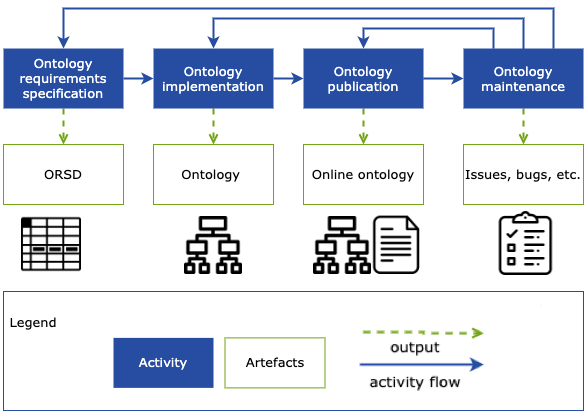
\includegraphics[width=0.6\linewidth]{figures/chp4-2_lot.png}
\caption[LOT Methodology]{Workflow proposed by the LOT Methodology~\parencite{poveda2022lot}.}
\label{fig:chp4-2_lot}
\end{figure}

\noindent\textbf{Maintenance}
Finally, the last stage of the development process, maintenance, refers to ontology updates as new requirements are found and/or errors are fixed. The ontology presented in this work promotes the gathering of issues or new requirements through the use of issues in the ontology GitHub repository. Additionally, it provides control of changes, and the documentation enables access to previous versions. Further details are shown in \cref{sec:chp4_pub-main}.



\subsection{Requirements}
\label{sec:chp4_requirements}
%\ana{añadir requisitos en anexo?}
This section presents the purpose, scope, and requirements of the Conceptual Mapping Ontology. In addition, it also describes from where and how the requirements are extracted: analysing the mapping languages (presented as a comparative framework in \cref{sec:chp4_framework}) and the Mapping Challenges proposed by the community.

\subsubsection{Purpose and scope}

The Conceptual Mapping ontology aims at gathering the expressiveness of declarative mapping languages that describe the transformation of heterogeneous data sources into RDF. This ontology-based language settles on the assumption that all mapping languages used for the same basic purpose of describing data sources in terms of an ontology to create RDF, must share some basic patterns and inherent characteristics. Inevitably, not all features are common. As described in previous sections, some languages were developed for specific purposes, others extend existing languages to cover additional use cases, and others are in turn based in languages that already provide them with certain capabilities. The Conceptual Mapping ontology is designed to represent and articulate these core features, which are extracted from two sources: (i) the analysis of current mapping languages, and (ii) the limitations of current languages identified by the community. These limitations, proposed by the W3C Knowledge Graph Construction Community Group\footnote{\label{foot:kgc}\url{https://www.w3.org/community/kg-construct/}}, are referred to as Mapping Challenges\footnote{\label{foot:challenges}\url{https://w3id.org/kg-construct/workshop/2021/challenges.html}} and have been partially implemented by some languages. %Both sources are described throughout this section.

This ontology also presents some limitations. As shown in \cref{sec:chp2_declarative_kgc}, mapping languages can be classified into three categories according to the schema in which they are based: RDF-based, SPARQL-based and based on other schemes. The Conceptual Mapping is included in the first category and, as such, has the same inherent capabilities and limitations as RDF-based languages regarding the representation of the language as an ontology. This implies that it is feasible to represent their expressiveness, whereas reusing classes and/or properties or creating equivalent constructs. Languages based on other approaches usually follow schemas that make them relatable to ontologies. This can be seen in the correspondence between YARRRML and RML: RML is written in Turtle syntax. YARRRML~\parencite{Heyvaert2018yarrrml} is mainly used as a user-friendly syntax to facilitate the writing of RML rules. It is based on YAML, and can easily be translated into RML\footnote{\url{https://rml.io/yarrrml/matey/}}. 

Lastly, SPARQL-based languages pose a challenge. SPARQL is a rich and powerful query language~\parencite{perez2009semantics} to which these mapping languages add more capabilities (e.g., SPARQL-Generate, SPARQL-Anything). It has an innate flexibility and capabilities sometimes not comparable to the other languages. For this reason, representing every single capability and feature of SPARQL-based languages is out of the scope of this work. Given the differences of representation paradigm between RDF and SPARQL for creating mappings, it cannot be ensured that the Conceptual Mapping covers all possibilities that a SPARQL-based language can, and as such, is considered a limitation.


\subsubsection{Mapping Challenges}
\label{sec:chp4_mapping_challenges}

Following its inception, the W3C Knowledge Graph Construction Community Group\cref{foot:kgc} defined a series of challenges for mapping languages based on the experience of members in using declarative mappings\cref{foot:challenges}. These challenges are a summary of the limitations of current languages. They have been partially addressed independently in some of the analyzed languages, such as RML~\parencite{delva2021rml-fields,iglesias2023rml} and ShExML~\parencite{garcia2021shexml-challenges}. These challenges are summarized as follows:

\begin{itemize}
    \item \textbf{[C1] Language Tags and Datatype.} It refers to dynamically building language tags [C1a] and datatypes [C1b], that is, from data rather than as constant values.
    \item \textbf{[C2] Iterators.} This challenge addresses the need to access data values 'outside' the iteration pattern [C2a], especially in \textcolor{black}{some tree-like data sources such as JSON}; and iterating over multi-value references [C2b].
    \item \textbf{[C3] Multi-value References.} It discusses how languages  handle data fields that contain multiple values [C3a], their datatypes and associated language tags [C3b].
    \item \textbf{[C4] RDF Collections and Containers.} This challenge addresses the need to handle RDF collections and containers.
    \item \textbf{[C5] Joins.} It refers to joining resources with zero join conditions [C5a] and joining literals instead of IRIs [C5b].
\end{itemize} 


\subsubsection{Conceptual Mapping Requirements}
\label{sec:chp4_cm-reqs}

In order to extract the requirements that serve as the basis for the development of the Conceptual Mapping ontology, we take as input the analysis from the comparison framework (\cref{sec:chp4_framework}) and the Mapping Challenges (\cref{sec:chp4_mapping_challenges}) described previously and the expertise of the authors. From a combination of their features, we extract 30 requirements. These requirements are expressed as facts, and are available in the ontology repository and portal\footnote{\url{https://oeg-upm.github.io/Conceptual-Mapping/requirements/requirements-core.html}}. Each requirement has a unique identifier, its provenance (comparison framework or mapping challenge id) and the corresponding constructs in the ontology. The constructs are written in Turtle, and lack cardinality restrictions for the sake of understandability. These requirements are tested with Themis, and its corresponding tests include these restrictions. More details on the evaluation of the requirements are provided in \cref{sec:chp4_cm-eval}. 

The requirements gathered range from general-purpose to fine-grained details. The general-purpose requirements refer to the basic fundamental capabilities of mappings, e.g., to create the rules to generate RDF triples (cm-r8) from reference data sources (cm-r7). The requirements with the next level of detail involve some specific restrictions and functionalities, e.g. to indicate the specific type (whether they are IRIs, Blank nodes, etc.) of subjects (cm-r16), predicates (cm-r17), objects (cm-r18), named graphs (cm-r19), datatypes (cm-r20) and language tags (cm-r21); the possibility of using linking conditions (cm-r23) and functions (cm-r15). Finally, some requirements refer to specific details or features regarding the description of data sources (e.g. cm-r4, cm-r6) and transformation rules (e.g. cm-r14, cm-r22, cm-r25).

Not all the observed features in the comparison framework have been added to the set of requirements. Some features are really specific, and supported by a minority of languages, sometimes only one language. As a result, we selected the (really) detailed features in these requirements to build the core specification of the Conceptual Mapping when they tackled the basic functionalities of the language. The rest of the details are left to be included as extensions. This differentiation and the modeling criteria is explained further in \cref{sec:chp4_implementation}.










\subsection{Implementation}
\label{sec:chp4_implementation}

This section describes in detail the activities and tasks carried out to implement the ontology, that consists in the conceptualization of the model, the encoding in a formal language, and the evaluation to fix errors, inconsistencies, and ensure that it meets the requirements. Additionally, an example of the ontology's use is presented at the end of the section.



\subsubsection{Ontology Conceptualization}




\begin{sidewaysfigure*}[]
    \centering
    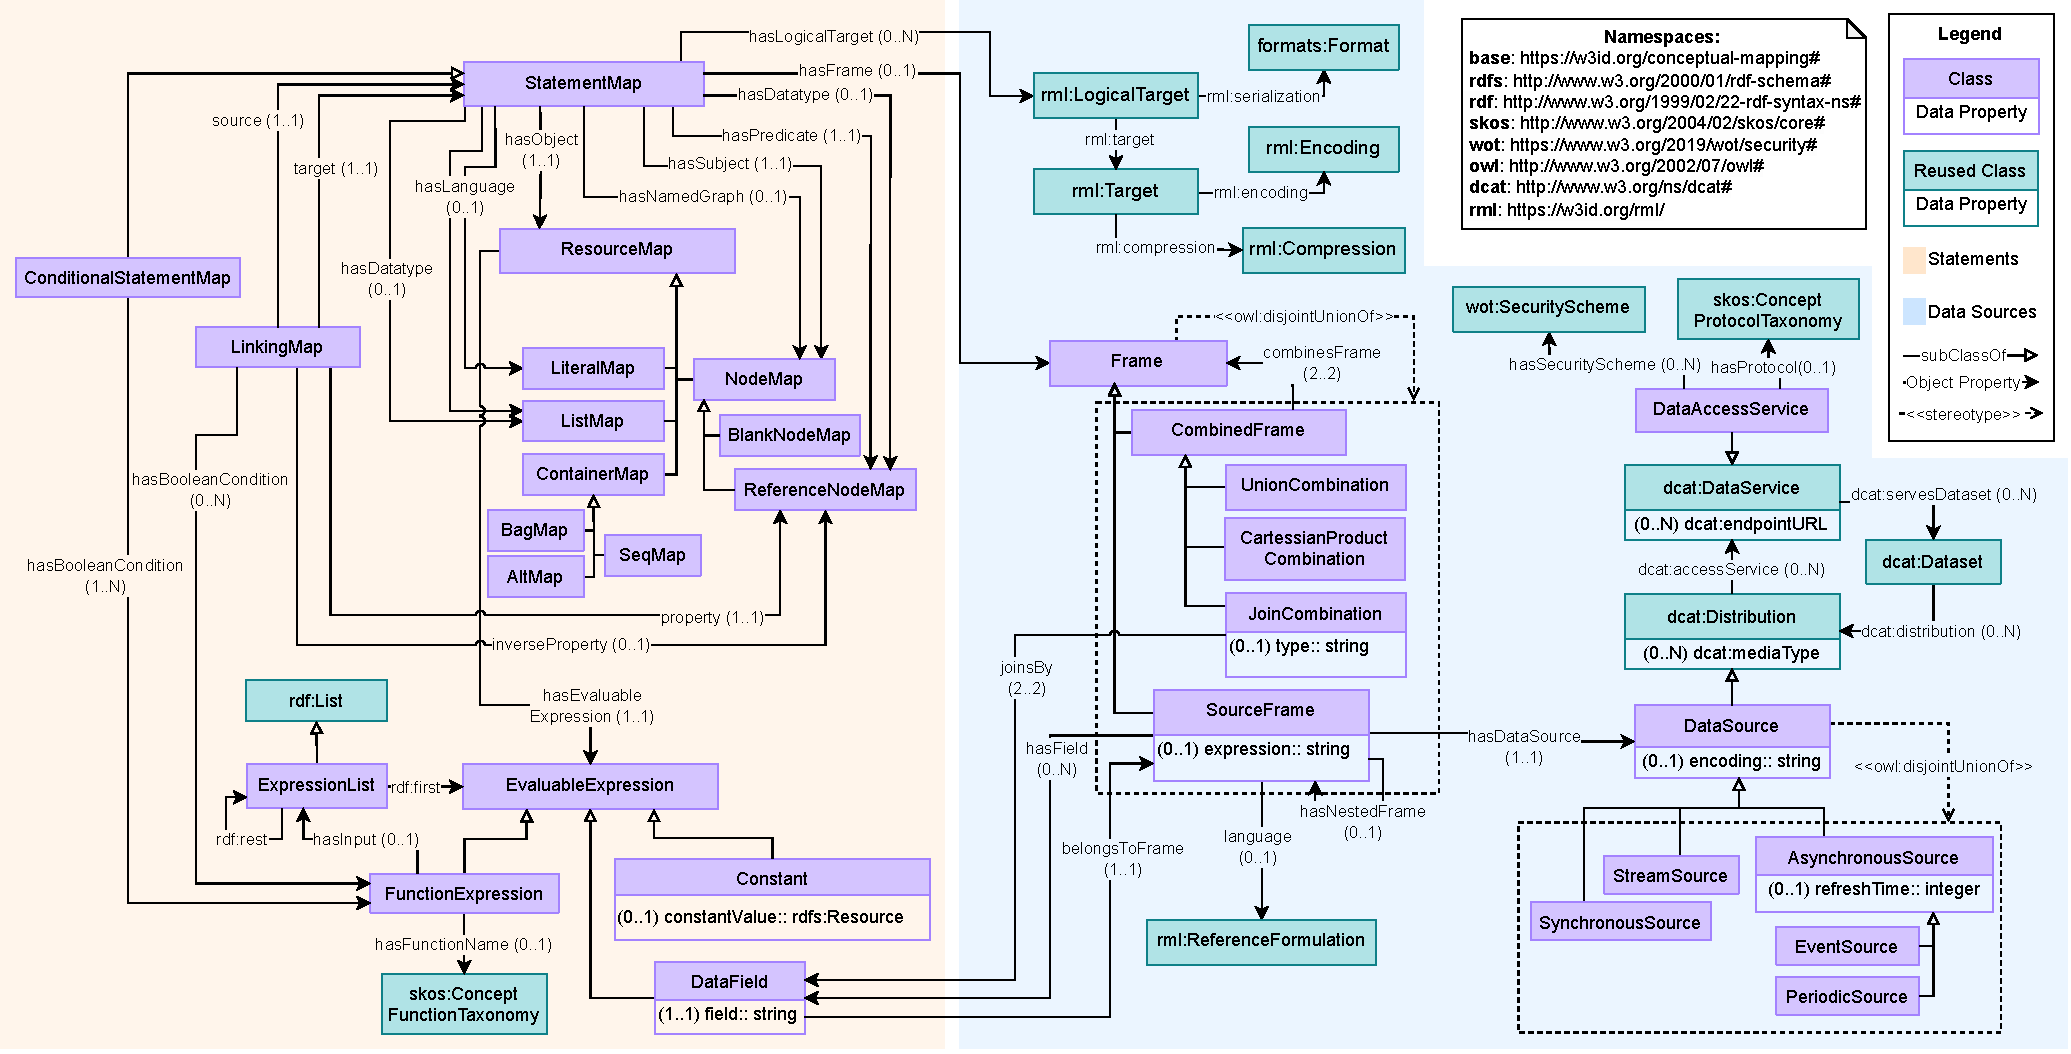
\includegraphics[width=1\linewidth]{figures/chp4-2_cm_diagram.pdf}
    \caption[Conceptual Mapping ontology overview]{Visual representation of the Conceptual Mapping ontology created using the Chowlk visual notation~\parencite{feria2022chowlk}.}
    \label{fig:chp4-2_cm_diagram}
\end{sidewaysfigure*}

\textcolor{black}{The ontology's conceptualization is built upon the requirements extracted from experts experience, a thorough analysis of the features and capabilities of current mapping languages presented as a comparative framework; and the languages' limitations discussed by the community and denoted as Mapping Challenges. The resulting ontology model is depicted in \cref{fig:chp4-2_cm_diagram}. This model represents the core specification of the Conceptual Mapping ontology that contains the essential features to cover the requirements. Some detailed features are also included when considered important to the language expressiveness, or needed for the language main functionality. Other detailed features are considered as extensions, as explained further in \cref{sec:chp4_cm-extensions}. For description purposes, we divide the ontology into two parts, \textit{Statements} and \textit{Data Sources}, that compose the core model. These two parts, when not used in combination, cannot describe a complete mapping. For that reason they are not separated into single modules. } 

\noindent\paragraph{\textbf{Data sources.}} A data source (\texttt{DataSource}) describes the source data that will be translated. For this section, the Data Catalog (DCAT) vocabulary~\parencite{albertoni2020dcat2} has been reused. \texttt{DataSource} is a subclass of \texttt{dcat:Distribution}, which is a specific representation of a dataset (\texttt{dcat:Dataset}), defined as ``data encoded in a certain structure such as lists, tables and databases''. A source can be a streaming source (\texttt{StreamSource}) that continuously generates data, a synchronous source (\texttt{SynchronousSource}) or an asynchronous source (\texttt{AsynchronousSource}). Asynchronous sources, in turn, can be event sources (\texttt{EventSource}) or periodic sources (\texttt{Periodic Source}). The details of the data source access are represented with the data access service class (\texttt{Data AccessService}), which in turn is a subclass of \texttt{dcat:DataService}. This class represents a collection of operations that provides access to one or more datasets or data processing functions, i.e., a description of how the data is accessed and retrieved. The data access service optionally has a security scheme (e.g., OAuth2, API Key, etc.) and an access protocol (e.g., HTTP(s), FTP, etc.).

Data properties in the \texttt{dcat:Dataset}, \texttt{dcat:Distribution} and \texttt{dcat:DataService} classes may be reused according to the features that may be represented in each mapping language, e.g. \texttt{dcat:endpointURL},  \texttt{dcat:accessURL} and \texttt{dcat:endpointDescrip\-tion}. A data access service is related to a security scheme. The class \texttt{wot:Securi\-tyScheme} (from the Web of Things (WoT) Security ontology\footnote{\label{foot:wotsec}\url{https://www.w3.org/2019/wot/security}}) has been reused. This class has different types of security schemes as subclasses and includes properties to specify the information on the scheme (e.g. the encryption algorithm, the format of the authentication information, the location of the authentication information). The security protocol \texttt{hasProtocol} has as set of predefined values that have been organized as a SKOS concept scheme. It contains almost 200 security protocols, e.g., HTTP(s), JDBC, FTP, GEO, among others. This SKOS list can be extended according to the users' needs by adding new concepts. 

In order to represent the fragments of data that are referenced in a statement map, the class \texttt{Frame} has been defined. They are connected with the property \texttt{hasFrame}. A frame can be a \texttt{SourceFrame} (base case) or a \texttt{CombinedFrame}, the latter representing two source frames or combined frames that are combined by means of a join (\texttt{JoinCombination}), a union (\texttt{UnionCombination}) or a cartessian product (\texttt{Cartessi\-anProductCombination}). 

A source frame corresponds to a data source (with \texttt{hasDataSource}) and defines which data is retrieved from the source and how it is fragmented (with \texttt{expression}). Among others, JSONPaths, XPaths, queries, or regular expressions can be expressed with this feature. \textcolor{black}{The language of the expression is defined with \texttt{language}, which domain is the reused class from RML \texttt{rml:ReferenceFormulation}}. A source frame may be related to another source frame with  \texttt{hasNest\-edFrame}, e.g. a frame is accessed firstly with a SPARQL query, and their results as a CSV file with this property. A source fragment may refer to many data fields (with \texttt{hasField}, which is the inverse property of \texttt{belongsToFrame}).

The desired output of the statements that are to be generated can be described with the imported \texttt{rml:LogicalTarget}, referenced by the optional property \texttt{hasLogicalTarget}. A \texttt{rml:LogicalTarget} specifies which RDF serialisation the output should be encoded (\texttt{rml:serialization}), and the referred \texttt{rml:Target}. 
The \texttt{rml:Target} indicates how the output target can be accessed,
and can describe: (i) the compression format for the RDF output (\texttt{rml:compression}) and, if so, how e.g., GZip,
and (ii) the encoding (\texttt{rml:encoding}), e.g., UTF-8.

\noindent\paragraph{\textbf{Statements.}} The central class of this section is the \texttt{StatementMap}, which represents a rule that defines for a triple its subject (\texttt{hasSubject}), predicate (\texttt{hasPredicate}), and object (\texttt{hasObject}). Optionally, it can also specify the object datatype (\texttt{hasDatatype}), language (\texttt{hasLanguage}) and assigned named graph (\texttt{hasNamedGraph}). Therefore, statement maps are similar to RDF statements as both of them are comprised by a subject, predicate and object. In statement maps, objects are resources (\texttt{ResourceMap}), and subjects and predicates are more specific, certain subclasses of the resource map: predicates are reference node maps (\texttt{ReferenceNodeMap}) that represent resources with an IRI, i.e., ontology properties. Subjects are node maps (\texttt{NodeMap}) that may be blank nodes (\texttt{Blank Node}) or also reference node maps. An object may be a literal (\texttt{LiteralMap}), a blank node, a container (\texttt{ContainerMap}) or a collection that defines a list (\texttt{ListMap}). The language is expressed as a literal, and the datatype is also a resource with an IRI, i.e. a reference node map.

Resource maps are expressed with an evaluable expression (\texttt{EvaluableExpression}) that may be a constant value (\texttt{Constant}), a function expression (\texttt{FunctionExpression}), or a data field (\texttt{DataField}) that belongs to some data source fragment (\texttt{belongsToFrame}). For function expressions, the function name (\texttt{hasFuntionName}) is taken from a set of predefined names organized in a SKOS concept scheme. This SKOS list can be extended according to the users' needs by adding new concepts for functions that have not been defined. Recursion in this function expression is represented through its input (\texttt{hasInput}) as an expression list (\texttt{ExpressionList}). Expression lists have been represented as a subclass of RDF lists (\texttt{rdf:List}), and the properties (\texttt{rdf:first}) and (\texttt{rdf:rest}) have been reused. Expression lists may have nested expression lists inside.


A special case of a statement map is a conditional statement map (\texttt{ConditionalSta\-tementMap}), a statement map that must satisfy a condition for the triples to be generated. The condition (\texttt{hasBooleanCondition}) is a function expression (e.g. if a value from a field called ``present'' is set to ``False'', the statement is not generated). Another relevant class is the linking map (\texttt{LinkingMap}), that enables linking subjects from a source (\texttt{source}) and a target (\texttt{target}) statement maps, i.e., two resources are linked and triples are generated if a linking condition is satisfied. Similarly to the conditional statement map, this condition is represented as a function expression.

\subsubsection{Ontology Design Patterns}
The following ontology design patterns \textcolor{black}{have been applied in the conceptualization as they are common solutions to the problem of representing taxonomies and linked lists}:
\begin{itemize}
    \item The SKOS vocabulary has been reused to represent some coding schemes such as the protocol taxonomy and the function taxonomy. \textcolor{black}{The design pattern consists on having an instance of} \texttt{skos:ConceptScheme} for each taxonomy, then each concept or term in the taxonomy, \texttt{skos:Concept}, is related to the corresponding concept scheme through the property \texttt{skos:inScheme}. The class that uses the taxonomy is then related to \texttt{skos:Concept} through an object property, e.g., class \texttt{DataAccessSer\-vice} and object property \texttt{hasProtocol}.
    \item The class \texttt{ExpressionList} uses the \textcolor{black}{design} pattern for lists developed in RDF where the properties \texttt{rdf:first} and \texttt{rdf:rest} are used to represent a linked list. The base case (first) is an evaluable expression whereas the rest of the list is (recursively)  an \texttt{ExpressionList}.
\end{itemize}

\subsubsection{Ontology evaluation}
\label{sec:chp4_cm-eval}


The ontology, implemented in OWL with Protégé, has been evaluated in different ways to ensure that it is correctly implemented, has no errors, inconsistencies or pitfalls, and meets the requirements.

\noindent\paragraph{\textbf{Reasoner.}} We used the reasoner Pellet in Protégé to look for inconsistencies in the model, and the results showed no errors.

\noindent\paragraph{\textbf{OOPS!.}}~\parencite{poveda2014oops} This tool was used to identify modeling pitfalls in the ontology. We executed the tool several times to fix the pitfalls, until there were no important ones. Currently, the results of OOPS! show pitfalls from the reused ontologies, but none important for the newly created terms and axioms. One minor pitfall is returned, P13, regarding the lack of inverse relationships, which we consider that are not  needed in the ontology. The rest of the pitfalls are as follows: P08 (missing annotations) from DCTERMS; P11 (missing domain or range in properties) for DCTERMS, DCAT and SKOS; and P20 (missing ontology annotations) for DCAT.

\noindent\paragraph{\textbf{Themis.}}~\parencite{fernandez2021themis} Themis is a tool able to evaluate whether the requirements are implemented in the ontology. To that end, the requirements must be provided in a specific syntax or described with the Verification Test Case (VTC) ontology\footnote{\url{https://albaizq.github.io/test-verification-ontology/OnToology/ontology/verification-test-description.ttl/documentation/index-en.html}}. The requirements of the Conceptual Mapping were translated to create the corresponding tests, and were tested in the tool with success. The requirements and associated test along with the complete set of tests annotated with the VTC ontology are available in the GitHub repository\footnote{\url{https://github.com/oeg-upm/Conceptual-Mapping/tree/main/requirements}}.

\noindent\paragraph{\textbf{FOOPS!.}}~\parencite{garijo2021foops} Additionally, we tried running FOOPS! to check the FAIRness of the ontology, resulting in 73\%, which is acceptable. To improve the score, the ontology should be added to a registry and have more metadata describing it, and use a persistent base IRI. 

With these evaluations, we can conclude that the ontology is correctly encoded and implemented, and that it meets the requirements specified in \cref{sec:chp4_requirements}. 



\subsection{Publication and Maintenance}
\label{sec:chp4_pub-main}

In order to publish the ontology, the first step required is to create the ontology documentation. We used Widoco~\parencite{garijo2017widoco}, integrated inside the OnToology~\parencite{alobaid2019automating} system, to automatically generate and update the HTML documentation every time there is a commit in the GitHub repository where the ontology is stored. This documentation contains the ontology metadata, links to the previous version, a description of the ontology, the diagram, and detailed examples of the capabilities of the language. It is published using a W3ID URL\cref{foot:cmlink} and under the CC BY-SA 4.0 license.

The HTML documentation is not the only documentation resource provided. An overview of all resources is provided in the ontology portal\cref{foot:cmportal}. This portal shows in a table the ontologies associated with the Conceptual Mapping ontology. For now, the core (Conceptual Mapping) and an extension to describe CSV files in detail (Conceptual Mapping - CSV Description) are available. For each ontology, links to the HTML documentation, the requirements, the GitHub repository, the Issue Tracker, and the releases are provided. 

The maintenance is supported by the Issue Tracker\footnote{\url{https://github.com/oeg-upm/Conceptual-Mapping/issues}}, where proposals for new requirements, additions, deletions or modifications can be added as GitHub issues. This approach allows authors to review the proposals and discuss their possible implementation.



\subsection{Extensions}
\label{sec:chp4_cm-extensions}
The Conceptual Mapping ontology has been designed as a core ontology. However, as time passes, new requirements may emerge. In order to include these new requirements, new modules of the Conceptual Mapping ontology shall be developed. It is worth mentioning that this is a common practice for ontologies, which is highly suitable for adapting an existing ontology to new scenarios, by ontology modules specialized for a specific set of requirements. A clear example of this is the SAREF ontology\footnote{\url{https://saref.etsi.org/}}, that has a core module\footnote{\url{https://saref.etsi.org/core/v3.1.1/}} and then specific extensions\footnote{\url{https://saref.etsi.org/extensions.html}} for certain domains, such as energy (SAREF4ENER) or buildings (SAREF4BLDG) among others. For the Conceptual Mapping we present two extensions: for allowing a more detailed description of CSV files, and for generating RDF-star graphs.


\begin{figure}[!t]
\centering
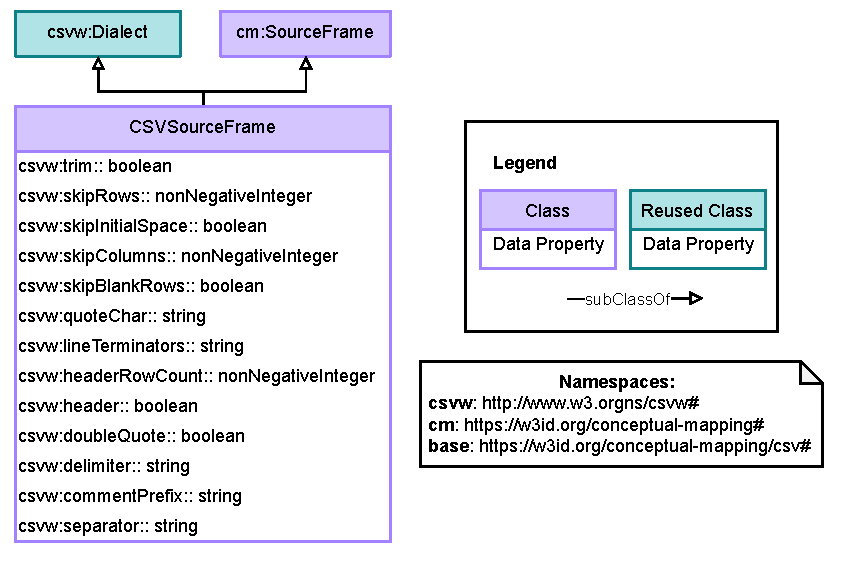
\includegraphics[width=0.8\linewidth]{figures/chp4-2_cm-csv.pdf}
\caption[CM-CSV module]{Conceptualization of the CM-CSV module following the Chowlk visual notation~\parencite{feria2022chowlk}.}
\label{fig:chp4-2_cm-csv}
\end{figure}


\subsubsection{CSV description: CM-CSV}
The core module of the Conceptual Mapping includes limited possibilities for describing CSV files in depth. The extension CM-CSV\footnote{\url{https://w3id.org/conceptual-mapping/csv}} provides extended features to this end. Thus, the CSVW~\parencite{Tennison2015csvw} proposal has been blended as an ontology module linked to the core Conceptual Mapping ontology. The class \texttt{CSVSourceFrame} is created as a subclass of \texttt{SourceFrame} and \texttt{csvw:Dialect} to inherit their characteristics. This module is depicted in \cref{fig:chp4-2_cm-csv}. Thus, this extension allows to describe CSV characteristics such as if the file contains headers (\texttt{csvw:header}), its delimiter (\texttt{csvw:delimiter}), separator (\texttt{csvw:separator}), among many others. 

\subsubsection{RDF-star generation: CM-star}
\label{sec:chp4_cm-star}
RDF-star~\parencite{hartig2017foundations} was recently proposed as a compact alternative for reification in RDF. It extends the RDF syntax introducing the notion of \textit{Quoted triples}, i.e. triples that can be placed in the position of objects and/or subjects. These triples can be inserted in the graph outside the quoted triple (i.e. they are \textit{asserted}), or appear only inside another triples (i.e. they are \textit{non-asserted}).

RDF-star has quickly gained popularity, leading
to its adoption by a wide range of systems~\footnote{\url{https://w3c.github.io/rdf-star/implementations.html}} (e.g., Apache Jena~\footnote{\url{https://jena.apache.org}}, Oxigraph~\parencite{oxigraph}) and the formation of the RDF-star Working Group\footnote{\url{https://www.w3.org/groups/wg/rdf-star}}. 
Regarding mapping languages, SPARQL-Anything is able to generate RDF-graphs as it natively implements the updates from Apache Jena; RML was extended for this purpose with the RML-star module~\parencite{iglesias2022rmlstar,delva2021rml-star,iglesias2023rml} (explained in detail in \cref{sec:chp4_rml_star}), as well as R2RML-star~\parencite{sundqvist2022extending}.

\begin{figure}[!t]
\centering
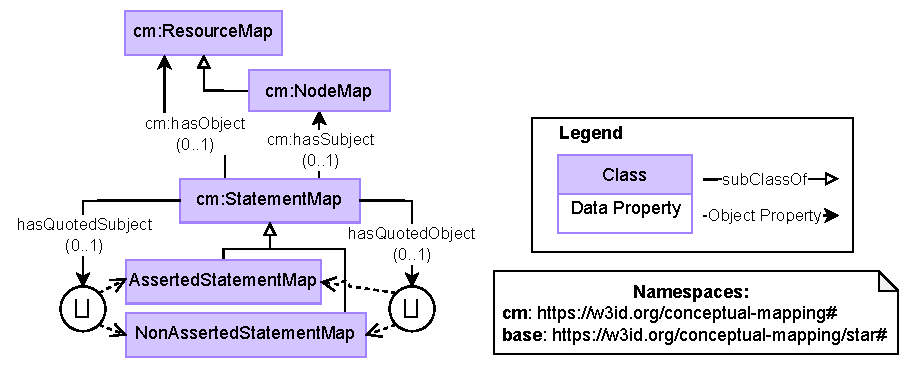
\includegraphics[width=0.9\linewidth]{figures/chp4-2_cm-star.pdf}
\caption[CM-star module]{Conceptualization of the CM-star module following the Chowlk visual notation~\parencite{feria2022chowlk}.}
\label{fig:chp4-2_cm-star}
\end{figure}




As a result, we developed a module to cover this new feature. The Conceptual Mapping implements the RDF-star graph generation adopting the recursive nature of quoted triples in the CM-star module\footnote{\url{https://w3id.org/conceptual-mapping/star}}. \cref{fig:chp4-2_cm-star} represents the overview of this module. Two subclasses of \texttt{StatementMap} are created to denote asserted (\texttt{AssertedStatementMap}) and non-asserted (\texttt{NonAssertedStatementMap}) statement maps. These statements can be quoted as subjects and objects with the properties \texttt{hasQuotedSubject} and \texttt{hasQuotedObject} respectively. The range of these properties is the union of the introduced statement subclasses. This extension enables potentially an infinite number of quoted statements, as the RDF-star specification indicates~\parencite{hartig2023rdf}. 



\subsection{Ontology usage example}\label{sec:cm_example} 



\begin{figure}[t!]
    \centering
    \begin{subfigure}[b]{0.45\linewidth}
        \centering
    	\includegraphics[width=1\linewidth]{figures/chp4-2_example_ont}
    	\caption{Example reference ontology that represents the classes \texttt{City} and \texttt{Location}, linked by the property \texttt{eg:location}.}
    	\label{fig:chp4-2_chp4_ex_onto}
    \end{subfigure}
    \begin{subfigure}[b]{0.28\linewidth}
        \centering
    	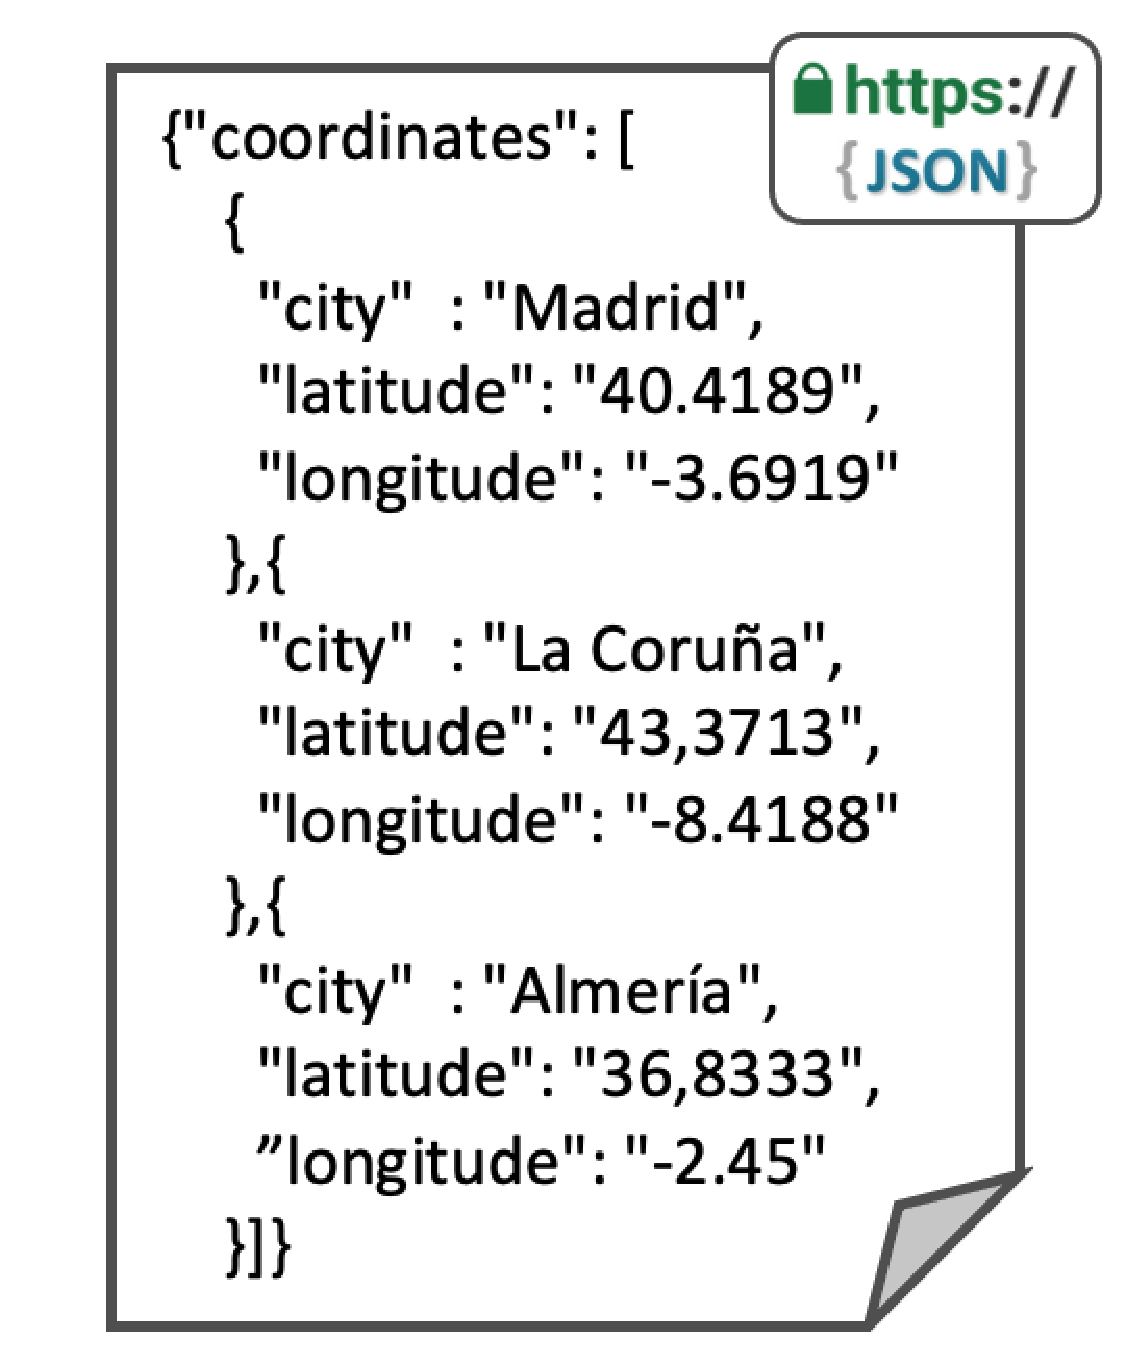
\includegraphics[width=1\linewidth]{figures/chp4-2_example_json}
    	\caption{Example input JSON file ```coordinates.json".}
    	\label{fig:chp4-2_chp4_ex_json}
    \end{subfigure}
    \begin{subfigure}[b]{0.7\linewidth}
        \centering
    	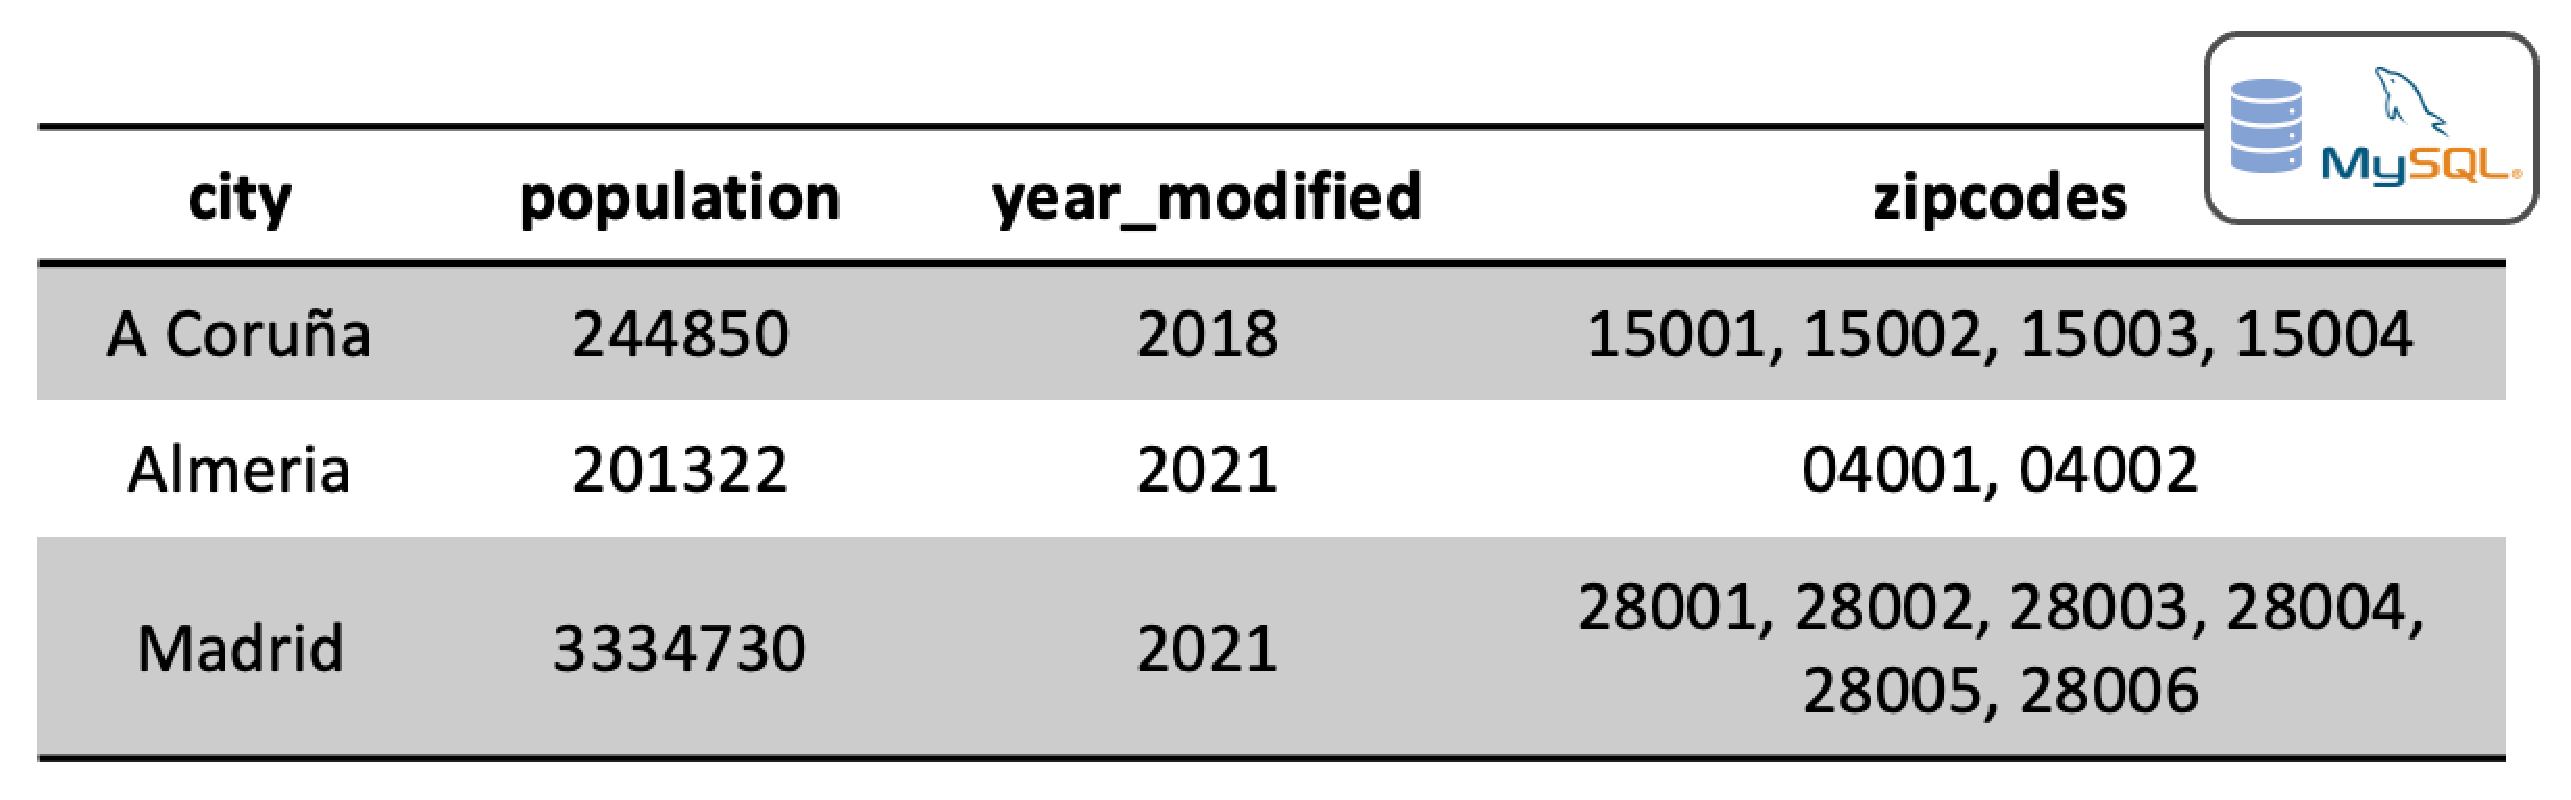
\includegraphics[width=1\linewidth]{figures/chp4-2_example_rdb}
    	\caption{Example input MySQL table ```cities".}
    	\label{fig:chp4-2_chp4_ex_rdb}
    \end{subfigure}
    \caption[Example data and ontology about cities for CM mapping]{Input source data and reference ontology that represents information on cities and their location.}
    \label{fig:chp4-2_chp4_ex_input}
\end{figure}



%\ana{no sé si dejar esto o rehacer y poner de drugs4covid, para que no sean datos de juguete. O si acaso poner que sea un use case, eso requeriría de hacer el mapping también en otros lenguajes. Por ahora dejar como está}

This section builds a mapping in three steps (data sources in \cref{lst:chp4_cm_sources}, triples in \cref{lst:chp4_cm_spo} and special statements in \cref{lst:chp4_cm_general}) to represent how the proposed language can describe data with different features. The mapping uses the data sources ``coordinates.json" (\cref{fig:chp4-2_chp4_ex_json}) and ``cities" (\cref{fig:chp4-2_chp4_ex_rdb}) as input and the ontology depicted in  \cref{fig:chp4-2_chp4_ex_onto} as reference, to create the output RDF shown in \cref{lst:chp4_output}. 
%Additionally, \cref{appendix2}\ana{APENDIX!!} contains a second example to illustrate different features than the ones represented in the example of this section, to provide more insights about the expressiveness of this language.

\begin{captionedlisting}{lst:chp4_output}{Expected RDF output for the data sources and the ontology in \cref{fig:chp4-2_chp4_ex_input}.}
\centering
{\begin{lstlisting}[]
<http://ex.com/loc/40.4189--3.6919> a eg:Location ;
	eg:lat "40.4189"^^xsd:decimal ;
	eg:long "-3.6919"^^xsd:decimal .
<http://ex.com/loc/43.3713--8.4188> a eg:Location ;
	eg:lat "43.3713"^^xsd:decimal ;
	eg:long "-8.4188"^^xsd:decimal .
<http://ex.com/loc/36.8333--2.45> a eg:Location ;
	eg:lat "36.8333"^^xsd:decimal ;
	eg:long "-2.45"^^xsd:decimal .
<http://ex.com/city/ACoruña> a eg:City ;
	eg:zipcode 15001, 15002, 15003, 15004 ;
	eg:location <http://ex.com/loc/43.3713--8.4188> .
<http://ex.com/city/Almería> a eg:City ;
	eg:zipcode 04001, 04002 ;
	eg:population 201322 ;
	eg:location <http://ex.com/loc/36.8333--2.45> .
<http://ex.com/city/Madrid> a eg:City ;
	eg:zipcode 28001, 28002, 28003, 28004, 28005, 28006;
	eg:population 3334730 ;
	eg:location <http://ex.com/loc/40.4189--3.6919> .
\end{lstlisting}}
\end{captionedlisting}

\noindent\paragraph{\textbf{Data sources.}} \cref{lst:chp4_cm_sources} shows the description of the json file ``coordinates.json" indicating the protocol from the SKOS concept scheme (\texttt{cmp:https}), media type (``application/json"), JSONPath to extract data, access URL  ``https://ex.com/geodata/coordi\-nates.json", and  fields that are going to be used in the transformation. There is no security scheme. The MySQL table ``cities" also has no security scheme, the protocol needed is \texttt{cmp:jdbc}, the database access is specified in the endpoint URL, and the table as an SQL query. The fields are also specified, with the special case of ``zipcodes" that needs a \texttt{cm:hasNestedFrame} to extract multiple values inside the field.

\begin{captionedlisting}{lst:chp4_cm_sources}{Description with the Conceptual Mapping of two data sources (a JSON file and a relational database), their access and fields.}
\centering
{\begin{lstlisting}[language=concm,firstnumber=1]
# Locations
:FrameLoc a cm:SourceFrame;
  cm:expression "$\dollar$.coordinates[*]";
  cm:language ql:JSONPath ;
  cm:hasField :lat;
  cm:hasField :long;
  cm:hasField :loc_city;
  cm:hasDataSource [ a cm:SynchronousSource;
    dcat:mediaType "text/json";
    dcat:accessService [
      cm:hasProtocol cmp:https;
      dcat:endpointURL "https://ex.com/geodata/coordinates.json" 
      cm:hasSecurityScheme [ a wotsec:NoSecurityScheme; ];
    ] ;
  ] .

:lat a cm:DataField ; cm:field "$\dollar$.latitude" .
:long a cm:DataField ; cm:field "$\dollar$.longitude" .
:loc_city a cm:DataField; cm:field "$\dollar$.city" .

# Cities
:FrameCities a cm:SourceFrame ;
  cm:expression "SELECT * FROM cities;";
  cm:hasField :c_city;
  cm:hasField :population;
  cm:hasField :year;
  cm:hasNestedFrame [
    cm:expression "$\dollar$.zipcodes[*]";
    cm:hasField :zipcode ];
  cm:hasDataSource [ a cm:SynchronousSource;
    dcat:mediaType "text/plain";
    dcat:accessService [
      cm:hasProtocol cmp:jdbc;
      dcat:endpointURL "jdbc:mysql://localhost:3306/citydb";
      cm:hasSecurityScheme [a wotsec:NoSecurityScheme;] ].

:c_city a cm:DataField; cm:field "city" .
:population a cm:DataField; cm:field "population" .
:year a cm:DataField; cm:field "year_modified" .
:zipcode a cm:DataField cm:field "zipcodes" .
\end{lstlisting}}
\end{captionedlisting}

%\noindent{\textbf{Locations.}} Sarah is working at the National Geographic Institute from Spain, and manages everyday information about places and locations. She wants to create a knowledge graph with the geographical data that she usually manages. She starts writing a mapping (\cref{lst:uc1}) to represent cities from a local JSON file, \texttt{Venue.json} (\cref{lst:data_venues}). This data will be transformed into instances of the class \texttt{City}. 

\noindent\paragraph{\textbf{Statements.}} \cref{lst:chp4_cm_spo} contains the rules needed to create instances of the classes \texttt{eg:Location} and \texttt{eg:City}; and their following attributes: \texttt{eg:lat} and \texttt{eg:long} for the former; \texttt{eg:zipcode} for the latter. To correctly generate the URI for the instances of \texttt{eg:City}, a replace function inside a concatenate function is needed to (1) remove the blank spaces in the field ``city" and (2) add the field to the base URI ``http://ex.com/city/".

\begin{captionedlisting}{lst:chp4_cm_spo}{Description with the Conceptual Mapping of the creation of regular statements from the data sources described in \cref{lst:chp4_cm_sources}.}
\centering
{\begin{lstlisting}[language=concm,firstnumber=1]
# Locations
:SubjectLoc a cm:ReferenceNodeMap ;
  cm:hasEvaluableExpression [
    cm:hasFunctionName cmf:concat; 
    cm:hasInput ([cm:constantValue "http://ex.com/loc/"]    :lat [cm:constantValue "-" ] :long)].

:StatementLoc1 a cm:StatementMap ;
  cm:hasFrame :FrameLoc ;
  cm:subject :SubjectLoc ;
  cm:predicate [ a cm:ReferenceNodeMap; 
    cm:hasEvaluableExpression [cm:constantValue rdf:type ] ];
  cm:object [cm:hasEvaluableExpression [cm:constantValue eg:Location]].

:StatementLoc2 a cm:StatementMap ;
  cm:hasFrame :FrameLoc ;
  cm:subject :SubjectLoc ;
  cm:predicate [ a cm:ReferenceNodeMap; 
    cm:hasEvaluableExpression [cm:constantValue eg:lat]];
  cm:object [ a cm:Literal; cm:hasEvaluableExpression :lat];
  cm:hasDatatype [cm:hasEvaluableExpression xsd:decimal].

:StatementLoc3 a cm:StatementMap ;
  cm:hasFrame :FrameLoc ;
  cm:subject :SubjectLoc ;
  cm:predicate [ a cm:ReferenceNodeMap; 
    cm:hasEvaluableExpression [cm:constantValue eg:long]];
  cm:object [ a cm:Literal; cm:hasEvaluableExpression :long];
  cm:hasDatatype [ cm:hasEvaluableExpression xsd:decimal].
    
# Cities
:city_ns a cm:FunctionExpression ;
  cm:functionName cmf:replace ;
  cm:hasInput (c_city " " "")

:SubjectCities a cm:ReferenceNodeMap;
  cm:hasEvaluableExpression [
    cm:hasFunctionName cmf:concat; 
    cm:hasInput ([cm:constantValue "http://ex.com/city/"] :city_ns)].

:StatementCit1 a cm:StatementMap ;
  cm:hasFrame :FrameCities ;
  cm:subject :SubjectCities ;
  cm:predicate [ a cm:ReferenceNodeMap; 
    cm:hasEvaluableExpression [cm:constantValue rdf:type]];
  cm:object [ a cm:ReferenceNodeMap; 
    cm:hasEvaluableExpression  [cm:constantValue eg:City]] .

:StatementCit2 a cm:StatementMap ;
  cm:hasFrame :FrameCities ;
  cm:subject :SubjectCities ;
  cm:predicate [ a cm:ReferenceNodeMap; 
    cm:hasEvaluableExpression [cm:constantValue rdfs:label]];
  cm:object [ a cm:ReferenceNodeMap; 
    cm:hasEvaluableExpression  [cm:constantValue :c_city]] .
  cm:hasLanguage [ cm:hasEvaluableExpression [ cm:constantValue "es" ] ].

:StatementCit3 a cm:StatementMap ;
  cm:hasFrame :FrameCities ;
  cm:subject :SubjectCities ;
  cm:predicate [ a cm:ReferenceNodeMap; 
    cm:hasEvaluableExpression [cm:constantValue eg:zipcode] ];
  cm:object [ a cm:Literal;
    cm:hasEvaluableExpression [cm:constantValue :zipcode] ];
  cm:hasDatatype [ cm:hasEvaluableExpression xsd:integer ].
\end{lstlisting}}
\end{captionedlisting}


\noindent\paragraph{\textbf{Special statements.}} \cref{lst:chp4_cm_general} describes how a conditional statement and a linking rule are generated. This description is represented by means of functions. With the property \texttt{cm:hasBooleanCondition}, the conditional statement declares that the field \texttt{:year} has to be greater than 2020. The linking rule performs the link between the instances of \texttt{eg:City} and \texttt{eg:Location} with the predicate \texttt{eg:location}, using a distance metric (levenshtein function) that has to be greater then a threshold of ``0.75". 

\begin{captionedlisting}{lst:chp4_cm_general}{Conditional and linking rules described with the Conceptual Mapping that complement the data source description and regular statements described in \cref{lst:chp4_cm_sources} and \cref{lst:chp4_cm_spo}.}
\centering
{\begin{lstlisting}[language=concm,firstnumber=1]
:StatementCit4 a cm:ConditionalStatementMap ;
  cm:hasFrame :FrameCities ;
  cm:subject :SubjectCities ;
  cm:predicate [ a cm:ReferenceNodeMap; 
    cm:hasEvaluableExpression [cm:constantValue eg:population] ];
  cm:object [ a cm:Literal; 
    cm:hasEvaluableExpression  [cm:constantValue :population] ];
  cm:hasDatatype [ cm:hasEvaluableExpression xsd:integer];
  cm:hasBooleanCondition [
    cm:functionName cmf:greater_than ;
    cm:hasInput ( :year 2020 ) ] .

:LinkExp1 a cm:LinkingExpression ;
  cm:source :StatementCit1 ;
  cm:target :StatementLoc1 ;
  cm:property eg:location ;
  cm:hasBooleanCondition [
    cm:functionName cmf:greater_than ; 
    cm:hasInput ( :levfun 0.75 ) ] .

:levfun a cm:FunctionExpression ;
  cm:functionName cmf:levenshtein_distance ;    
  cm:hasInput (:c_city :loc_city) .
\end{lstlisting}}
\end{captionedlisting}









\section{Mapping Rules for RDF-star: RML-star}
\label{sec:chp4_rml_star}

%In the late years, the RDF-star~(\cite{hartig2017foundations}) approach for reification has gained popularity. Along with its expansions, different semantic web technologies have been updated to include this new syntax\footnote{\url{https://w3c.github.io/rdf-star/implementations}}. This section describes one of these updates related to building RDF-star graphs: RML-star. \ana{esto no liga del todo bien con lo anterior}



Making statements about statements in RDF has
posed a challenge almost since the inception of RDF.
The W3C RDF Primer~(\cite{manola2004rdf}) already included a description of the standard reification approach to tackle this issue.
Other alternatives were proposed over the years,
such as named graphs~(\cite{carroll2005namedgraphs}), N-ary relationships~(\cite{naryw3c2006}), singleton properties~(\cite{nguyen2014don}), RDF$^+$~(\cite{schueler2008querying}), and more recently, \mbox{RDF-star}~(\cite{hartig2017foundations}). 

RDF-star does not leverage the characteristics of RDF as the others proposals. Instead it extends the RDF syntax to introduce the notion of \texttt{embedded triples}. This approach is currently under development to become a W3C standard\footnote{\url{https://www.w3.org/groups/wg/rdf-star}}. 
As a consequence, an increasing number of semantic technologies are supporting this proposal\footnote{\url{https://w3c.github.io/rdf-star/implementations}}, which include triplestores (e.g. GraphDB, AnzoGraph) and programming libraries (e.g. Apache Jena, Oxigraph).

It is possible to construct reified RDF graphs using mappings with the reification approaches abovementioned, except for RDF-star. As this proposal extends the original RDF syntax, it requires mapping languages to adapt and evolve in order to construct RDF-star graphs. This chapter presents the extension of the RML language to enable the construction of RDF-star graphs, RML-star. We first introduce how reified RDF graphs can be constructed using RML with different reification approaches, and then we present RML-star. This proposal is validated with \mbox{Morph-KGC$^{star}$}, a KG construction engine that implements our proposal.

%This section describes popular reification approaches and shows how they can be used in RML and RML-star with a running example. 
%Standard reification and singleton properties are considered in Section \ref{sec:chp4_validation}, showing that \mbox{Morph-KGC$^{star}$} does not add any overhead in the time required to generate the \mbox{RDF-star} triples compared to them.

\subsection{Statements about statements in mapping rules}
\label{sec:chp4_reif_mappings}

We illustrate each reification alternative presented throughout this section with a running example that uses the data shown in \cref{lst:chp4_csv_star}.
It contains CSV data related to pole vault:
the vaulter (\texttt{PERSON}),
the height of the jump (\texttt{MARK}),
the date when the jump was performed (\texttt{DATE}) and
an identifier of the jump (\texttt{ID}).
The running example represents
that a person jumped some height on a specific date, i.e., it adds the metadata about ``date''
to the statement ``a person jumped some height''.

\noindent\hspace{0.15\linewidth}\begin{minipage}{\linewidth}
\begin{captionedlisting}{lst:chp4_csv_star}{Contents of the logical source \texttt{:marks} in CSV format.}
\centering
\begin{tabular}{c}
\hspace{3em}
{\begin{lstlisting}[basicstyle=\ttfamily\small,label={list:example1},columns=flexible]
ID  , DATE       , MARK ,   PERSON
1   , 2022-03-21 , 4.80 ,   Angelica
2   , 2022-03-19 , 4.85 ,   Katerina
\end{lstlisting}}
\end{tabular}
\end{captionedlisting}
\end{minipage}

\subsubsection{Reification with RML}

There are several reification approaches for RDF as presented in \cref{chp2_reification}, such as standard reification, singleton properties, N-ary relationships or named graphs. 
These approaches use strategies that add metadata to triples
without modifying the original RDF syntax.
Thus, they can be used with RML without any further modification. RML mapping rules enable the generation of blank nodes (required for the standard reification approach), dynamically generated predicates (required for the singleton properties approach) and named graphs (required for the named graphs approach). %\ana{si voy con todos, influye en el ejemplo de aquí abajo y en los use cases. En ese caso, quitar somef (demasiado grande el mapping, con semmeddb es suficiente)}

%\ana{probablemente en sota estarán explicados cada uno de los modelos, probablemente no haga falta ponerlos aquí también.}


\noindent\textbf{\textit{Standard Reification}}~(\cite{manola2004rdf}) was proposed in the W3C RDF Primer~(\cite{manola2004rdf}).
It assigns statements to unique identifiers (typically blank nodes) typed with \texttt{rdf:Statement} and described using the properties \texttt{rdf:subject}, \texttt{rdf:predicate} and \texttt{rdf:object}.
This way, the unique identifier representing the statement can be further annotated with additional statements. \cref{lst:chp4_res-std-reif} shows an example of standard reification for the data in \cref{lst:chp4_csv_star}, created with the RML mapping rules in \cref{lst:chp4_std-reif}. 
This mapping creates blank nodes in the subject with the \texttt{ID} data field, typed with \texttt{rdf:Statement}; and has three predicate object maps to generate the \texttt{rdf:subject}, \texttt{rdf:predicate}, \texttt{rdf:object} of the triples (\textit{An athlete jumps certain height}) and a predicate object map to annotate the statements with \texttt{:date} (\textit{in a specific date}).




\begin{minipage}{\linewidth}
\begin{captionedlisting}{lst:chp4_std-reif}{Example RML mapping using standard reification that transforms data in \cref{lst:chp4_csv_star}.}
\centering
\begin{multicols}{2}
{\begin{lstlisting}[basicstyle=\ttfamily\small,label={list:example1},columns=flexible]
<#TM> a rr:TriplesMap ;
  rml:logicalSource :marks ;
  rr:subjectMap [ 
    rml:reference "ID" ;
    rr:termType rr:BlankNode ;
    rr:class rdf:Statement  ] ;
  rr:predicateObjectMap [ 
    rr:predicate rdf:subject ;
    rr:objectMap [
      rr:template ":{PERSON}" ] ] ;
  rr:predicateObjectMap [ 
    rr:predicate rdf:predicate ;
    rr:object :jumps ] ;
  rr:predicateObjectMap [ 
    rr:predicate rdf:object ;
    rr:objectMap [
      rml:reference "MARK" ] ] ;
  rr:predicateObjectMap [ 
    rr:predicate :date ;
    rr:objectMap [
      rml:reference "DATE" ] ] .
\end{lstlisting}}
\end{multicols}
\end{captionedlisting}
\end{minipage}

\begin{minipage}{\linewidth}
\begin{captionedlisting}{lst:chp4_res-std-reif}{RDF triples generated by the mapping in \cref{lst:chp4_std-reif}.}
\centering
\begin{multicols}{2}
{\begin{lstlisting}[basicstyle=\ttfamily\small,label={list:example1},columns=flexible]
_:1 rdf:type      rdf:Statement .
_:1 rdf:subject   :Angelica .
_:1 rdf:predicate :jumps .
_:1 rdf:object    "4.80" .
_:1 :date         "2022-03-21" .
_:2 rdf:type      rdf:Statement .
_:2 rdf:subject   :Katerina .
_:2 rdf:predicate :jumps .
_:2 rdf:object    "4.85" .
_:2 :date         "2022-03-19" .
\end{lstlisting}}
\end{multicols}
\end{captionedlisting}
\end{minipage}



\noindent\textbf{\textit{Singleton Properties}}~(\cite{nguyen2014don}). This approach uses unique predicates linked with \texttt{rdf:singletonPropertyOf} to the original predicate. 
This unique predicate can then be annotated as the subject of additional statements. 
\cref{lst:chp4_res-sp-reif} shows the reified triples for the data in \cref{lst:chp4_csv_star} created with the RML mapping rules in \cref{lst:chp4_sp-reif}. 
It uses a singleton property dynamically generated with the \texttt{ID} data field for the property \texttt{:jumps} (\textit{An athlete jumps certain height}), annotated with \texttt{:date} (\textit{in a specific date}).


\begin{minipage}{\linewidth}
\begin{captionedlisting}{lst:chp4_sp-reif}{Example RML mapping using a singleton property that transforms data in \cref{lst:chp4_csv_star}.}
\centering
\begin{multicols}{2}
{\begin{lstlisting}[basicstyle=\ttfamily\small,label={list:example1},columns=flexible]
<#TM> a rr:TriplesMap ;
  rml:logicalSource :marks ;
  rr:subjectMap [ 
    rr:template ":{PERSON}" ] ;
  rr:predicateObjectMap [ 
    rr:predicateMap [
     rr:template ":jumps#{ID}" ] ;
    rr:objectMap [
      rml:reference "MARK" ] ] .
<#TM-SP> a rr:TriplesMap ;
  rr:logicalSource :marks ;
  rr:subjectMap [ 
    rr:template ":jumps#{ID}" ] ;
  rr:predicateObjectMap [ 
    rr:predicate rdf:singletonPropertyOf;
    rr:object :jumps ] ;
  rr:predicateObjectMap [ 
    rr:predicate :date ;
    rr:objectMap [
      rml:reference "DATE" ] ] .
\end{lstlisting}}
\end{multicols}
\end{captionedlisting}
\end{minipage}



\noindent\hspace{0.12\linewidth}\begin{minipage}{\linewidth}
\begin{captionedlisting}{lst:chp4_res-sp-reif}{RDF triples generated by the mapping in \cref{lst:chp4_sp-reif}.}
\centering
\begin{tabular}{c}
\hspace{4em}
{\begin{lstlisting}[basicstyle=\ttfamily\small,label={list:example1},columns=flexible]
:Angelica   :jumps#1  "4.80" .
:jumps#1    :date     "2022-03-21" .
:jumps#1    rdf:singletonPropertyOf :jumps .
:Katerina   :jumps#2  "4.85" .
:jumps#2    :date     "2022-03-19" .
:jumps#2    rdf:singletonPropertyOf :jumps .
\end{lstlisting}}
\end{tabular}
\end{captionedlisting}
\end{minipage}



\textit{\textbf{Named Graphs}}~(\cite{carroll2005namedgraphs}). This approach encloses each reified triple inside a unique named graph. This named graph can then be annotated with an additional triple. In \cref{lst:chp4_graph-reif} a graph is created for the triples that state the height of the jump (\texttt{:G} with the field \texttt{ID}) (\textit{An athlete jumps certain height}). A second graph contains the annotated triple and references the first graph (\texttt{:GA} with the field \texttt{ID}) (\textit{in a specific date}). The resulting RDF triples in TriG syntax\footnote{\url{https://www.w3.org/TR/trig/}} are shown in \cref{lst:chp4_res-graph-reif}.

\begin{minipage}{\linewidth}
\begin{captionedlisting}{lst:chp4_graph-reif}{Example RML mapping using named graphs that transforms data in \cref{lst:chp4_csv_star}.}
\centering
\begin{multicols}{2}
{\begin{lstlisting}[basicstyle=\ttfamily\small,label={list:example1},columns=flexible]
<#TM> a rr:TriplesMap ;
  rml:logicalSource :marks ;
  rr:subjectMap [ 
    rr:template ":{PERSON}" ;
    rr:graphMap [
      rr:template ":G{ID}" ] ] ;
  rr:predicateObjectMap [ 
    rr:predicateMap [
     rr:template ":jumps" ] ;
    rr:objectMap [
      rml:reference "MARK" ] ] .
<#TM-GA> a rr:TriplesMap ;
  rr:logicalSource :marks ;
  rr:subjectMap [ 
    rr:template ":{ID}" ;
    rr:graphMap [
      rr:template ":GA{ID}"] ] ;
  rr:predicateObjectMap [ 
    rr:predicate :date ;
    rr:objectMap [
      rml:reference "DATE" ] ] .
\end{lstlisting}}
\end{multicols}
\end{captionedlisting}
\end{minipage}

\noindent\hspace{0.12\linewidth}\begin{minipage}{\linewidth}
\begin{captionedlisting}{lst:chp4_res-graph-reif}{RDF triples generated by the mapping in \cref{lst:chp4_graph-reif}.}
\centering
\begin{tabular}{c}
\hspace{4em}
{\begin{lstlisting}[basicstyle=\ttfamily\small,label={list:example1},columns=flexible]
:G1  {:Angelica :jumps  "4.80" .}
:GA1 {:G1       :date   "2022-03-21" .}
:G2  {:Katerina :jumps#2  "4.85" .}
:GA2 {:G2       :date     "2022-03-19" .}
\end{lstlisting}}
\end{tabular}
\end{captionedlisting}
\end{minipage}


\textit{\textbf{N-Ary Relationships}}~(\cite{naryw3c2006}). This approach  converts a relationship into an instance that describes the relation, which can have attached both the main object and additional statements. The mapping shown in \cref{lst:chp4_nary-reif} creates instances of the relationship ``jump" with the field \texttt{ID}, which contain the date and height of the jump.  (\textit{An athlete jumps a jump with certain height and in a specific date}). 
The resulting RDF triples are shown in \cref{lst:chp4_res-nary-reif}.

\begin{minipage}{\linewidth}
\begin{captionedlisting}{lst:chp4_nary-reif}{Example RML mapping using a N-ary relationship that transforms data in \cref{lst:chp4_csv_star}.}
\centering
\begin{multicols}{2}
{\begin{lstlisting}[basicstyle=\ttfamily\small,label={list:example1},columns=flexible]
<#TM> a rr:TriplesMap ;
  rml:logicalSource :marks ;
  rr:subjectMap [ 
    rr:template ":{PERSON}" ] ;
  rr:predicateObjectMap [ 
    rr:predicateMap [
     rr:template ":jumps" ] ;
    rr:objectMap [
      rr:template ":Jump{ID}";
      rr:termType rr:IRI] ] .
<#TM-JUMP> a rr:TriplesMap ;
  rr:logicalSource :marks ;
  rr:subjectMap [ 
    rr:template ":Jump{ID}" ] ;
  rr:predicateObjectMap [ 
    rr:predicate :height ;
    rr:objectMap [
      rml:reference "MARK" ] ] ;
  rr:predicateObjectMap [ 
    rr:predicate :date ;
    rr:objectMap [
      rml:reference "DATE" ] ] .
\end{lstlisting}}
\end{multicols}
\end{captionedlisting}
\end{minipage}

\begin{minipage}{\linewidth}
\begin{captionedlisting}{lst:chp4_res-nary-reif}{RDF triples generated by the mapping in \cref{lst:chp4_nary-reif}.}
\centering
\begin{multicols}{2}
{\begin{lstlisting}[basicstyle=\ttfamily\small,label={list:example1},columns=flexible]
:Angelica  :jumps   :Jump1 .
:Jump1     :date    "2022-03-21" .
:Jump1     :height  "4.80" .
:Katerina  :jumps   :Jump2 .
:Jump2     :date    "2022-03-19" .
:Jump2     :height  "4.85" .
\end{lstlisting}}
\end{multicols}
\end{captionedlisting}
\end{minipage}




\subsubsection{Reification with RML-star}



We propose RML-star as an extension of RML to generate \mbox{RDF-star} graphs (\cref{fig:rml-star}). 
\mbox{RML-star} adds a new kind of term map, the \texttt{rml:StarMap}, that allows using triples maps to generate quoted triples. Following the \mbox{RDF-star} data model, star maps can only be used in subject and object maps. Star maps use the property \texttt{rml:quotedTri\-plesMap} to refer to the triples map that generates the quoted triples. This referenced triples map will also generate asserted triples, since it is a \texttt{rr:TriplesMap}. To enable the generation of quoted triples without asserting them, RML-star introduces \texttt{rml:NonAssertedTriplesMap} as a subclass of \texttt{rr:TriplesMap}. Non-asserted triples maps can be referred by \texttt{rml:quotedTriplesMap} to generate quoted triples, but they will be ignored when generating asserted triples.

The \mbox{RML-star} specification~(\cite{iglesias2022rmlstar}) provides a complete description of the language, it is published as a W3C Draft Community Report, and it is maintained by the W3C Knowledge Graph Construction Community Group\cref{foot:kgc}.
Both, the language and the specification are kept up to date reflecting the modifications in \mbox{RDF-star}.
For instance, the latest \mbox{RML-star} releases update the term ``embedded'' to ``quoted'',
according to the modifications in \mbox{RDF-star}.
This update renamed the property \texttt{rml:embeddedTriplesMap} 
%from a previous version\footnote{\url{https://kg-construct.github.io/rml-star-spec/20210706/}} to \texttt{rml:quotedTriplesMap}.
An example of an \mbox{RML-star} mapping rule for the data in \cref{lst:chp4_csv_star} is in \cref{lst:chp4_rml-star} which generates the \mbox{RDF-star} triples in \cref{lst:chp4_res-rml-star}. 
The mapping rules use a non-asserted triples map (\texttt{<\#jumpTM>}) within the subject map of a triples map (\texttt{<\#dateTM>}) which annotates quoted triples (\textit{An athlete jumps certain height}) with \texttt{:date} (\textit{in a specific date}).

\begin{figure*}[!t]
\centering
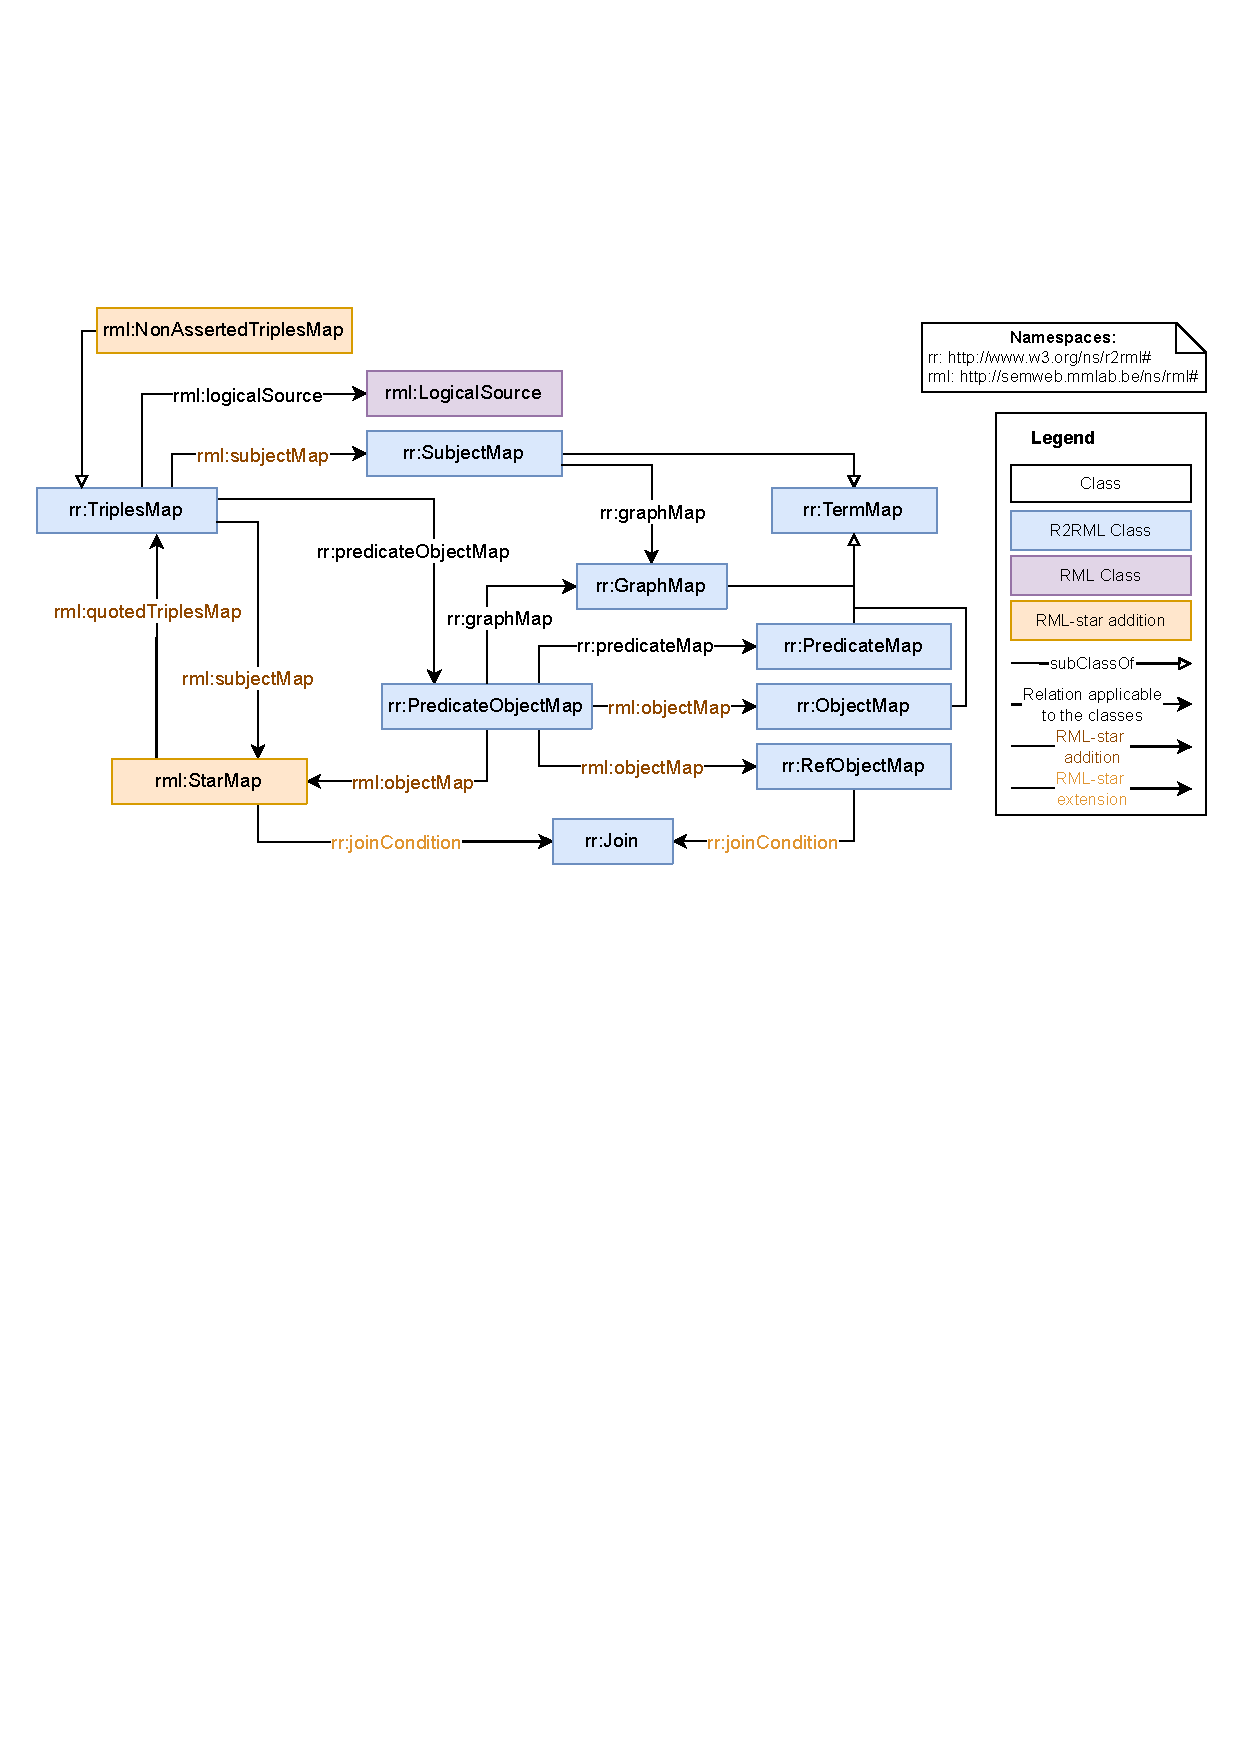
\includegraphics[width=1\linewidth]{figures/rml-star_diagram.pdf}
\caption{The \mbox{RML-star} extension (represented using the Chowlk notation~(\cite{feria2022chowlk})) with additions and modifications over the RML ontology.}
\label{fig:rml-star}
\end{figure*}

\begin{minipage}{\linewidth}
\centering
\begin{captionedlisting}{lst:chp4_rml-star}{Example RML-star mapping that transforms data in \cref{lst:chp4_csv_star}.}
\centering
\begin{multicols}{2}
{\begin{lstlisting}[numbers=left,basicstyle=\ttfamily\small,label={list:example1},columns=flexible,]
<#jumpTM> 
 a rml:NonAssertedTriplesMap ;
 rml:logicalSource :marks ;
 rml:subjectMap [ 
  rr:template ":{PERSON}" ] ;
 rr:predicateObjectMap [ 
  rr:predicate :jumps ;
  rml:objectMap [
   rml:reference "MARK" ] ] .
<#dateTM> 
 a rr:TriplesMap ;
 rml:logicalSource :marks ;
 rml:subjectMap [ 
  rml:quotedTriplesMap <#jumpTM>];
 rr:predicateObjectMap [ 
  rr:predicate :date ;
  rml:objectMap [
   rml:reference "DATE" ] ] .
\end{lstlisting}}

\end{multicols}
\end{captionedlisting}
\end{minipage}

\noindent\hspace{0.1\linewidth}\begin{minipage}{\linewidth}
\begin{captionedlisting}{lst:chp4_res-rml-star}{RDF-star triples generated by the mapping in \cref{lst:chp4_rml-star}.}
\centering
\begin{tabular}{c}
\hspace{2em}
{\begin{lstlisting}[basicstyle=\ttfamily\small,label={list:example1},columns=flexible]
<< :Angelica :jumps "4.80" >> :date "2022-03-21" .
<< :Katerina :jumps "4.85" >> :date "2022-03-19" .
\end{lstlisting}}
\end{tabular}
\end{captionedlisting}
\end{minipage}







\subsection{Validation}
\label{sec:chp4_validation}

We present the development of the RML star test-cases (\cref{sec:chp4_star_testcases}), that enables new implementations to check their conformance to RML-star; and create RML-star mappings for two real-world use cases (in \cref{sec:chp4_star_usecases}): software metadata extraction~(\cite{kelley2021framework} (SoMEF)) and biomedical research literature~(\cite{SemMedDB}) (SemMedDB). We use for both cases \mbox{Morph-KGC$^{star}$}, an implementation of RML-star.




\subsubsection{RML-star Test Cases}
\label{sec:chp4_star_testcases}

Test cases are commonly used %in standardization processes 
to evaluate the conformance of an engine with respect to a language specification (e.g., RML test cases~(\cite{heyvaert2019conformance})). 
A set of \mbox{RDF-star} test cases was proposed
covering the syntax of various of its serializations\footnote{\url{https://w3c.github.io/rdf-star/tests/}}.
We adapted these test cases to create the RML-star test cases and evaluate the conformance of \mbox{Morph-KGC$^{star}$}
with respect to \mbox{RML-star}.

To create a representative set of test cases for \mbox{RML-star}, we selected the N-Triples-star syntax tests\footnote{\url{https://w3c.github.io/rdf-star/tests/nt/syntax}}.  %;and follow a reverse engineering process. 
For each \mbox{RDF-star} test case, we created two associated \mbox{RML-star} test cases that generate the original \mbox{RDF-star} dataset: one test case with a single input data source (i.e., the mapping does not include joins) and another with two input data sources (i.e., the mapping includes joins among triple maps).
For each test case, we manually created the input source(s) in the CSV format and the corresponding \mbox{RML-star} mapping rules to generate the output \mbox{RDF-star} datasets.
Following this approach, we obtained 16 \mbox{RML-star} test cases.
The test cases are openly available at the W3C Community Group on Knowledge Graph Construction~(\footnote{\url{https://github.com/kg-construct/rml-star-test-cases}}),
and can be reused by any engine to test its conformance with respect to \mbox{RML-star}.


\subsubsection{Use Cases}
\label{sec:chp4_star_usecases}

We create RML-star mappings for in two real-world use cases. 
The first generates \mbox{RDF-star} graphs from scientific software documentation, 
and the second annotates statements extracted from biomedical research publications. 
For both use cases, we use the tool \mbox{Morph-KGC$^{star}$}.









%In order to ensure that these results in terms of time are representative, we run each mapping three times and calculate the average time.

%In both use cases we report the time on generating the RDF-star datasets. 




%In summary, our test and use cases show that \mbox{Morph-KGC$^{star}$} generates valid RDF triples and does not add an overhead in the generation time of reified triples. However, a more thorough analysis (out of the scope of this paper) is required to describe the behaviour of each mapping approach.

\noindent\textbf{\textit{Scientific Software Metadata Extraction.}}
Scientific software has become a crucial asset to deliver and reproduce the results described in research publications~(\cite{chue_hong_fair_2021}). However, scientific software is often time consuming to understand and reuse due to incomplete and heterogeneous documentation, available only in a human-readable manner.
The Software Metadata Extraction Framework (SoMEF)~(\cite{somef}) proposes an approach to automatically extract relevant metadata (description, installation instructions, citation, etc.) from code repositories and their documentation. SoMEF includes different text extraction techniques (e.g., supervised classification, regular expressions, etc.) that yield results with different confidence values.
For example, \cref{lst:JSONsnippet} shows a JSON snippet with the description that SoMEF obtained from a software repository (Widoco) using the GitHub API.
The confidence in this case is high as the extracted description was manually curated by the creators of the code repository.
SoMEF extracts more than 30 different metadata fields about 
software, its source code, its released versions, and their corresponding authors. For transforming the output of SoMEF into RDF-star, we used a total of 35 triples maps to annotate software metadata fields and an additional triples map to annotate source code descriptions. All reified triples follow the same structure (Listings \ref{lst:JSONsnippet} \& \ref{lst:TTLsnippet}), i.e. the standard RDF triple contains the excerpt of the extracted feature, and it is annotated
with the \emph{technique} used and the \emph{confidence} value. 
The complete mapping and all input examples and results are available online\footnote{\url{https://github.com/oeg-upm/rdf-star-generation}}.
 
\noindent\hspace{0.1\linewidth}\begin{minipage}{0.8\linewidth}
\begin{captionedlisting}{lst:JSONsnippet}{JSON snippet showing the description metadata field extracted by SoMEF on a code repository using the GitHub API as extraction technique.}
\centering
\hspace{3em}
{
\begin{lstlisting}[basicstyle=\ttfamily\small,label={list:example1},columns=flexible]
"codeRepository": "https://github.com/oeg-upm/Widoco",
"description": [ 
  {
    "confidence": [
      1.0
    ],
    "excerpt": "Wizard for documenting ontologies. WIDOCO is ...",
    "technique": "GitHub API"
  }
]  
\end{lstlisting}
}
\end{captionedlisting}
\end{minipage}

Capturing the technique used and the confidence obtained for each extracted metadata field is key for obtaining an accurate representation of the result. Hence, the \mbox{RDF-star} representation corresponding to the JSON in \cref{lst:JSONsnippet} includes this information, as depicted in \cref{lst:TTLsnippet}.

%\begin{minipage}{0.9\linewidth}
%\begin{captionedlisting}{lst:TTLsnippet}{N-Triples-star snippet showing the results generated for the %description field shown in \cref{lst:JSONsnippet}. Each asserted triple is annotated with its %corresponding confidence and technique.}
%\centering
%\begin{tabular}{c}
%\hspace{1.4em}
%{
%\begin{lstlisting}[numbers=left]
%<< <https://example.org/oeg-upm/Widoco> <https://w3id.org/okn/o/sd#description> 
%    "Wizard for documenting ontologies. WIDOCO is ..." >> 
%        <https://www.w3id.org/okn/o/em#technique> "GitHub API" .
%<< <https://example.org/oeg-upm/Widoco> <https://w3id.org/okn/o/sd#description> 
%    "Wizard for documenting ontologies. WIDOCO is ..." >> 
%        <https://www.w3id.org/okn/o/em#confidence> "1.0" .
%<https://example.org/oeg-upm/Widoco> <https://w3id.org/okn/o/sd#description> 
%    "Wizard for documenting ontologies. WIDOCO is ..." .
%\end{lstlisting}
%}
%\end{tabular}
%\end{captionedlisting}
%\end{minipage}        


\begin{captionedlisting}{lst:TTLsnippet}{RDF-star triples snippet showing the results generated for the description field in \cref{lst:JSONsnippet}. Each asserted triple is annotated with its corresponding confidence and technique.}
\centering
{
\begin{lstlisting}[basicstyle=\ttfamily\small,label={list:example1},columns=flexible]
ex:oeg-upm/Widoco :description "Wizard for documenting ontologies. WIDOCO is ..." .
<<ex:oeg-upm/Widoco :description "Wizard for documenting ontologies. WIDOCO is ...">> 
    :technique "GitHub API" .
<<ex:oeg-upm/Widoco :description "Wizard for documenting ontologies. WIDOCO is ...">> 
    :confidence "1.0" .
\end{lstlisting}
}
\end{captionedlisting}


%For example, for \cref{lst:JSONsnippet}, the excerpt of the software's description ("Wizard for documenting ontologies. WIDOCO is ...") was extracted with the technique "GitHub API" with a confidence of 1.0. 
% talk about the execution
%The reified triples are used for describing the software, that uses


\noindent\textbf{\textit{Biomedical Research Literature.}} 
SemMedDB~(\cite{SemMedDB}), the Semantic MEDLINE Database, is a repository 
that contains information on extracted biomedical entities 
and predications (subject-predicate-object triples) 
from biomedical texts (titles and abstracts from PubMed citations). 
%consists of a set of triples and annotations automatically extracted from PubMed titles, abstracts, and citations. 
%a set of data sources with automatic semantic annotations from titles and abstracts of citations available in PubMed.
The tables comprising SemMedDB are available for download as a relational database or CSV files\footnote{ \url{https://lhncbc.nlm.nih.gov/ii/tools/SemRep_SemMedDB_SKR/SemMedDB_download.html}}.
We downloaded the MySQL files for (1)~predication predictions (PREDICATION and PREDICATION\_AUX tables), containing more than 117 million annotations; and (2)~entity predictions (ENTITY table), which include more than 410 million annotations.
Listings \ref{lst:chp4_semmeddb_entity}, \ref{lst:chp4_semmeddb_pred} and \ref{lst:chp4_semmeddb_predaux} illustrate the columns used from the tables with synthetic data. 
For predications, only data for subjects is shown; the missing columns regarding objects follow the same structure as subjects.
%This data contains information on predicted entities and predicted subject-predicate-object predications.
Subjects and objects, from predications, and entities are assigned a semantic type 
(that categorizes the extracted concept in the biomedical domain) annotated with a confidence score. 
In addition, the extraction of subjects and objects is assigned a timestamp on when it took place. 
Thus, the score and timestamp represent metadata about other statements.
We created an RML-star mapping with 5 triples maps quoting triples:
3 of them are used to annotate the assignation of semantic types to entities, subjects, and objects with confidence scores;
the remaining 2 provide the timestamps for the extraction of subjects and objects. 

\begin{minipage}{0.38\linewidth}
\begin{captionedlisting}{lst:chp4_semmeddb_entity}{ENTITY table snippet.}
\centering
\begin{tabular}{c}
\hspace{-1em}
{
\begin{lstlisting}[basicstyle=\ttfamily\small,label={list:example1},columns=flexible]
ENTITY_ID , SEMTYPE , SCORE
12345     , orga    , 790
\end{lstlisting}
}
\end{tabular}
\end{captionedlisting}
\end{minipage}
\,\,\,\,\hfill
\begin{minipage}{0.6\linewidth}
\begin{captionedlisting}{lst:chp4_semmeddb_pred}{PREDICATION table snippet.}
\centering
\begin{tabular}{c}
\hspace{-1em}
{
\begin{lstlisting}[basicstyle=\ttfamily\small,label={list:example1},columns=flexible]
PREDICATION_ID , SUBJECT_SEMTYPE , SUBJECT_NAME
13579          , Semtype         , SubjName
\end{lstlisting}
}
\end{tabular}
\end{captionedlisting}
\end{minipage}

\noindent\hspace{0.23\linewidth}\begin{minipage}{0.8\linewidth}
\begin{captionedlisting}{lst:chp4_semmeddb_predaux}{PREDICATION\_AUX table snippet.}
\centering
\begin{tabular}{c}
\hspace{-7em}
{
\begin{lstlisting}[basicstyle=\ttfamily\small,label={list:example1},columns=flexible]
PREDICATION_AUX_ID, PREDICATION_ID, SUBJECT_SCORE, TIMESTAMP
67890             , 13579         , 800          , 1651740766
\end{lstlisting}
}
\end{tabular}
\end{captionedlisting}
\end{minipage}

\noindent\hspace{0.1\linewidth}\begin{minipage}{0.78\linewidth}
\begin{captionedlisting}{lst:chp4_semmeddb_triples}{RDF-star triples generated from data in Listings \ref{lst:chp4_semmeddb_entity}, \ref{lst:chp4_semmeddb_pred} and \ref{lst:chp4_semmeddb_predaux}.}
\centering
\begin{tabular}{c}
\hspace{-1.5em}
{
\begin{lstlisting}[basicstyle=\ttfamily\small,label={list:example1},columns=flexible]
<<ex:12345 sem:semanticType "orga">> sem:score "790" .
<<ex:13579 sem:subject ex:SubjName>> sem:timestamp "1651740766" .
<<ex:SubjName sem:semanticType "Semtype">> sem:score "800" .
\end{lstlisting}
}
\end{tabular}
\end{captionedlisting}
\end{minipage}


\section{Conclusions}

In this chapter, we performed an in-depth analysis of the features of the current mapping languages: from the description of input data sources, to how the triples are generated and data transformations. This analysis and the challenges proposed by the Knowledge Graph Construction W3C Community Group are gathered as requirements for a mapping language to be able to address the complexity of use cases for KG construction. Then, we presented the Conceptual Mapping, an ontology that, based on the abovementioned requirements, gathers the expressiveness of current mapping languages. This ontology was developed following the LOT methodology, and each step of the process and how if was addressed when building the ontology is explained. Finally, we show of mapping languages evolve as the semantic technologies advance, in this case with the adoption of RDF-star. To that purpose, we extend one of the most used mapping languages to create RDF-star graphs, RML-star. Accordingly, we add an extension to the Conceptual Mapping to include this new feature. Our ambition with this contribution is to enhance the understanding of the capabilities of mapping languages and what they need to implement in order to cover the necessities for constructing knowledge graphs, and at the same time be able to evolve as the technologies evolve.


\chapter{Enhancing the Creation of Mapping Rules}
\label{chapter:creation}

The mappings used for constructing knowledge graphs can be created in different ways. As they are formatted as text documents, they can be directly written in any text editor. However, the verbosity of some languages and the need of following a specific syntax has foster the development of user-friendly tools and serializations to ease the mapping writing process. This chapter introduces two solutions for easing the construction of mappings for different potential users, (i) a spreadsheet-based approach to write the mapping rules, and (ii) a user-friendly mapping syntax updated with the latest needs in knowledge graph construction.

\section{Mapping rules in spreadsheets: Mapeathor}
\label{sec:chp5_mapeathor}

Since mapping languages started to be used more broadly, there have been multiple approaches for the development of editors to ease their specification. Some of them enable editing through graphical visualization~\citep{heyvaert2016rmleditor,sicilia2017map}, while others provide a writing environment (e.g. the Protégé extension OntopPro~\ana{ref}). These editors are language-oriented, as they help to create mappings in a specific language. However, use cases require different features and implementations, and as a result, several different mapping languages are used currently. Moreover, graphical interfaces may hinder the mapping management and creation when a large number of mapping rules is required. 

%Moreover, when managing large amounts of mapping rules, graphical interfaces become cumbersome. %With our approach we aim at easing the writing process using a common tool such as spreadsheets, as well as enabling the generation of mapping files in more than one mapping language.

%In our work we focus on facilitating the transformation rule specification using declarative mapping rules. 
This section presents a straightforward approach to create these mapping documents, leveraging the  specification of mapping rules in spreadsheets. These spreadsheets contain the essential elements of the mapping rules without any additional syntax element, and are later translated into one a mapping document. The purpose of this proposal is to increase the interoperability between these languages~\citep{corcho2020towards, iglesias2022devising} as well as to ease the creation process. To perform the mapping rules translation we developed Mapeathor~\citep{iglesias-molina_2023_5973906}, a tool able to parse the spreadsheets and generate the corresponding mappings in R2RML, RML and YARRRML. Following, we present the structure of the spreadsheet to write the mapping rules, the implementation and a evaluation with a user study to validate our approach.

\subsection{Spreadsheet design}
\label{sec:chp5_spreadsheet_design}

%The rules required to generate a knowledge graph can be specified in multiple languages. The language is chosen by the user depending on the specific use case. However, the rules themselves are equivalent across languages, so they can be written in a language-independent way, in this case, we chose a spreadsheet for rule specification. 

In this section we present the design of the spreadsheet template to write the mapping rules. 
These mapping rules are specified in the spreadsheets following a provided structure to only write the essential information. Thus, this approach prevents the user from learning the syntax peculiarities of each languages (e.g. keywords, semicolons, brackets, etc.).
This design is devised to represent the rules in a compact and understandable manner, using a format widely used by the scientific community (i.e. Google spreadsheets, MS Excel). 
Using these spreadsheets along with their corresponding editors allow users to leverage their native advantages.

The mapping rules are specified in the spreadsheet across five different sheets, which are described below: \textit{Prefix sheet}, \textit{Source sheet}, \textit{Subject sheet}, \textit{Predicate\_Object sheet} and \textit{Function sheet}. We illustrate this section with a running example to describe in detail the expressiveness capabilities of each spreadsheet. This example uses the data represented in the CSV file \texttt{people.csv}(\cref{lst:chp5_mapeathor_input_people}) and the JSON file \texttt{sport.json} (\cref{lst:chp5_mapeathor_input_sport}). 

\begin{minipage}{0.48\linewidth}
\begin{captionedlisting}{lst:chp5_mapeathor_input_people}{ Contents of \texttt{people.csv}.}
\centering
\begin{tabular}{c}
%\hspace{1em}
{
\begin{lstlisting}[basicstyle=\ttfamily\small,label={list:example1},columns=flexible]
id , name  , birthdate , sport_id
1  , Emily , 08/02/90  , 2
2  , Jonah , 18/11/75  , 2
\end{lstlisting}
}
\end{tabular}
\end{captionedlisting}
\end{minipage}
\,\,\,\,\hfill
\begin{minipage}{0.52\linewidth}
\begin{captionedlisting}{lst:chp5_mapeathor_input_sport}{Contents of \texttt{sport.csv}.}
\centering
\begin{tabular}{c}
\hspace{1.5em}
{
\begin{lstlisting}[basicstyle=\ttfamily\small,label={list:example1},columns=flexible]
[ {
   "id": 1,
   "sport": " Ice Skating"
 },{
   "id": 2,
   "sport": " Rugby"
 } ]
\end{lstlisting}
}
\end{tabular}
\end{captionedlisting}
\end{minipage}


\subsubsection{Prefix sheet} 
This sheet contains the namespaces and corresponding prefixes used in the creation of the transformation rules. 
It is composed of two columns: \texttt{Prefix} for the prefix and \texttt{URI} for the corresponding namespace. The base namespace can be specified writing ``@base" in the \texttt{Prefix} column. The namespaces used by the target mapping language are automatically added in the translation (e.g. \texttt{rr}\footnote{\url{http://www.w3.org/ns/r2rml\#}}, \texttt{rml}\footnote{\url{http://semweb.mmlab.be/ns/rml\#}}).
The example shown in \cref{tab:chp5_prefix_sheet} presents how three namespaces and the base namespace are written in this template. 

\begin{table}[h!]
\caption{Prefix sheet.}
\label{tab:chp5_prefix_sheet}
\centering
\begin{tabular}{c|c}
\midrule
\textbf{Prefix} & \textbf{URI}                                 \\ \midrule
@base           & http://example.com/                          \\
rdf             & http://www.w3.org/1999/02/22-rdf-syntax-ns\# \\
ex              & http://ex.com/                               \\ 
grel            & http://semweb.datasciencelab.be/ns/grel\#     \\
\midrule
\end{tabular}
\end{table}


\subsubsection{Subject sheet} 
This sheet defines how to generate the subjects and a corresponding identifier (\texttt{ID}) that groups the mapping rules per subject. It is organized in four columns: \texttt{ID}, \texttt{URI}, \texttt{Class} and \texttt{Graph}. \texttt{ID} contains a unique identifier for each subject's set of rules in order to relate to information on these rules in the remaining sheets.
\texttt{URI} defines the subject URI of the resources that are to be generated by the mapping. 
\texttt{Class} allows the assignation of the subject to a class with \texttt{rdf:type}. A subject may be type of one class, more than one or none at all. 
Finally, \texttt{Graph} is an optional column that enables the assignation of a named graph to the triples generated for a subject.

The example shown in \cref{tab:chp5_subject_sheet} presents how to write two subjects, each with a different identifier and URI for the instances. Within the \texttt{URI} field, what is written between ``\{" and ``\}" references a field in the source data. The instances of the subject with the \texttt{PERSON} ID are type of two classes, (\texttt{ex:Person} and \texttt{ex:Athlete}), while all the triples of the instances of the subject identified with the \texttt{SPORT} ID are assigned to a named graph (\texttt{ex:SportsGraph}). 


\begin{table}[h!]
\caption{Subject sheet.}
\label{tab:chp5_subject_sheet}
\centering
\begin{tabular}{c|c|c|c}
\midrule
\textbf{ID} & \textbf{URI} & \textbf{Class} & \textbf{Graph} \\ \midrule
PERSON & http://ex.com/Person/\{name\} & ex:Person &  \\
PERSON & http://ex.com/Person/\{name\} & ex:Athlete &  \\
SPORT & http://ex.com/Sport/\{sport\} & ex:Sport & ex:SportsGraph \\ \midrule
\end{tabular}
\end{table}

\ana{no class}


\subsubsection{Source sheet} 

This sheet describes the source input data for each set of rules, identified with the identifier previously created in the \textit{Subject sheet} (\texttt{ID}). The information is organized in three columns: \texttt{ID}, \texttt{Feature} and \texttt{Value}. 
\texttt{ID} makes reference to the identifier that gathers the mapping rules in the sheets, which was introduced in the \textit{Subject sheet}. 
\texttt{Feature} declares the type of information provided in \texttt{Value}. The allowed keywords in this column are: \texttt{source} for the path and name of the file, \texttt{format} for the data source format, \texttt{iterator} for hierarchical data (e.g. JSON, XML), \texttt{table} for name of tables from Relational Data Bases (RDBs), \texttt{query} for SQL queries and \texttt{SQLVersion} for the version of SQL used. Each ID must have at least the \texttt{source} and \texttt{format} features specified, the rest of the features are optional. 
Then, in the \texttt{Value} column, the corresponding values of each \texttt{Feature} specified are written. 

\cref{tab:chp5_source_sheet} shows the data source description for the \texttt{PERSON} and \texttt{SPORT} IDs. The former corresponds to the CSV file shown in \cref{lst:chp5_mapeathor_input_people}, while the latter to the JSON file in \cref{lst:chp5_mapeathor_input_sport}, for which the iterator is also written (\texttt{\$.*}). 

\begin{table}[h!]
\caption{Source sheet.}
\label{tab:chp5_source_sheet}
\centering
\begin{tabular}{c|c|c}
\midrule
\textbf{ID} & \textbf{Feature} & \textbf{Value}              \\ \midrule
PERSON    & source          & /home/user/data/people.csv  \\
PERSON    & format          & CSV                         \\
SPORT     & source          & /home/user/data/sports.json \\
SPORT     & format          & JSON                        \\  
SPORT     & iterator        & \$.*                    \\ \midrule
\end{tabular}
\end{table}

\subsubsection{Predicate\_Object sheet} 
This sheet enable users to specify how to generate the triples, that is, predicate-object pairs for the subjects defined in the \textit{Subject sheet}. This sheet contains up to 8 columns: \texttt{ID}, \texttt{Predicate}, \texttt{Object}, \texttt{DataType}, \texttt{Language}, \texttt{ReferenceID}, \texttt{InnerRef} and \texttt{OuterRef}.

The column \texttt{ID} indicates the set of rules which the triples belong to, that has been previously defined in the \textit{Subject} and \textit{Source sheets}.
The columns \texttt{Predicate} and \texttt{Object} specify the predicate and object of the triple respectively. 
The XSD datatype of \texttt{Object} is defined in \texttt{DataType}, and the language tag in \texttt{Language}. Both these columns are optional. 

When the object refers to a subject defined in another mapping rule, the rule is written as follows. 
There are three columns that allow the specification of the linking condition between the object of the current triple and the referenced subject. 
They specify which is the ID of the referred subject  (\texttt{ReferenceID}), and the ``join'' fields in the source data: (i) \texttt{InnerRef} for the field of the object of the current triple, and (ii) \texttt{OuterRef} for the field of the referred subject. These three fields can be blank when a regular triple is produced. 

\cref{tab:chp5_po_sheet} shows five predicate-object pairs created for both sets of rules (\texttt{PERSON} and \texttt{SPORT}. Three of these rules produce literals with datatypes and two additionally specify a language tag. The rule set identified as \texttt{PERSON} generates a link to the subject of the \texttt{SPORT} rule set using the predicate \texttt{ex:name}, and joining by equal values of the field \texttt{sport\_id} from \texttt{people.csv} and the field \texttt{id} from \texttt{sport.json}. This rule set also calls a function for generating the object for the predicate \texttt{ex:birthdate}, which is identified by being enclosed by ``$<>$".

\begin{table}[h!]
\caption{Predicate\_Object sheet.}
\label{tab:chp5_po_sheet}
\centering
\resizebox{\columnwidth}{!}{
\begin{tabular}{c|c|c|c|c|c|c|c}
\midrule
\textbf{ID} &\textbf{Predicate} & \textbf{Object}               & \textbf{DataType} & \textbf{Language} & \textbf{ReferenceID} & \textbf{InnerRef} & \textbf{OuterRef} \\ \midrule
PERSON & ex:name & \{name\} & string & en & & &  \\
PERSON & ex:birthdate & $<$Fun-date$>$ & & & & & \\
PERSON & ex:plays & & & & SPORT& sport\_id & id \\
SPORT & ex:name & \{sport\} & string & en & & & \\
SPORT & ex:code & \{id\} & integer & & & & \\ \midrule
\end{tabular}
}
\end{table}

\subsubsection{Function sheet} Some languages are able to process data transformation functions, which can be detailed in this sheet. Mapeathor implements the last release of the RML-FNML specification, that describes how to incorporate functions in RML mappings\footnote{\url{https://w3id.org/rml/fnml/spec}}. The functions are referred in the \textit{Predicate\_Object sheet} or in other function rows with the identifier specified in \texttt{FunctionID}. The column \texttt{Feature} is used to specify the type of information provided in \texttt{Value}. The features admitted in the \texttt{Feature} column are \texttt{executes} for the name of the function, and \texttt{returns} for the expected output type of the function. In addition, this column admits any number of function parameter names. Then, the value of the name of the function, return type and values of the parameters are written correspondingly in the \texttt{Value} column.

The example shown in \cref{tab:chp5_function_sheet} uses the function \texttt{grel:toDate}, to change the formatting of a date. It returns a date as output (\texttt{grel:dateOut}) and takes three parameters: the data field to be converted (\texttt{grel:valueParam1}), the input data format (\texttt{grel:valueParam2}) and the output data format (\texttt{grel:valueParam3}).

\begin{table}[h!]
\caption{Function sheet.}
\label{tab:chp5_function_sheet}
\centering
\begin{tabular}{c|c|c}
\midrule
\textbf{FunctionID} & \textbf{Feature} & \textbf{Value} \\ \midrule
$<$Fun-date$>$ & executes & grel:toDate \\  
$<$Fun-date$>$ & returns & grel:dateOut \\  
$<$Fun-date$>$ & grel:valueParam1 & \{birthdate\} \\
$<$Fun-date$>$ & grel:valueParam2 & dd/MM/yyyy \\
$<$Fun-date$>$ & grel:valueParam3 & yyyy-MM-dd \\
\midrule
\end{tabular}
\end{table}


\subsection{Mapeathor}
\label{sec:chp5_mapeathor_tool}

Mapeathor~\citep{iglesias-molina_2023_5973906} is a open-source implementation to generate mappings from the spreadsheets described in \cref{sec:chp5_spreadsheet_design}. It is able to process MS Excel and Google Spreadsheets, generating human-readable mappings in either R2RML, RML or YARRRML. 

\cref{alg:mapeathor} presents the procedure implemented by Mapeathor to translate an input spreadsheet into a formatted mapping document. First, the rules written in the spreadsheet template are extracted and stored in a JSON file. This step also validates that the spreadsheet follows correctly the template. The prefixes are then added to the output mapping document, along with other prefixes that are used nativetly in the target language (e.g. \texttt{r2rml}, \texttt{rml} \ana{prefijo rml}). Then, the rules are translated by grouping them into rulesets with the same \texttt{ID} expressed in the spreadsheet (see \ana{previous section with template and subject)}. The extracted rules are enriched with implicit information needed to write the mapping (e.g. to look for \textit{rr:TermTypes} and IRIs). Next, the subject, source and predicate-object pairs in each ruleset are translated. In the case of RML, the system also looks for referencing functions to translate them as well. Finally, the translated rules are written into a final file, which is returned as output. The mapping documents are written by the system in a human-readable manner. \ana{ojo que esto se parece a yatter } \ana{listing whatever } shows the output RML mapping that Mapeathor produces after processing the rules written in the spreadsheet shown in Tables \ref{tab:chp5_prefix_sheet}, \ref{tab:chp5_subject_sheet}, \ref{tab:chp5_source_sheet}, \ref{tab:chp5_po_sheet} and \ref{tab:chp5_function_sheet}. 


The source code of Mapeathor is openly available under Apache 2.0 license\footnote{\url{https://github.com/oeg-upm/mapeathor}}. It can be run as a CLI using the Pypi package\footnote{\url{https://pypi.org/project/mapeathor/}} or as an online service\footnote{\url{https://morph.oeg.fi.upm.es/demo/mapeathor}}, where a visual interface is provided. With each release, a new version in Pypi is created and a dedicated DOI archived in Zenodo~\citep{iglesias-molina_2023_5973906}. 


\begin{minipage}{0.95\linewidth}
\begin{algorithm}[H]
\SetAlgoLined
\KwResult{Mapping document in [R2]RML/YARRRML}
 $language \longleftarrow output\_language$\;
 $spreadsheet \longleftarrow input\_spreadsheet$\;
 $output\_m \longleftarrow \emptyset$\;
 $rules \longleftarrow extract\_rules(spreadsheet)$\;
 $output\_m.add(translate\_prefixes(rules))$\;
  
 \For{$ruleset \in rules$}{
    $rules.add(enrich\_ruleset(ruleset))$\;
    $output\_m.add(translate\_subject, language)$\;
    $output\_m.add(translate\_source, language)$\;
    $output\_m.add(translate\_predicate\_object, language)$\;
    \If{$language == RML$}{
        $output\_m.add(translate\_functions)$\;
        }
    }
 
 \Return{$validate(write\_m)$}\;
\caption{Mapeathor translation algorithm}
\label{alg:mapeathor}
\end{algorithm}
\end{minipage}

\begin{captionedlisting}{lst:chp5-1_rml-output}{RML mapping generated with Mapeathor with the spreadsheet shown in Tables \ref{tab:chp5_prefix_sheet}, \ref{tab:chp5_subject_sheet}, \ref{tab:chp5_source_sheet}, \ref{tab:chp5_po_sheet} and \ref{tab:chp5_function_sheet}. }
\centering
{\begin{lstlisting}[numbers=left,basicstyle=\ttfamily\small,columns=flexible]
@prefix rr: <http://www.w3.org/ns/r2rml#>.
@prefix xsd: <http://www.w3.org/2001/XMLSchema#>.
@prefix rml: <http://semweb.mmlab.be/ns/rml#>.
@prefix ql: <http://semweb.mmlab.be/ns/ql#>.
@prefix rdf: <http://www.w3.org/1999/02/22-rdf-syntax-ns#>.
@prefix ex: <http://ex.com/>.
@prefix grel: <http://semweb.datasciencelab.be/ns/grel#>.
@base <http://example.com/>.

<#PERSON>
    a rr:TriplesMap;
    rml:logicalSource [
    	rml:source "/home/user/data/people.csv";
    	rml:referenceFormulation ql:CSV;
    ];
    rr:subjectMap [
    	a rr:Subject ;
    	rr:termType rr:IRI ;
    	rr:template "http://ex.com/Person/{name}" ;
    	rr:class ex:Person ;
    	rr:class ex:Athlete ;
    ];
    rr:predicateObjectMap [
    	rr:predicateMap	[ rr:constant ex:name];
    	rr:objectMap	[ rml:reference "name"; 
                      rr:termType rr:Literal;  
                      rr:datatype xsd:string;  
                      rr:language "en" ]
    ];
    rr:predicateObjectMap [
    	rr:predicateMap	[ rr:constant ex:plays ];
    	rr:objectMap	[
    		rr:parentTriplesMap	<#SPORT>;
    		rr:joinCondition	[
    			rr:child	"sport_id";
    			rr:parent	"id";
    		];
    	];
    ];
    rr:predicateObjectMap [
      rr:predicateMap	[ rr:constant ex:birthdate] ;
      rr:objectMap	[
    	  rml:functionExecution <#Fun-date> ;
    	  rml:return grel:dateOut ;
    	];
    ]; .

<#SPORT>
    a rr:TriplesMap;
    rml:logicalSource [
    	rml:source "/home/user/data/sports.json";
    	rml:referenceFormulation ql:JSONPath;
        rml:iterator "$\dollar$.*";
    ];
    rr:subjectMap [
    	a rr:Subject ;
    	rr:termType rr:IRI ;
    	rr:template "http://ex.com/Sport/{sport}" ;
    	rr:class ex:Sport ;
    	rr:graphMap [ rr:constant "ex:SportsGraph" ] ;
    ];
    rr:predicateObjectMap [
    	rr:predicateMap	[ rr:constant ex:name];
    	rr:objectMap	[ rml:reference "sport";  
                      rr:termType rr:Literal;  
                      rr:datatype xsd:string;  
                      rr:language "en" ]
    ];
    rr:predicateObjectMap [
    	rr:predicateMap	[ rr:constant ex:code];
    	rr:objectMap	[ rml:reference "id";  
                      rr:termType rr:Literal;  
                      rr:datatype xsd:integer ]
    ]; .

<#Fun-date> a rml:FunctionExecution;
    rml:function grel:toDate ;
    rml:input [
      a rml:Input ;
      rml:parameter grel:valueParam1 ;
      rml:inputValueMap [ rml:reference "birthdate" ];
    ];
    rml:input [
      a rml:Input ;
      rml:parameter grel:valueParam2 ;
      rml:inputValueMap [ rr:constant "dd/MM/yyyy" ];
    ];
    rml:input [
      a rml:Input ;
      rml:parameter grel:valueParam3 ;
      rml:inputValueMap [ rr:constant "yyyy-MM-dd" ];
    ]; .
\end{lstlisting}}
\end{captionedlisting}

\subsection{Evaluation}
We evaluate the presented approach by performing a user study with two dimensions to test the usability of Mapeathor and check if the spreadsheet-based approach can improve the mapping writing process for users of different expertise. 

\begin{table}[t!]
\caption{Questionnaire for subjective assessment of the usability of the spreadsheet design and Mapeathor. }
\centering
\label{tab:chp5_sub_questionnaire}
\resizebox{\columnwidth}{!}
{\begin{tabular}{cl}
\multicolumn{2}{c}{\textbf{Questions}} \\ \midrule
1. & I think that I would like to use this tool frequently\\ \midrule
2. & I found the tool unnecessarily complex\\ \midrule
3. & I thought the spreadsheet template was easy to use\\ \midrule
4. & I think that I would need the support of a technical person to be able to use the spreadsheet template\\ \midrule
5. & I found the different facets in this spreadsheet template were well integrated\\ \midrule
6. & I thought there was too much inconsistency in this tool\\ \midrule
7. & I think that most people would learn how to write the spreadsheet template very quickly\\ \midrule
8. & I found the tool unmanageable to use\\ \midrule
9. & I felt very confident using the spreadsheet template\\ \midrule
10. & I needed to learn a lot of things before I could get going with this tool\\ \midrule
11. & Optional comments (feedback to improve) \\ \bottomrule
\end{tabular}}
\end{table}

\subsubsection{Methodology}
\label{sec:chp5_mapeathor_eval_method}

The evaluation is performed in two steps. We first carry out a \textit{subjective evaluation} in order to gather opinions and feedback about the spreadsheet template and usability of the tool in order to improve the user experience. We then perform a \textit{objective evaluation} to find out if our approach improves the mapping writing process w.r.t. writing directly the mapping in a target language (i.e. RML) and w.r.t. another mapping editor with a visual interface (i.e. RMLEditor). This section describes the methodology followed for the performed evaluations.

%\textit{motivación: qué queremos comprobar, que si facilita la creación de mapping rules para experts y no experts. Para eso llevamos a cabo dos evaluaciones con usuarios, subjectiva y objetiva. En la subjectiva usuarios que han probado el software cuentan su experiencia y opiniones. En la objetiva, cogemos a usuarios y los dividimos en 3 grupos, para que generen mappings con rml, rmleditor y mapeathor. Así vemos si 1) mapeathor mejora RML y si 2) funciona mejor que una herramienta visual. Describir background, que no hay bias porque se puso a gente que nos había utilizado esa tech antes. y resultados}


\noindent\textit{\textbf{Procedure}} The evaluation is comprised of two steps. The first step, correspondent to the \textit{subjective evaluation}, took place during the Knowledge Graph Construction Tutorial co-located with the 19th edition of the Extended Semantic Web Conference (2022)\footnote{\url{https://kg-construct.github.io/eswc-dkg-tutorial-2022/}}. This tutorial hosted a slot for presenting Mapeathor and the spreadsheet design, allowing time for a hands-on exercise at the end of the explanation. At the end of the slot, participants were asked to fill a questionnaire to assess the usability of the approach and gather some feedback for improvements. The questionnaire first inquired about the background of the participants, asking them to rate in a 5-point Likert scale their expertise in (i) linked data and (ii) mapping languages and tools. Then, it assessed the usability of the approach with 10 questions that follow the SUS template, with also a 5-point Likert scale rating; and an additional optional question to gather feedback for improvement (\cref{tab:chp5_sub_questionnaire}).








The second step of the evaluation that comprises the \textit{objective evaluation} took place in May 2023, once the improvements gathered from the previous step were implemented. In this step, the spreadsheet-based approach proposed in this work was compared with the widely used RML mapping language~\citep{Dimou2014rml}, and with a visual editor, RMLEditor~\citep{heyvaert2016rmleditor}. A group of 30 participants was divided into three groups of 10. Each group had to carry out the same task, to create a mapping from a given dataset and ontology with the assigned tool. All groups were introduced to the needed concepts about mapping languages and specific guidelines with examples of the assigned tool. The groups performed the given task in separated sessions, i.e. one session per tool was carried out, to ensure that all participants were given the same level of assistance independently of the tool. Participants were asked to carry out the proposed task in 30 minutes. Having reached the time limit, they were asked to submit the mapping they have created so far. In addition, in the same way as in the first step, participants were asked to rate in a 5-point Likert scale their expertise in (i) linked data and (ii) mapping languages and tools; and to write their personal opinion on the assigned tool.


\begin{figure*}[!t]
\centering
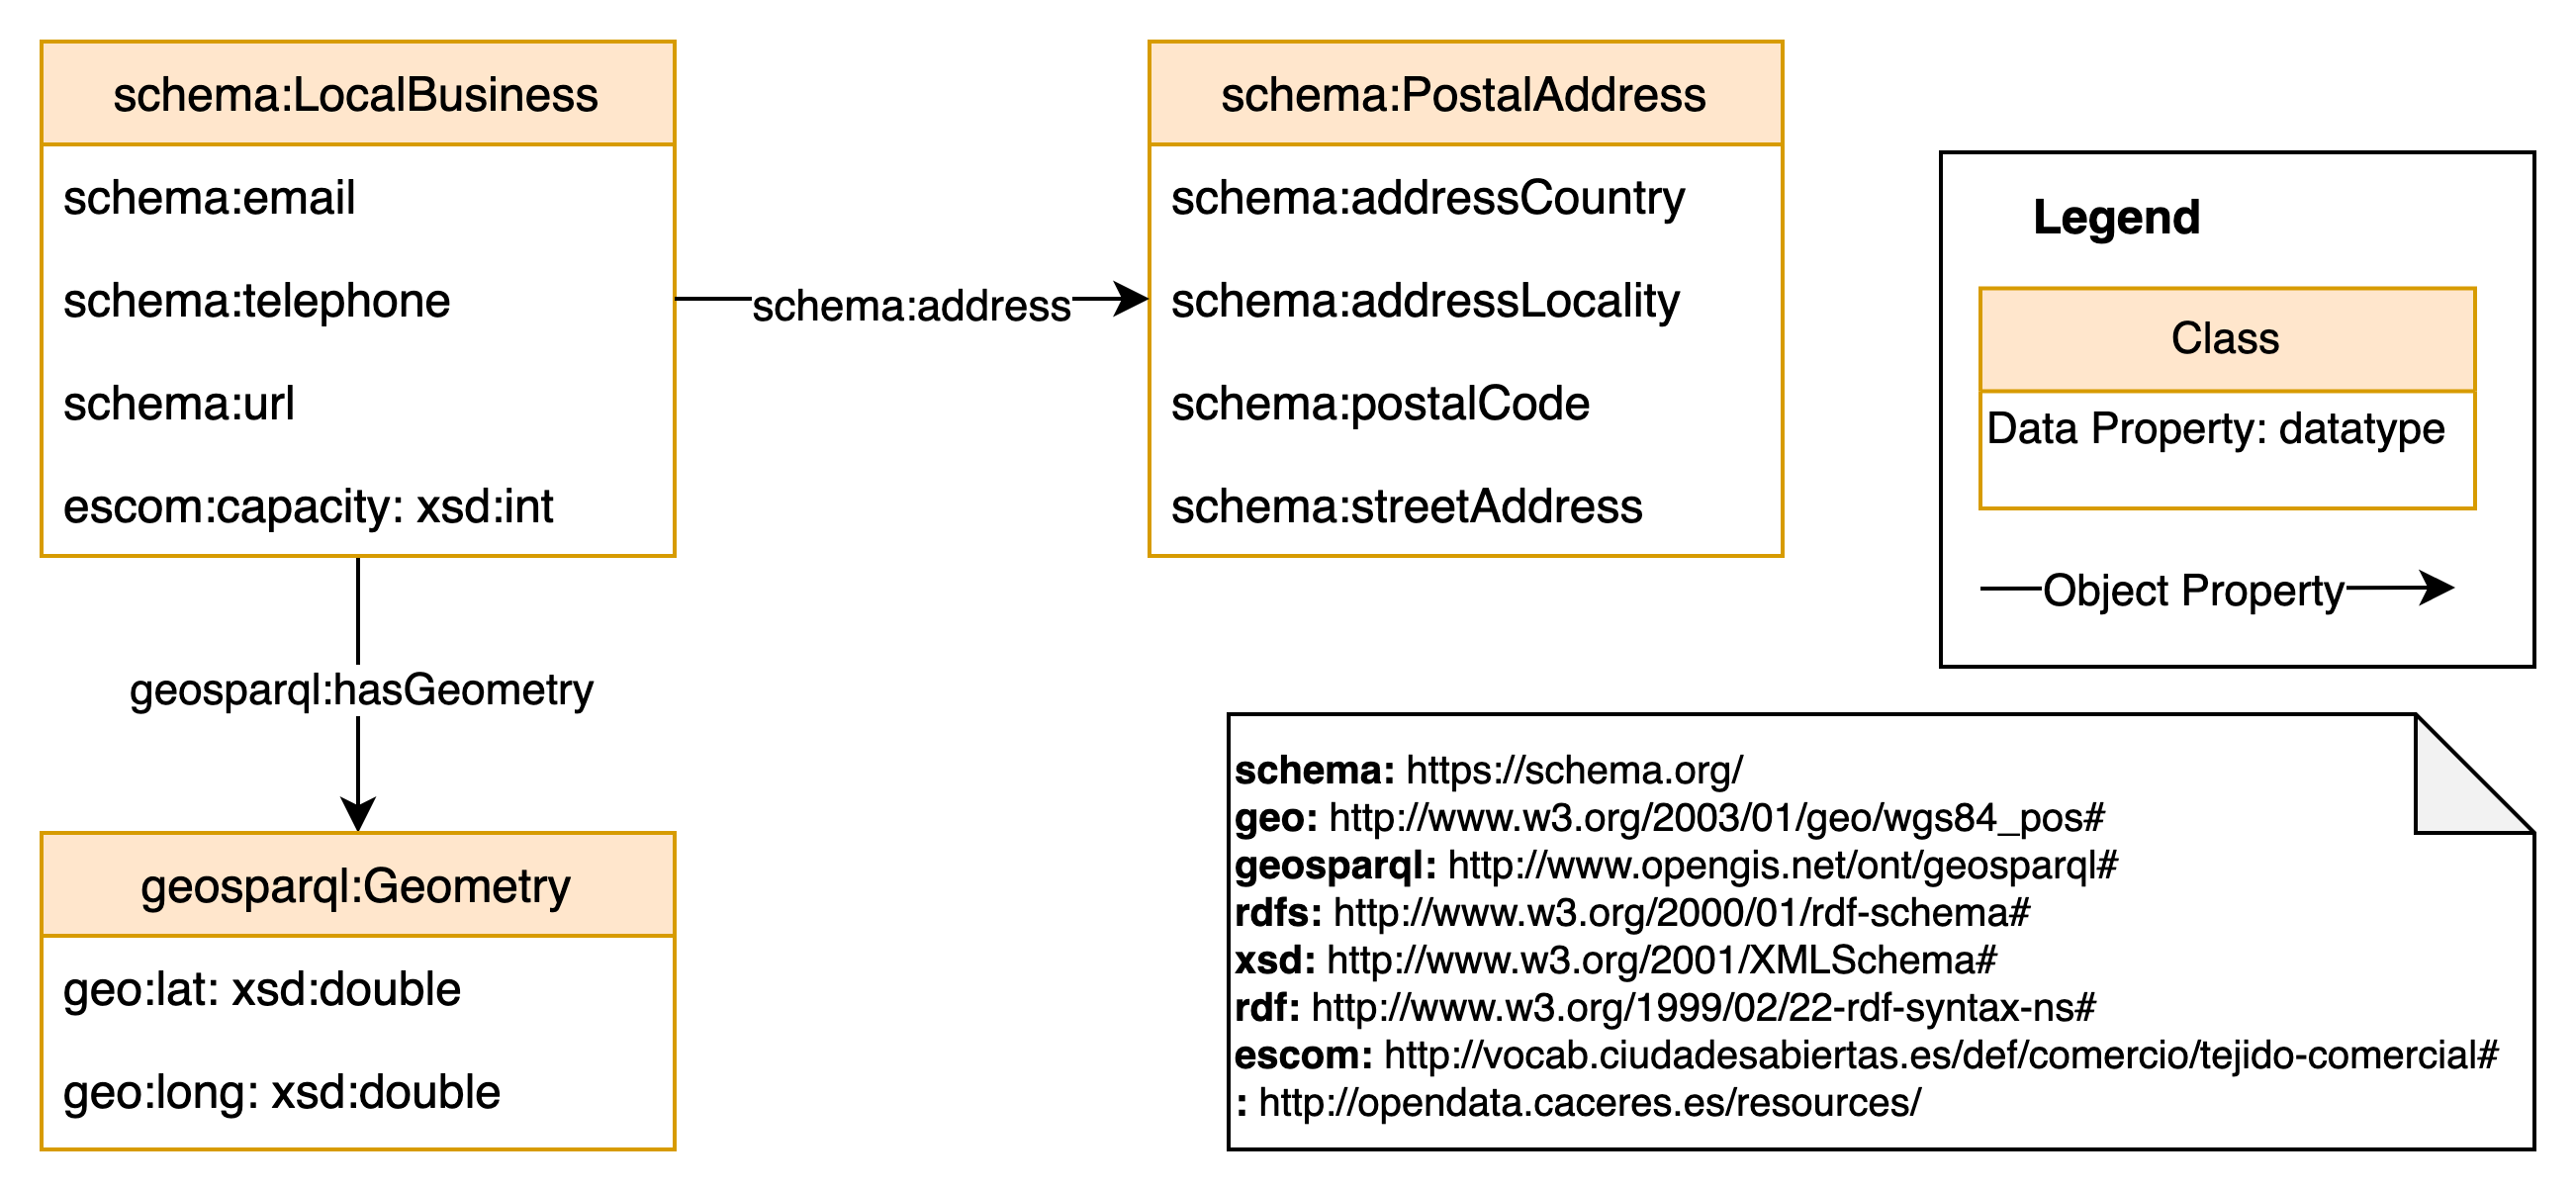
\includegraphics[width=\linewidth]{figures/chp5-1_us_onto.png}
\caption[Ontology diagram for the user study exercise of Mapeathor]{Ontology diagram representing a subset of the Vocabulary for data representation of the local business census and activities licenses.}
\label{fig:chp5-1_us_onto}
\end{figure*}

\noindent\textit{\textbf{Resources}}
The same data and ontology was used for both evaluations. We use a subset of the \textit{Vocabulary for data representation of the local business census and activities licenses}\footnote{\url{http://vocab.ciudadesabiertas.es/def/comercio/tejido-comercial/index-en.html}} that represents local businesses, their postal address and geolocalization (\cref{fig:chp5-1_us_onto}). 
We chose this dataset, that belongs to the common-knowledge domain, to avoid heterogeneous prior domain knowledge influence on the results of the study.

We provided participants with the subset ontology description and associated data, that is comprised of three CSV files: \texttt{bar.csv}, \texttt{restaurant.csv} and \texttt{address.csv}. Information about bars, restaurants and their geolocalization is represented in the files \texttt{bar.csv}, \texttt{restaurant.csv} respectively. 
These files contain the same columns, but different data. The file \texttt{address.csv} represent the postal address of the businesses present in the other two files. 
The original data is available in GitHub\footnote{\url{https://github.com/CiudadesAbiertas/vocab-comercio-censo-locales/}}. 
To facilitate the exercise for participants, some data cleaning was performed over the original files, as well as translation to all columns form spanish to english. The used resources are published in Zenodo~\citep{iglesias-molina_2022_8154522}.



\noindent\textit{\textbf{Participants}} 
In the \textit{subjective evaluation}, 17 attendants submitted answers to the questionnaire provided during the session. Most of the participants were knowledgeable in linked data, while less than half had already used mappings before. 
In the \textit{objective evaluation}, 30 participants were sampled from the Ontology Engineering Group, ranging from MSc students to full professors. Their background ranged from having basic knowledge about linked data and mappings, to being knowledgeable practitioners, including participants that were experts in linked data but had no knowledge about mappings. Prior to the assignation of participants to each group, participants were asked to provide information about whether they had prior knowledge of any of the tools, so that no participant would use a tool which they were already familiar with. Taking into account this restriction, they were randomly divided into three groups, one per tool. Each group was balanced w.r.t. the heterogeneity in background (\cref{fig:chp5-1_expertise}). 


\begin{figure*}[!t]
\centering
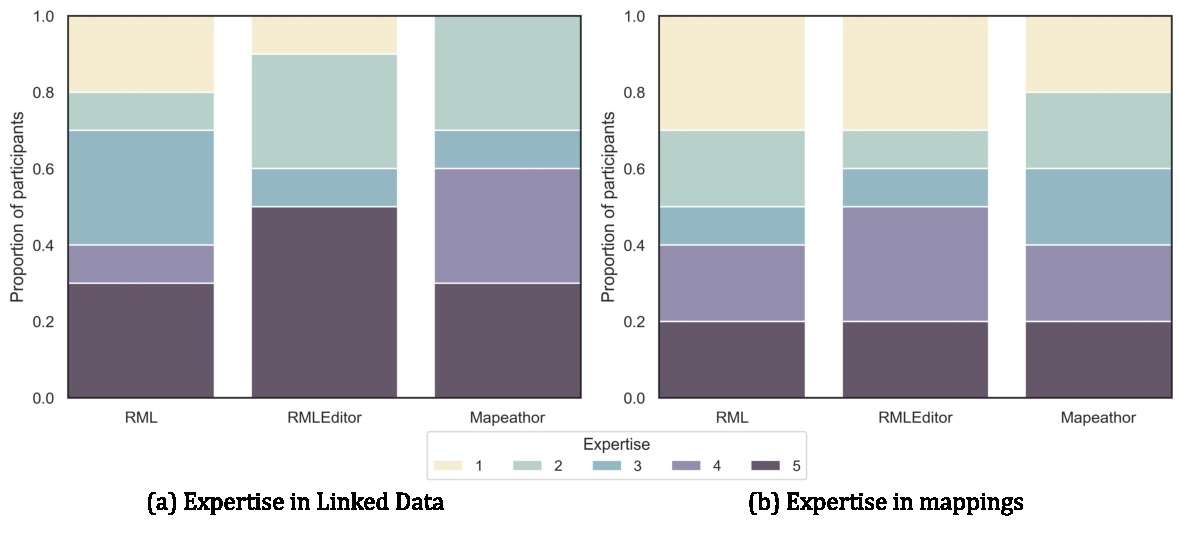
\includegraphics[width=1\linewidth]{figures/chp5-1_expertise.pdf}
\caption[Expertise of participants of the user study.]{Distribution of expertise of participants according to the 5-point Likert scale in (a) Linked Data and (b) mappings.}
\label{fig:chp5-1_expertise}
\end{figure*}

\noindent\textit{\textbf{Metrics}} 
The \textit{subjective evaluation} measured the responses to the SUS questionnaire on a 5-point Likert scale. 
For the \textit{objective evaluation},
%the accuracy of the mapping submitted was calculated. All participants had 30 minutes to perform the task and upload the resulting mapping, thus two kinds of accuracies are calculated. \ana{igual esta frase cuadrarla después }
we calculate two kinds of accuracies: (i)~\textit{Total Accuracy} (TA) for the number of correct rules written w.r.t. the reference correct mapping, and (ii)~\textit{Local Accuracy} (LA) for the number of correct rules w.r.t. all the written rules. We calculate both accuracies because of the fixed time for completing the exercise. TA can be interpreted as a measure of completeness, while LA focusses on assessing the correctness of the written rules independently on the total completeness.
We divide the mapping in four components: \textit{Subject}, \textit{Source}, \textit{Predicate-Object (PO)} and \textit{Join}, and calculate the accuracy for each component and the totality of the mapping. Then a T-Test is performed to look for significant differences of accuracy among the tools. This test is sed under the assumptions of (i) normality, (ii) sameness of variance, (iii) data independence, and (iv) variable continuity.


\noindent\textit{\textbf{Threats to validity}}~\citep{creswell2017research} We identify the following internal and external threats to the validity of our experiment.

\textbf{Internal validity threats} concern the experimental setup or experience of participants which threaten the ability to draw correct conclusions about the population in the experiment. We identify three internal threats: \textit{tool familiarity bias}, \textit{selection bias} and \textit{instruction bias}.
\begin{itemize}
    \item \textbf{Tool familiarity bias.} Practitioners tend to be more expert in some specific technologies and languages that they use more frequently. Thus, in the sample there it is possible to have participants that have used any of the tested approaches, which in turn can influence the results. For creating the groups, participants' experience was inquired to avoid assigning them a tool that they had previously used.
    \item \textbf{Selection bias.} The sample includes participants with different range of skills and previous knowledge about linked data and mappings. We mitigate this threat by defining groups that were  homogeneous w.r.t. range of expertise in mappings and linked data, considering also the mitigation measures for the \textit{tool familiarity} threat. That is to say, all groups included from beginner users to knowledgeable practitioners. 
    \item \textbf{Instruction bias.} One of the evaluated approaches is designed by the conductors of the user study. This situation could incur in bias on information delivery. To mitigate this threat, we provided participants with the same instruction guidelines for each tool. Three sessions were conducted subsequently to provide the same explanations and attention to each tool. During each sessions, all questions were answered with equal level of detail and guidance for all tools and participants.
\end{itemize}

\textbf{External validity threats} occur when wrong inferences from sample data are made beyond the studied sample or experimental setup. We identify two external threats: \textit{background of participants sample} and \textit{environment}.
\begin{itemize}
    \item \textbf{Background of participants sample.} This threat concerns the generalization to individuals outside the study. The sample of participants include a wide range in the variety of backgrounds, from not very familiar with linked data and mappings, to expert practitioners. We deliberately choose to have this variety for each group so that the results can be generalized to a broader sample, while mitigating the risks of internal threats described above that this choice poses. 
    \item \textbf{Environment.} This threat concerns the generalization to individuals outside the experiment’s setting. Participants were free to use a computer, browser and tools of their choice. Thus, they could perform the tasks required for the study in a well-known environment. No specific experimental setup prevents generalizations to individuals outside our study.
\end{itemize}




\subsubsection{Results}
\label{sec:chp5_mapeathor_results}

\noindent\textit{\textbf{Subjective evaluation results}}


\begin{table}[!t]
\caption{Results of the user study, showing the mean of the local accuracy (LA), total accuracy (TA) and p-value of the submitted responses per mapping feature and tool. }
\label{tab:chp5-1_summary_results}
\centering
\resizebox{\columnwidth}{!}
{\begin{tabular}{ccc|cc|cc|cc|cc}
    \cmidrule{2-11}
    & \multicolumn{2}{c|}{\textbf{Subject}} & \multicolumn{2}{c|}{\textbf{Source}} & \multicolumn{2}{c|}{\textbf{PO}} & \multicolumn{2}{c|}{\textbf{Join}} & \multicolumn{2}{c}{\textbf{Total}} \\ \cmidrule{2-11}
    & LA & TA & LA & TA & LA & TA & LA & TA & LA & TA \\ \midrule
    \textbf{\makecell{RML}} & 0.617 & 0.457 & 0.927 & 0.570 & \underline{0.684} & 0.458 & \underline{0.133} & \underline{0.150} & \underline{0.693} & 0.410  \\ \midrule
    \textbf{\makecell{RMLEditor}} & \underline{0.465} & \underline{0.360} & \underline{0.860} & \underline{0.560} & 0.705 & \underline{0.363} & 0.233 & 0.217 & 0.705 & \underline{0.340}  \\ \midrule
    \textbf{Mapeathor} & \textbf{0.858} & \textbf{0.620} & \textbf{0.960} & \textbf{0.620} & \textbf{0.795} & \textbf{0.581} & \textbf{0.250} & \textbf{0.225} & \textbf{0.831} & \textbf{0.547}  \\\midrule \midrule
    \textbf{p-value} & 0.090 & 0.295 & 0.596 & 0.890 & 0.777 & 0.337 & 0.746 & 0.881 & 0.476 &  0.264 \\ \bottomrule
\end{tabular}}
\end{table}

\noindent\textit{\textbf{Objective evaluation results}}

%\ana{e ir intercalando opiniones sobre cada approach para apoyar los resultados, ambas buenas y malas}
%\ana{de rmleditor fallos a nivel técnicos, opiniones divididas entre intuitivo/antiintuitivo, hay constructos que hay que explicar, pero una vez superada esa barrera medianamente bien. Remarcan que faltan funcionalidades como copy/paste de secciones enteras, y buscar mejor lo creado en el espacio de trabajo (a muchos se les perdían las cosas y había que volver a empezar)}
%\ana{de rml igual hay mejores resultados porque una vez se entienden las partes del mapping y partiendo de un ejemplo, qué hay que copiar y cambiar, eso agiliza el proceso. Más indicado para desarrolladores (más acostumbrados a escribir código), se señala que no es excesivamente complejo pero con alguna herramienta se haría mejor.}
%\ana{curva de aprendizaje de la herramienta, como todos, pero en general gusta que se pueda usar algo tan común como excel, que facilita mucho la escritura de reglas. El punto negativo viene por el tema de los IDs, que al no aparecer automáticos en las subsecuentes pestañas induce a errores.}

%% In general
\cref{tab:chp5-1_summary_results} shows the results obtained from the user study. In general, it can be observed that Mapeathor obtains the highest accuracy rate in all cases. Surprisingly, RMLEditor struggles with the base approach, RML, obtaining in general slightly worse results. Between these two approaches, participants using RML were able to complete more total mapping rules, while for RMLEditor the written rules were more accurate. 

%% no significance, but tendencies in differences in parts
However, none of the differences in the results for any type of mapping rule is significant (p-values $>$ 0.05), but we can observe some tendencies. The results for which the p-value is closer to being significant is for the total accuracy of the complete mapping, and for the subjects (specially its local accuracy). In this cases, it can be stated with more confidence that Mapeathor can help the writin process. 
%\textit{sin embargo, ninguno de los resultados es significativo (p-value $<$ 0.05), pero sí se pueden observar tendencias. Los resultados donde más se acerca el p-value a ser significativo es para el total accuracy del mapping completo, y para la escritura de los sujetos, especialmente en el local accuracy. En estos casos se puede afirmar con más seguridad que Mapeathor va bien encaminado a mejorar la escritura de las mapping rules.}  \ana{de donde rmleditor supera a rml tb?}

%% analysis of parts of mappings
Looking at the details of each mapping parts, in general the writing of \textit{Sources}, \textit{Subjects} and \textit{Predicate-Object} pairs (\textit{PO}) is carried out mostly successfully. It is especially remarkable for \textit{Sources}, that achieves a local accuracy near to 1. However, the results reported for its total accuracy are not that high, which can be due to the time limit and the increasing complexity of the exercise. The accuracy of the creation of \textit{Subjects} with the RMLEditor is rather low w.r.t the other approaches. \ana{detalle de los fallos comunes para este caso, mirar mappings directamente}. The mapping element where all approaches fail to assist users is unmistakably the \textit{Joins}. Most participants did not even try to write them, and those who did mostly failed. 

%\textit{mirando más en detalle a cada una de las partes del mapping, se puede ver que en general la escritura de sujetos, sources y poms es muy exitosa, sobre todo de los sources, donde el local accuracy de todos los approaches es cercanoa 1. regarding el total accuracy, los resultados no son tan buenos, en parte puede ser por el tiempo dado, y en parte por la complejidad incremental del mapping. que había dos sujetos creados a partir del mismo archivo, y dos archivos que servian para crear el mismo sujeto. Donde todas las herramientas fallan estrepitosamente es en la creación de joins, llevandose la palma RML. Aquí si se puede ver que los user-friendly approaches si apoyan a la escritura, pero sin mucho éxito tampoco.}


%% en general



\begin{figure}[t!]
    \centering
    \begin{subfigure}[b]{\linewidth}
    	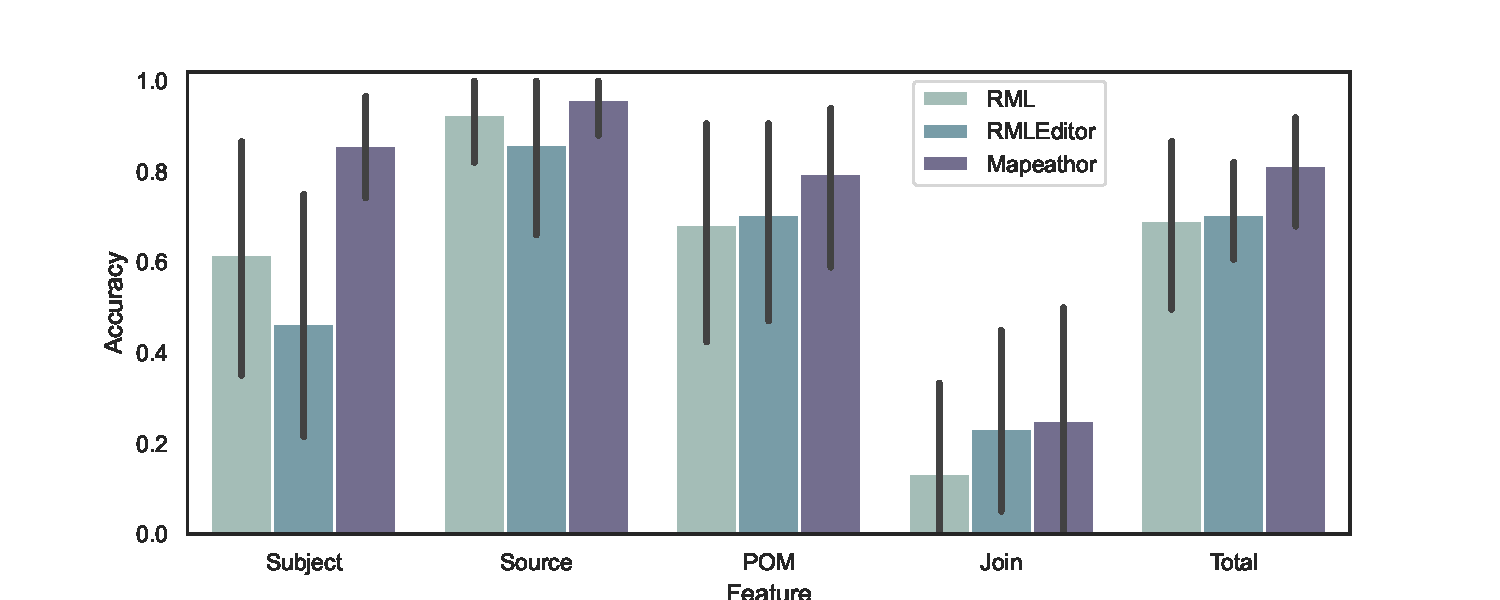
\includegraphics[width=\linewidth]{figures/mapeathor_rel-acc.pdf}
    	\caption{Local accuracy.}
    	\label{fig:chp5_mapeathor_relacc}
    \end{subfigure}
   %\hspace{0.05\textwidth}
    \begin{subfigure}[b]{\linewidth}
    	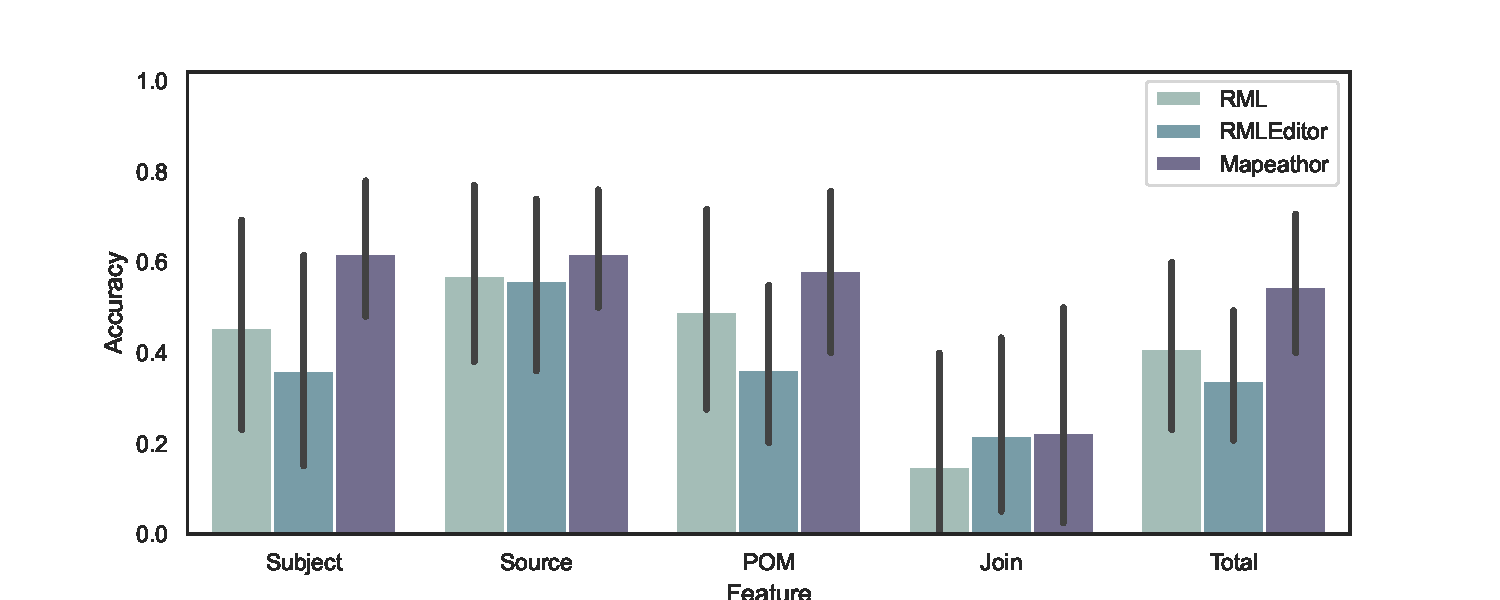
\includegraphics[width=\linewidth]{figures/mapeathor_total-acc.pdf}
    	\caption{Total accuracy.}
    	\label{fig:chp5_mapeathor_totacc}
    \end{subfigure}
    \caption{Accuracy results.\ana{estando la tabla esto queda redundante?}}
    \label{fig:reification-app}
\end{figure}


%\subsection{Use cases}
%Ciudades abiertas, EBOCA, photocatalisis ontology
%\ana{bueno ya veremos}



\subsection{Discussion}
\label{sec:chp5_mapeathor_discussion}
\ana{discusión de resultados, y use cases también se pueden comentar. O al igual si no es mucho se puede decir directamente en las conclusiones del capítulo}

In general, the results obtained in the user study show that there is still plenty of room for improvement for facilitating the adoption and use of mappings by a broader community of users. In each group, there were participants able to completely finish the exercise on time. In addition, plenty other participants claimed (in the feedback space left in the questionnaire) that, without the time limit, it would have been possible for them to complete the mappings. However, the reported local accuracy indicates that, even complete, the mapping would not have been entirely valid. This success rate holds true both for new users as well as for people with expertise on other mapping technologies. 

It is specially remarkable the results obtained for the RMLEditor, that overall does not improve the results of RML. These results seem to be a product of the technological support rather than the visual notation. Multiple participants using the RMLEditor stress the lack of certain functionalities, like the impossibility of copying and pasting sections of the created mapping, and the difficulty of finding created mapping constructs in the working space. The contrary was reported for RML, where participants, once they understood the parts that they had to copy and modify, it got easier for them to complete the mapping rules. Regarding Mapeathor, multiple participants highlighted that using spreadsheets was convenient for them to carry out the exercise. The flaw most pointed out, however, was the need to separate the rules in different sheets. Specially for the creation and tracking of the ruleset's \texttt{ID}, participants missed an automated way of filling this ID with the ones created in other sheets. As the process is currently manual, it can induce to errors.

Hence, we can observe that developing tools that aid the mapping writing is generally desired, and can improve the process both by (i) speeding up the writing and (ii) ensuring that the rules written produce correct mapping documents. The higher accuracy reported by the participants using Mapeathor motivates that the spreadsheet-based approach is useful for this aim. Yet, there is still room for improvement regarding the cohesion of the sheets and the shared \texttt{IDs} across them, the potential for hosting more expresiveness from the ever-evolving mapping languages (\ana{refs ICWE and RML} and leveraging more spreadsheet funcionalities to improve the user experience. 

%\textit{en general los resultados (accuracy conseguido) dejan bastante que desear. Hay que tener en cuenta que los participantes tenían un tiempo limitado para terminar el ejercicio, pero aún así el mejor resultado de total accuracy (en total y en las partes) supera por poco la mitad del completeness. Para cada grupo hubo gente que consiguió terminar el ejercicio o se quedó muy cerca (al menos una persona por grupo). Mientras, fueron mayoría quienes completaron pocas reglas, de ahí que el local accuracy sea mejor. Sin embargo, este accuracy también nos dice que la mayoría de participantes tuvo dificultades para hacer el mapping, cosa que ocurrió para ambos gente que ya habían hecho mappings y nuevos usuarios. Estos resultados resaltan que queda mucho camino por recorrer para mejorar el proceso de creación y escritura de mappings. }

\ana{newpage hasta que la seccióne esté entera, borrar después}
\newpage

\section{User-friendly Creation of Mapping Rules for RDF-star with YARRRML}
\label{sec:chp5_yarrrml_star}

Along with mapping editors described before, human-friendly serializations emerged 
to ease the definition of mapping rules. Focusing on R2RML and RML, we highlight the following serializations that have been more widely adopted recently.
YARRRML~\parencite{Heyvaert2018yarrrml} leverages YAML
to offer a user-friendly representation to define mapping rules, while
ShExML~\parencite{Garcia-Gonzalez2020shexml} extends the syntax of the ShEx constraint language~\parencite{prud2014shex}.
XRM~\parencite{xrm}
provides an abstract syntax that simulates programming languages and 
SMS2~\parencite{sms2}, proposed by Stardog\footnote{\label{foot:stardog}\url{https://www.stardog.com/}}, is loosely based on the SPARQL query language and extends the features of R2RML to create virtual KGs.
Each serialization is accompanied by a system that translates their rules into mapping languages, such as RML or R2RML (henceforth abbreviated as [R2]RML). 
%These serializations and translators were not compared with each other in terms of serializations' features and system's characteristics, even though it would help to decide which serialization fits each use case.

This section describes YARRRML-star, the extension of YARRRML to support RML-star~\parencite{delva2021rml-star} to construct RDF-star graphs.
We also improve the serialization to adhere with the latest RML updates
(e.g., datatypes, joins, etc.), and develop a translator system --Yatter-- that implements the new features, and validate our proposal with test cases and compared it to other user-friendly serializations.

\subsection{User-friendly Syntax for Mapping Rules}
\label{sec:chp5_yarrrml-desc}
We extend the YARRRML serialization to support the RDF-star construction, two updates (dynamic datatypes and language tags), and a shortcut for join conditions. These are recent features in RML that so far were not considered in YARRRML.
To illustrate the extensions,
we use a CSV file as input (\cref{lst:chp5_csv}) with information about pole vaulters: an identifier, name, language of the country, height of the jump, date when the jump takes place, and type of date format specified.

\noindent\begin{minipage}{\linewidth}
\centering
\begin{captionedlisting}
{lst:chp5_csv}{Contents of the \texttt{jump-source} logical source.}
\centering
\begin{tabular}{c}
{\begin{lstlisting}[basicstyle=\ttfamily\small,columns=flexible]
ID , PERSON         , COUNTRY , MARK , DATE                       , DATE-TYPE
1  , Lisa Ryzih     , de       , 4.40 , 2022-03-21                , date
2  , Xu Huiqin      , zh       , 4.55 , 2022-03-19T17:23:37       , dateTime
\end{lstlisting}}
\end{tabular}
\end{captionedlisting}
\end{minipage}

\subsubsection{YARRRML-star} %Ana

 %\ana{ojo con repetir de qué va RDF-star, que en relwork y RML-star ya se dirá también)

RDF-star introduces the notion of RDF-star triples, i.e., triples that are subjects or objects of another triple. These triples are enclosed using ``\texttt{<<}'' and ``\texttt{>>}'', and can be (1) quoted, if they only appear in a graph embedded by another triple (List~\ref{lst:chp5_res-rdf-star} lines 2,4); or (2) asserted, if the quoted triple is also generated outside the triple where it is quoted (lines 1-4).
We extend YARRRML to specify how we can construct RDF-star graphs, aligned with the RML-star specification~\parencite{iglesias2022rmlstar}.

\begin{minipage}{\linewidth}
\centering
\begin{captionedlisting}{lst:chp5_res-rdf-star}{RDF-star triples.}
\centering
\begin{tabular}{c}
{\begin{lstlisting}[numbers=left,basicstyle=\ttfamily\small,columns=flexible]
:1 :jumps 4.40 .
<< :1 :jumps 4.80 >> :date "2022-03-21" .
:2 :jumps 4.55 .
<< :2 :jumps 4.85 >> :date "2022-03-19T17:23:37" .
\end{lstlisting}}
\end{tabular}
\end{captionedlisting}
\end{minipage}

RDF-star triples can be created in YARRRML-star (\cref{lst:chp5_mapping-star}) by referencing existing Triples Maps with the tags (1) \texttt{quoted} for quoted asserted triples (line 10) and (2) \texttt{quotedNonAss\-erted} for quoted non-asserted triples.  
% (see further examples in the specification\footnote{\url{https://dachafra.github.io/yarrrml-spec/#rdf-star}}. 
%Listing \ref{lst:chp5_mapping-star} shows an example of a YARRRML mapping that creates a quoted asserted triple from data in Listing \ref{lst:chp5_csv}. 
The triple that the rule set \texttt{jumpTM} creates is used as subject in the rule set \texttt{dateTM}, creating RDF-star triples (\cref{lst:chp5_res-rdf-star}). The equivalent mapping rules in RML are shown in \cref{lst:chp5_mapping-rml-star}.  

\begin{minipage}{\linewidth}
\centering
\begin{captionedlisting}{lst:chp5_mapping-star}{YARRRML-star mapping rules. }
\centering
\begin{multicols}{2}
{\begin{lstlisting}[numbers=left,basicstyle=\ttfamily\small,columns=flexible,language=yarrrmlstar]
mappings:
 jumpTM:
  sources: jump-source
  subjects: :$\dollar$(ID)
  predicateobjects:
   - [:jumps, $\dollar$(MARK)]
 dateTM:
  sources: jump-source
  subjects:
   quoted: jumpTM
  predicateobjects:
   - [:date, $\dollar$(DATE)]
\end{lstlisting}}

\end{multicols}
\end{captionedlisting}
\end{minipage}

\begin{minipage}{\linewidth}
\centering
\begin{captionedlisting}{lst:chp5_mapping-rml-star}{RML-star mapping rules translated from \cref{lst:chp5_mapping-star}. }
\centering
\begin{multicols}{2}
{\begin{lstlisting}[numbers=left,basicstyle=\ttfamily\small,columns=flexible,language=rmlstar]
<#jumpTM> 
  a rml:AssertedTriplesMap ;
  rml:logicalSource :jump-source;
  rml:subjectMap [ 
    rr:template ":{ID}" ] ;
  rr:predicateObjectMap [ 
    rr:predicate :jumps ;
    rml:objectMap [
      rml:reference "MARK" ] ] .
<#dateTM> 
  a rr:TriplesMap ;
  rml:logicalSource :jump-source ;
  rml:subjectMap [ 
    rml:quotedTriplesMap <#jumpTM> ];
  rr:predicateObjectMap [ 
    rr:predicate :date ;
    rml:objectMap [
      rml:reference "DATE" ] ] .
\end{lstlisting}}

\end{multicols}
\end{captionedlisting}
\end{minipage}





\subsubsection{Additional Updates} %Ana
%The resulting triples (Listing \ref{lst:chp5_res-lang}) present a different language tag and datatype according to the input data source (Listing \ref{lst:chp5_csv}). The equivalent mapping in RML is presented in Listing \ref{lst:chp5_mapping-lang-rml}.
%We add a new feature to comment terms in the mapping. These comments can be added to sources, subjects and predicate-object maps. 
%Comments start with ``\texttt{\#}" and contain a \texttt{TITLE} and \texttt{COMMENT} separated by ``\texttt{|}" (Listing \ref{lst:chp5_mapping-comment}). 
%They are translated into RML to two properties: \texttt{rdfs:label} for \texttt{TITLE} and \texttt{rdfs:comment}  for \texttt{COMMENT} (Listing \ref{lst:chp5_rml-comment}).
We enable YARRRML-star with other new features that have been incorporated into RML in recent years. 
%Listing \ref{lst:chp5_yarrrml-updates} shows the updates and the translation to RML is shown in Listing \ref{lst:chp5_rml-updates}. 
%The first additional update we highlight is the possibility of 
We extend YARRRML to assign datatypes and language tags dynamically to objects. 
They are generated with the data values, in the following examples the datatype is generated dynamically with the data field \texttt{DATA-TYPE} (\cref{lst:chp5_dyn_datatype}), and the language tag with \texttt{COUNTRY} (\cref{lst:chp5_dyn_lang}). They translate into RML as Listings \ref{lst:chp5_dyn_datatype_rml} and \ref{lst:chp5_dyn_lang_rml} show.




\begin{minipage}{0.45\linewidth}
\begin{captionedlisting}{lst:chp5_dyn_datatype}{Dynamic datatype in YARRRML-star.}
\centering
\begin{tabular}{c}
\hspace{-3em}
{
\begin{lstlisting}[basicstyle=\ttfamily\small,columns=flexible,language=yarrrmlstar]
- [:date, $\dollar$(DATE), xsd:$\dollar$(DATE-TYPE)]
\end{lstlisting}
}
\end{tabular}
\end{captionedlisting}
\end{minipage}
\,\,\,\,\hfill
\begin{minipage}{0.45\linewidth}
\begin{captionedlisting}{lst:chp5_dyn_lang}{Dynamic language tag in YARRRML-star.}
\centering
\begin{tabular}{c}
\hspace{-2.5em}
{
\begin{lstlisting}[basicstyle=\ttfamily\small,columns=flexible,language=yarrrmlstar]
- [:name, $\dollar$(PERSON), $\dollar$(COUNTRY)~lang]
\end{lstlisting}
}
\end{tabular}
\end{captionedlisting}
\end{minipage}








\begin{minipage}{0.45\linewidth}
\begin{captionedlisting}{lst:chp5_dyn_datatype_rml}{Dynamic datatype in RML translated from \cref{lst:chp5_dyn_datatype}.}
\centering
\begin{tabular}{c}
\hspace{-1em}
{
\begin{lstlisting}[numbers=left,basicstyle=\ttfamily\small,columns=flexible,language=rmlstar]
rr:predicateObjectMap [ 
 rr:predicate :jumpsOnDate ;
 rml:objectMap [
  rml:reference "DATE";
  rml:datatypeMap [
   rr:template "xsd:{DATE-TYPE}"]]];
\end{lstlisting}
}
\end{tabular}
\end{captionedlisting}
\end{minipage}
\,\,\,\,\hfill
\begin{minipage}{0.45\linewidth}
\begin{captionedlisting}{lst:chp5_dyn_lang_rml}{Dynamic language tag in RML translated from \cref{lst:chp5_dyn_lang}.}
\centering
\begin{tabular}{c}
\hspace{0.5em}
{
\begin{lstlisting}[numbers=left,basicstyle=\ttfamily\small,columns=flexible,language=rmlstar]
rr:predicateObjectMap [ 
 rr:predicate :name ;
 rml:objectMap [
  rml:reference "PERSON";
  rml:languageMap [
   rml:reference "COUNTRY"]]];
\end{lstlisting}
}
\end{tabular}
\end{captionedlisting}
\end{minipage}


We also incorporate a shortcut for specifying join conditions (\cref{lst:chp5_join}). This shortcut follows the functions' syntax\footnote{\url{https://rml.io/yarrrml/spec/\#functions}}. %, and translates to normal join conditions in RML (\cref{lst:chp5_rml-mapping} lines 16-22)
It is specified as the function \texttt{join} that takes as parameters the mapping identifier (with the \texttt{mapping=} parameter key) and the similarity function to perform the join. 
This function can, in turn, take data values as parameters. 
Quoted and non-asserted triples can also be generated within join conditions by using the parameter keys \texttt{quoted=} and \texttt{quotedNonAsserted=} respectively.
In the example, the join condition is performed using the \texttt{equal} function to create as objects the subjects of the mapping set \texttt{jumpTM} if the values of the fields \texttt{ID} from source and \texttt{ID} from target mapping set are the same.

%All the described updates have been proposed for the YARRRML specification and are currently under review by the KG Construction Community Group\footnote{\url{https://github.com/kg-construct/yarrrml-spec/pull/4}}.

\begin{minipage}{\linewidth}
\centering
\begin{captionedlisting}{lst:chp5_join}{Abbreviated syntax for join conditions in YARRRML-star.}
\centering
%\begin{multicols}{2}
{\begin{lstlisting}[numbers=left,basicstyle=\ttfamily\small,columns=flexible,language=yarrrmlstar]
- predicates: :jumps
  objects:
   - function: join(mapping=jumpTM, equal(str1=$\dollar$(ID), str2=$\dollar$(ID)))
\end{lstlisting}}
%\end{multicols}
\end{captionedlisting}
\end{minipage}





\subsection{Implementation: Yatter}

%In this section, we describe 
Yatter\footnote{\label{foot:yatter}\url{https://github.com/oeg-upm/yatter/}} is a bi-directional YARRRML translator that supports the features described in previous sections. 
Yatter receives as input a mapping document in the YARRRML serialization and the desirable output format (R2RML or RML), or the other way around.




\cref{alg:yatter} presents the procedure implemented by the system to translate an input YARRRML mapping document into [R2]RML. 
First, %prefixes are added (
the namespaces defined in YARRRML are added together with a set of predefined ones (e.g., \texttt{foaf\footnote{\url{http://xmlns.com/foaf/0.1/}}, rml\footnote{\url{http://semweb.mmlab.be/ns/rml\#}}, rdf\footnote{\url{http://www.w3.org/1999/02/22-rdf-syntax-ns\#}}}) that are used in by [R2]RML. 

Second, functions, targets, and databases are identified in the entire YARRRML document and translated into RML. Each of them generates a global identifier mapped into a hash table that can be used by any \texttt{rr:TermMap}. For external source declaration, their identifiers are also mapped into a hash table for the next steps.
Regarding the RDF-star support, the mapping rules are parsed to identify if it contains \texttt{quoted} or \texttt{quotedNonAsserted} keys.
This determines if the translation requires producing RML-star mapping rules.
If true, a hash table is also created for the mapping instances of \texttt{rml:NonAssertedTriplesMap}.


In YARRRML, lists of sources and subjects maps can be defined within the same triples map, but [R2]RML triples maps may contain only one source and one subject. 
Hence, for each mapping document, a list of sources and subjects is first collected and then translated depending on the desirable output format ([R2]RML[-star]). 
Nevertheless, multiple predicate maps and object maps are allowed within the same triples map, and they are directly translated to RML.
Finally, the cartesian product of sources and subject maps together with the predicate object maps is combined to generate the desirable triples map.
Before returning the mapping rules, Yatter validates that the generated output is a valid RDF graph.


\begin{minipage}{0.95\linewidth}
\begin{algorithm}[H]
\SetAlgoLined
\KwResult{[R2]RML mapping document}
 $input\_m \longleftarrow yarrrml\_rules$\;
 $format \longleftarrow output\_format$\;
 $output\_m \longleftarrow \emptyset$\;
 
 $output\_m.add(translate\_prefixes(input\_m))$\;
 \If{$format == RML$}{
    $output\_m.add(translate\_functions(input\_m))$\;
    $output\_m.add(translate\_targets(input\_m))$\;
    $is\_star, non\_asserted\_maps \leftarrow analyze\_rml\_star(input\_m)$\;
 }   
 $output\_m.add(translate\_databases\_access(input\_m))$\;
 $ext\_sources \leftarrow get\_external\_sources(input\_m)$;
 
 \For{$tm \in M.get\_triples\_map()$}{
    $source\_list \leftarrow translate\_source(format, get\_source\_list(ext\_sources, tm))$\;
    $subject\_list \leftarrow translate\_subject(is\_star, format, get\_subject\_list(tm))$\;
    $predicates\_objects \leftarrow translate\_predicates\_objects(is\_star, format, tm)$\;
    \For{$s \in source\_list$}{
        \For{$subj \in subject\_list$}{
            $m \leftarrow combine(s, subj, predicates\_objects, non\_asserted\_maps))$\;
            $output\_m.add(m)$\;
        }
    }
 }
 \Return{$validate(output\_m)$}\;
\caption{YARRRML-star translation algorithm}
\label{algorithm-yatter}
\end{algorithm}
\end{minipage}

Although YARRRML leaves the RDF-based syntax of the mapping rules to be processed only by the knowledge graph construction systems, we also provide a human-readable output in the same way as Mapeathor does (see \cref{sec:chp5_mapeathor_tool}). 
Moreover, we ensure that functions, targets, and databases appear first, while for each \texttt{rr:TriplesMap}, the sequence is: source, subject map, and the set of predicate object maps.

The source code of Yatter is openly available under an Apache 2.0 license\cref{foot:yatter}.
Following open science best practices, each release automatically generates a dedicated DOI to ensure reproducibility in any experimental evaluation\footnote{\url{https://doi.org/10.5281/zenodo.7024500}}. 
The development is under continuous integration using GitHub Actions and the YARRRML test-cases (Section \ref{sec:chp5_yarrrml-validation}) have more than 80\% code coverage. 
Yatter is available through PyPi as a module\footnote{\url{https://pypi.org/project/yatter/}}~\parencite{david_chaves_2024_yatter} to be easily integrated in any Python development. % (e.g., providing RML to a KG construction system implemented in this language).
%such as SDM-RDFizer~\parencite{iglesias2020sdm} or Morph-KGC~\parencite{arenas2022morph}.



\subsection{Validation}
\label{sec:chp5_yarrrml-validation}
We validate the extensions to YARRRML and the developed implementation by 
proposing and testing a set of test cases, and comparing to other proposed user-friendly serializations and corresponding systems.

\subsubsection{YARRRML Test Cases} %David
Test cases are a common method to evaluate the conformance of a system~\parencite{arenas2023morphstar,heyvaert2019conformance}. 
%with respect to a language/syntax specification 
%(see for example). 
To the best of our knowledge, previous R2RML~\parencite{boris2012r2rml} and RML~\parencite{heyvaert2019conformance} test cases were not translated to any human-friendly serialization (e.g., YARRRML).
Relying on [R2]RML test cases, we propose a set of representative test cases (including also the new features presented in this work) to assess the conformance of any YARRRML translator system.
%In this way, practitioners can easier understand the coverage of these systems with respect to the proposed language/syntax and select the one that fits better to their own use cases.
The proposed test cases serve two objectives, (i) to cover the complete vocabulary of the serialization, and (ii) to have the flexibility to declare the rules (e.g., shortcuts or location of the keys). 
%To avoid starting from scratch, we rely on the test cases proposed by R2RML~\parencite{R2RML_test_cases} first, that were also extended for RML~\parencite{heyvaert2019conformance}. 

We follow a systematic methodology for creating the YARRRML test cases. 
We analyzed the [R2]RML test cases and observed that several assess correct data generation.
Since YARRRML serves as user-friendly serialization for another mapping language, the focus of its test cases is not on assessing data correctness, but on covering the language expressiveness.
Hence, we select 15 R2RML test cases that cover the R2RML features and manually translate them into YARRRML. 
%the flexiblity in rules declaration in YARRRML (i.e., to test proper manage of shortcuts).
Since RML is a superset of R2RML, it introduces modifications with respect to R2RML to include the definition of heterogenous datasets (e.g., \texttt{rr:LogicalTable} is superseded by \texttt{rml:LogicalSource}). % with their associated properties (e.g., \texttt{rml:source}), and \texttt{rr:column} by \texttt{rml:reference}.
We propose 8 new test cases to cover these features. 

For features not covered by the RML test cases, we follow a similar procedure. 
We inspected the RML-star test cases~\parencite{david_chaves_2022_6518802}, and translated to YARRRML the ones that provide a complete coverage of this extension. 
From the 16 test cases proposed to assess the conformance of RML-star, we adapt 6. 
Finally, we propose 21 test cases to cover RML-Target, RML-FNML, RML dynamic language tags and datatypes. 
%analyze both of each specifications (RML and YARRRML) and 
%we proposed another 21 test cases to cover them.

In total, we defined 50 YARRRML test cases and their corresponding translation to RML or R2RML. 
They are openly available\footnote{\label{foot:yarrrml-resources}\url{https://github.com/oeg-upm/yarrrml-validation}} to be used by any YARRRML-compliant system.
Yatter passes all test cases successfully. %Following good software development practices, we integrate the test cases in the continuous integration pipeline of our system as unit tests.


\subsubsection{Serializations Comparison} %Ana

%YARRRML was developed to be a user-friendly syntax for the RML mapping language~\parencite{heyvaert2018yarrrml}. There have been proposed more syntaxes with the same purpose, such as Stardog's SMS2 for R2RML and Zazuko's XRM for [R2]RML and CSVW.




We compare a set of user-friendly serializations and languages, namely SMS2~\parencite{sms2}, XRM~\parencite{xrm}, ShExML~\parencite{Garcia-Gonzalez2020shexml} and YARRRML~\parencite{Heyvaert2018yarrrml} incorporating the updates described in \cref{sec:chp5_yarrrml-desc}, regarding their expressiveness. 
To that end, we study 15 features that tackle usual characteristics and functionalities in mapping languages.
We describe each and discuss how each serialization addresses it (\cref{tab:chp5_lang-comparison}). 

\textbf{LF1. Subject Term Type.} 
This feature indicates what kind of RDF[-star] term the language can generate as subject.
In RDF, subjects can be IRIs or blank nodes, while in RDF-star they can also be RDF-star triples.
All serializations enable the creation of subjects at least as IRIs, SMS2 and YARRRML additionally implement RDF-star triples and, along with ShExML, blank nodes.

\textbf{LF2. Subject Generation.} 
This feature indicates if subjects can be generated as constant or dynamic values; and how many subject declarations are allowed at a time. In dynamically generated values, the subject value changes with a field in the data source. In our example, the subject uses the field ``\texttt{ID}" to generate different subject for each row of input data. %(\cref{lst:chp5_yarrrml-mapping} line 6) . Esto viene de la sección de background, que por ahora no voy a incluir
All serializations can generate constant and dynamic subjects. For each set of rules, exactly one subject declaration is expected, i.e., one subject for predicate-object pairs. YARRRML can also accept no subject declaration, producing a blank node. % as default behavior.
%whose default behavior generates a blank node when a subject is not described.


\begin{table}[t!]
\caption[Features of user-friendly serializations]{Features of user-friendly serializations. BN stands for blank node, L for literal, ST for RDF-star triple, C for constant and D for dynamic. \underline{Underlined} features indicate the updates of YARRRML-star, while
``*'' indicates that a feature is possible with the implementation but not explicit in the serialization.}
\label{tab:chp5_lang-comparison}
%\def\arraystretch{1.25}
\centering
\resizebox{0.8\columnwidth}{!}{
\begin{tabular}{r|cccccc}
 & \textbf{ShExML} & & \textbf{SMS2} & & \textbf{XRM} & \textbf{YARRRML-star} \\ \midrule
\textbf{LF1}& BN, IRI & & BN, IRI, ST & & IRI& BN, IRI, \underline{ST}\\ \midrule
\textbf{LF2}& C, D (1..1) & & C, D, (1..1) & & C, D, (1..1) & C, D (0..1)\\ \midrule
\textbf{LF3}& IRI & & IRI & & IRI & IRI\\ \midrule
\textbf{LF4}& C (1..1) & & C, D (1..1) & & C (1..1) & C, D (1..N)\\ \midrule
\textbf{LF5} & BN, IRI, L & & BN, IRI, L, ST & & IRI, L & BN, IRI, L, \underline{ST} \\ \midrule
\textbf{LF6} & C, D (1..1) & & C, D (1..N) & & C, D (1..1) & C, D (1..N)\\ \midrule
\textbf{LF7} & C, D (0..1) & & C (0..1) & & C (0..1) & C, \underline{D} (0..1)\\ \midrule
\textbf{LF8}& C, D (0..1) & & C, D (0..1) & & C (0..1) & C, \underline{D} (0..1)\\ \midrule
\textbf{LF9}& C (0..1) & & C (0..1) & & C, D (0..N) & C, D (0..N)\\ \midrule
\textbf{LF10} & (1..N) & & (1..N) & & (1..N) & (1..N)\\ \midrule
\textbf{LF11} & Input & & Input & & Input & Input, output\\ \midrule
\textbf{LF12} & \checkmark & & \xmark* & & \xmark* & \checkmark\\ \midrule
\textbf{LF13}& \checkmark & & \xmark & & \xmark & \xmark \\ \midrule
\textbf{LF14} & \checkmark & & \checkmark & & \xmark & \checkmark\\ \midrule
\textbf{LF15}& \checkmark & & \xmark & & \xmark & \checkmark\\ \midrule
\end{tabular}
}
\end{table}


\textbf{LF3. Predicate Term Type.} 
This feature indicates if the serialization is able to generate an IRI for a predicate and all serializations do so.

\textbf{LF4. Predicate Generation.}
This feature indicates if predicates can be generated as constant or dynamic values; and how many predicate declarations are allowed at a time. In dynamically generated values, the subject value changes with a field in the data source. 
%can be generated as constant values or change dynamically with the data iteration; and how many predicates declarations are allowed at a time. 
SMS2 and YARRRML enable dynamic predicates, and YARRRML is also able to handle more than one predicate, which avoids repeating the same object for different predicates.

\textbf{LF5. Object Term Type.} 
This feature indicates what kind of RDF[-star] term the serialization is able to generate as object. The serializations can generate the same kinds of terms as in subjects (LF1), with the addition of literals. 

\textbf{LF6. Object Generation.}
This feature indicates if objects can be generated as constant or dynamic values; and how many predicate declarations are allowed at a time.
%can be generated as constant values or change dynamically with the data iteration; and how many objects declarations are allowed at a time. 
As for subjects, all serializations can generate constant and dynamic objects. In addition, SMS2 and YARRRML allow more than one at a time, which avoids repeating the same predicate for different objects.

\textbf{LF7. Datatype.}
This feature indicates if datatypes can be specified constant or dynamically.
All serializations enable the optional declaration of constant datatypes, but ShExML and YARRRML also enable dynamic datatypes.

\textbf{LF8. Language Tag.}
This feature indicates if language tags can be constant or dynamic. Just as for datatypes, all serializations enable the optional declaration of constant language tags, XRM is the only not allowing dynamic.

\textbf{LF9. Named Graph.} 
This feature indicates if named graphs can be assigned to the generated statements and how (constant or dynamically). 
All serializations enable their optional declaration as constant IRI. XRM and YARRRML also enable more than one graph assignation, and allow dynamic values. 

\textbf{LF10. Data references.} 
This features indicates how many data references a term can contain when generated dynamically (i.e., when its value changes with the input data). It applies to subjects, predicates, objects, datatypes, language tags and named graphs when the serialization allows dynamic generation. All serializations allow more than one data reference for dynamic generation.

\textbf{LF11. Data Description.}
This feature indicates if the input or output data (e.g., format, iteration, name, path, etc.) can be described. All serializations can describe input data source, and YARRRML also provides the output data source.

\textbf{LF12. Data Linking.}
This feature indicates if explicit data linking (e.g., join, fuzzy linking, etc) can be performed with mapping rules. ShExML and YARRRML provide specific features for this end; in XRM and SMS2, however, it is not explicit, but it is possible by using SQL queries. 

\textbf{LF13. Nested Hierarchies.}
This feature indicates if different levels of a hierarchy source can be accessed in the same data iteration. ShExML is the only language that implements this feature. It is not implemented in YARRRML since is not supported in RML either as a language feature in the time of writing. 

\textbf{LF14. Functions.}
This indicates if data transformations are applicable to input data (e.g., lowercase). XRM is the only serialization not supporting it. 

\textbf{LF15. Conditions.}
This feature indicates if a statement is generated or not depending on a condition. Only ShExML and YARRRML implement this.

\textit{Discussion.} 
All serializations offer a rich variety of mapping features, but ShExML and YARRRML offer a richer selection with respct to the selected test cases. SMS2 leverages the SPARQL syntax, lowering the learning curve for SPARQL users. At the same time, data processing is limited to basic SPARQL functions and the user is unable to integrate custom ones. 
XRM is designed to mimic natural language and adds minimal overhead with its own syntax keywords, which also makes it easy-to-learn, but provides a more limited variety of features.


\subsubsection{Systems Comparison} 



%Can be added to the table: Mapping merging support, Named graph construction support, Transformations support

We also compare the systems that support the aforementioned serializations: 
ShExML translator\footnote{\label{foot:shexml}\url{https://github.com/herminiogg/ShExML}}, %uses mappings written in the ShExML syntax to produce both RML mappings and the RDF graph.
Stardog\cref{foot:stardog} %is a cloud-native enterprise knowledge graph platform that offers many different features for linked data management. 
(with focus on how Stardog maps data sources to RDF graphs, using R2RML or SMS2),
XRM translator~\parencite{xrm}, and
%is a user-friendly java API that translates XRM mapping language syntax to [R2]RML, CARML or CSVW format. 
YARRRML-parser\footnote{\label{foot:yarrrml-p}\url{https://github.com/RMLio/yarrrml-parser}} and our system, Yatter\cref{foot:yatter}. 
%is an open source Jvascript library that translates the YARRRML syntax to [R2]RML.
%\Cref{tab:chp5_eng-comparison} shows how the different systems compare to YARRRML-translator~\parencite{chaves2023translator}. 
We study 8 system features to draw conclusions about them including:

\textbf{SF1. Availability.}
%This feature indicates if the implementation of the system is open source.
Stardog and XRM are commercial systems and their implementation is not available. ShExML Java library\cref{foot:shexml}, YARRRML-parser\cref{foot:yarrrml-p} and Yatter\cref{foot:yatter} are all available as GitHub repositories. 

\textbf{SF2. Programming Language.} ShExML, XRM and Stardog are built in Java, YARRRML-parser in Javascript and Yatter in Python.

\textbf{SF3. Input Data Sources.} This feature indicates the data source formats that the system can translate, given the corresponding mapping rules. 
All systems support relational databases and CSV files as input data sources. Only Stardog and Yatter support NoSQL data sources.


\textbf{SF4. Input serialization.}
This feature indicates the input mapping serialization. 
All systems support their corresponding mapping serialization. 
Additionally, Stardog can transform R2RML mapping rules to RDF graphs, whereas both YARRRML systems can translate R2RML or RML files into YARRRML.

\textbf{SF5. Output serialization.} 
This indicates the output mapping serialization. 
XRM and YARRRML systems translate their mapping rules to [R2]RML, while XRM also supports CARML and CSVW. 
Stardog directly constructs the RDF graph. 
ShExML generates both RML mapping rules and RDF graphs.

\textbf{SF6. RDF-star Support.}
%This feature indicates if the system supports the generation of RDF-star statements.
Only Stardog and Yatter support this feature. 
Stardog added RDF-star statement support in one of their latest releases using the ``Edge Properties" configuration.
%\footnote{https://docs.stardog.com/virtual-graphs/mapping-data-sources\#edge-properties-in-sms2}. 
Yatter improves upon YARRRML-parser by also enabling the construction of RDF-star graphs.

\textbf{SF7. Dynamic Language Tag Support.} %This feature indicates if the system supports the generation of dynamic language tags. 
ShExML, Yatter and Stardog 
 provide support for this feature. 

\textbf{SF8. Dynamic Datatype Tag Support.} %This feature indicates if the system supports the generation of dynamic datatype tags. 
Yatter and ShExML are the only systems that enable the reference of datatypes dynamically. 

Additionally, based on the YARRRML test cases, we develop the corresponding test cases for the other analyzed serializations. The results of the conformance test of the analysed systems are presented online\cref{foot:yarrrml-resources}.


\begin{table}[t!]
\caption[Features of user-friendly serialization systems]{Features of the systems that support the user-friendly serializations.}
\label{tab:chp5_eng-comparison}
\footnotesize
\centering
\resizebox{\columnwidth}{!}{
\begin{tabular}{r|ccccc}
 & \begin{tabular}[c]{@{}c@{}}\textbf{ShExML}\\\textbf{translator}\end{tabular} & \textbf{Stardog} & \begin{tabular}[c]{@{}c@{}}\textbf{XRM}\\\textbf{translator}\end{tabular} & \begin{tabular}[c]{@{}c@{}}\textbf{YARRRML}\\\textbf{parser}\end{tabular} & \textbf{Yatter} \\ \midrule
\textbf{SF1} & Open Source & Closed source & Closed source & Open Source & Open Source\\ \midrule
\textbf{SF2} & Java & Java & Java & Javascript & Python\\ \midrule
\textbf{SF3} & \begin{tabular}[c]{@{}c@{}}RDB, CSV,\\JSON, XML,\\RDF\end{tabular} & \begin{tabular}[c]{@{}c@{}}RDB, NoSQL,\\CSV, JSON,\\GraphQL\end{tabular} & \begin{tabular}[c]{@{}c@{}}RDB, CSV,\\XML \end{tabular} & \begin{tabular}[c]{@{}c@{}}RDB, NoSQL,\\CSV, JSON,\\XML \end{tabular} & \begin{tabular}[c]{@{}c@{}}RDB, NoSQL,\\CSV, JSON,\\XML\end{tabular} \\ \midrule
\textbf{SF4} & ShExML & \begin{tabular}[c]{@{}c@{}}R2RML,\\SMS, SMS2\end{tabular} & XRM & \begin{tabular}[c]{@{}c@{}}YARRRML,\\R2RML, RML\end{tabular} & \begin{tabular}[c]{@{}c@{}}YARRRML,\\R2RML, RML\end{tabular}\\ \midrule
\textbf{SF5} & \begin{tabular}[c]{@{}c@{}}RML,\\RDF \end{tabular}& RDF & \begin{tabular}[c]{@{}c@{}}R2RML, RML,\\CSVW, CARML\end{tabular} & \begin{tabular}[c]{@{}c@{}}R2RML, RML,\\YARRRML\end{tabular} & \begin{tabular}[c]{@{}c@{}}R2RML, RML,\\YARRRML\end{tabular} \\ \midrule
\textbf{SF6} & N/A & \checkmark & N/A & \xmark & \checkmark\\ \midrule
\textbf{SF7} & \checkmark & \checkmark & N/A & \xmark & \checkmark\\ \midrule
\textbf{SF8} & \checkmark & N/A & N/A & \xmark & \checkmark\\ \midrule
\end{tabular}
}
\end{table}




\textit{Discussion.}
All systems provide a solid user experience and are -mostly- highly conformant with their corresponding serialization. ShExML is especially useful for integrating different data sources and formats, but lacks RDF-star support, writing functions results cumbersome and the translation to RML is incomplete. Stardog works smoothly with its proprietary Stardog databases, but managing several different sources becomes complex as a different mapping rule set is required per source. 
XRM is installed within a coding editor, and helps actively the writing process with suggestions and warnings. YARRRML-parser supports most of the functionalities that are also implemented in Yatter but still it does not support the latest RML features. YARRRML-parser translates functions to non-standard set of RML rules, while our implementation supports the specification proposed by the W3C CG on Knowledge Graph Construction\footnote{\url{https://w3id.org/rml/fnml/spec}}.




\section{Conclusions}

This chapter addresses the second objective of this thesis \textit{O2: To help knowledge engineers and domain experts to build mappings documents providing the means for a user-friendly experience.}
%In this chapter, we extend the tooling assistance of mapping creation for users. 
The first contribution within this objective is \textit{C4: Design of a spreadsheet-based approach for writing mapping rules.} This contribution achieves a two-fold objective: (i) To ease the writing of mapping rules in a familiar environment (spreadsheets), while erasing the need of learning a mapping language syntax; and (ii) to increase the interoperability among languages, as the spreadsheet representation can be translated into more than one language. We test the developed approach in a user study with 30 volunteer practitioners, comparing it to a graphical approach (RMLEditor) and the baseline (writing mappings directly in the RML mapping language). The results suggest that participants manage to write mappings with higher quality and more complete than with the other approaches. Thus, this suggest that the spreadsheet-based approach is suitable for enhancing the mapping writing process for users. 

The second contribution tackles \textit{C5: Update of the a user-friendly syntax with extended features}. 
We present the latest updates to a user-friendly syntax for the RML mapping language, YARRRML, one of the most popular and adopted for writing RML mappings. 
We qualitatively validate the updates proposed by comparing them to other user-friendly syntaxes to ensure maximum expressiveness coverage. 

Finally present the implementations for both presented approaches, Mapeathor for generating [R2]RML and YARRRML mappings from spreadsheets, and Yatter for translating the updated YARRRML syntax into [R2]RML. The objective of the contributions presented in this chapter is to provide further support for user to ease the writing of mappings, aiming at reducing the barrier for adopting mappings to build knowledge graphs. 

\ana{añadir otra contribución aquí con la interoperabilidad de las herramientas?}



\chapter{Mappings in Knowledge Graph Evolution}
\label{chapter:reframing}

\ana{ajustar para meter iswc}

Knowledge graphs are not immutable, as they along with the ontology or network of ontologies that defines their schema are subject to modifications. This need for evolution may triggered by changes in the domain of knowledge or on the graph consumption requirements in downstream tasks. 
An example is the need to add information about a triple, thus making statements about statements (i.e. statement reification).
%Reification is usually used to incorporate metadata and provenance to existing triples~\citep{frey2019evaluation}.
%Throughout the years, different representations have been proposed for reifying statements in RDF 
%, such as Named Graphs~\citep{carroll2005namedgraphs}, N-Ary Relationships~\citep{naryw3c2006} or RDF-star~\citep{hartig2017foundations}. 
For instance, Nanopublications~\citep{groth2010nanopubs} adopt a Named Graph-based~\citep{carroll2005namedgraphs} model to publish minimal scientific statements along with their provenance and associated context. Meanwhile, in ontology engineering, N-Ary Relationships~\citep{naryw3c2006} are widely used as an ontology design pattern~\citep{gangemi2013multi}. It is not uncommon for an existing KG to strive for adopting one of these representations, such as the publication of the DisGeNet KG as Nanopublications~\citep{queralt2016disgenet} or introducing RDF-star in the European Agency of Railway  KG.\footnote{\url{https://data-interop.era.europa.eu/}}

When the situation comes that a re-structuration of the knowledge graph is needed, the following question arises: Which is more convenient, to construct the graph from the original input data sources again, or to re-construct it within the triplestore? This section analyses which of these approaches reports better performance and the parameters that influence the choice. 
To this end, we perform a comprehensive empirical study of this transformation in four representations (Standard Reification, N-Ary Relationships, Named Graphs and RDF-star) using (i) declarative mapping languages to construct each representation with KG construction engines and (ii) transformation per peers of representations with SPARQL \texttt{CONSTRUCT} queries in different triplestores. This section aims to unravel the aspects to consider when re-constructing a knowledge graph, to help in the decision on how to perform it. We also raise awareness of recently overlooked aspects of \texttt{CONSTRUCT} queries, while contributing to research on the impact of RDF reification to enhance KG management.


\section{Motivation}
\label{sec:chp6-1_mot-example}

\subsection{KG Representation impact on its consumption}

Previous studies comparing knowledge representations have focused primarily on query performance~\citep{das2014tale,nguyen2014don,alocci2015property,hernandez2015reifying,frey2019evaluation,orlandi2021benchmarking} and graph interoperability~\citep{angles2019rdf,angles2020mapping}. For this scenario, the representations need to ensure efficiency to minimize performance time. 
However, applications relating to exploration by end users and machine learning over KGs have not been taken into account~\citep{karger2014semantic,hogan2020twodecades}. 
Knowledge exploration scenarios, e.g., browsing, are impacted by representational choices, and therefore the selected representations should reduce the cognitive load and user expertise needed to explore, access, and acquire knowledge.
Similarly, many embedding models-based tasks such as knowledge graph completion~\citep{ren2022smore} require adequate representations to maximize the performance of the models on downstream predictive tasks.

Motivated by the lack of research on the representation impact on a broader set of KG consumption tasks, we carry out in \cite{iglesias2023kgconsumption} an evaluation to assess the fitness of four popular KR approaches (Standard Reification, N-Ary Relationships, Wikidata qualifiers, and RDF-Star) for the needs of the abovementioned scenarios. 
First, to understand user preferences in knowledge exploration tasks, we run a user study where participants interact with a web browser interface and a query endpoint to determine the representation that improves knowledge acquisition for real-world questions.
Then, to assess the differential performance of the representations, we test several queries using synthetic and real-world data.
Lastly, to estimate the impact on KG embedding model performance, we train and evaluate a selection of these models for the KG completion task with different representations.

\begin{table}[t]
    \centering
    \caption[Summary results of the representation impact on KG consumption scenarios]{Summary of the fitness for each representation evaluated in the studied scenarios, where \checkmark means suitable, $\backsim$ is acceptable, X is avoidable and * indicates that the value is not tested but equivalent to Qualifiers.}
    \label{tab:chp6-1_kgconsumption_summary}
    \resizebox{0.9\columnwidth}{!}{\begin{tabular}{ccccc}
          & \begin{tabular}[c]{@{}c@{}}\textbf{User}\\\textbf{interaction}\end{tabular} & \begin{tabular}[c]{@{}c@{}}\textbf{Simple graphs}\\\textbf{and queries}\end{tabular} & \begin{tabular}[c]{@{}c@{}}\textbf{Large graphs and}\\\textbf{demanding queries}\end{tabular} & \begin{tabular}[c]{@{}c@{}}\textbf{Graph}\\\textbf{completion}\end{tabular} \\ \midrule
        \textbf{Qualifiers} & \checkmark & \checkmark & \checkmark & \checkmark (RotatE) \\ \midrule
        \textbf{RDF-star} & \checkmark* & \checkmark & $\backsim$ & -\\ \midrule
        \textbf{N-Ary Rel.} & \checkmark & \checkmark & $\backsim$ & \checkmark (TransE) \\ \midrule
        \textbf{Std. Reif.} & X & \checkmark & $\backsim$ & \checkmark (ComplEx) \\ \bottomrule
    \end{tabular}}
\end{table}

This study found significant differences for particular scenarios, summarized in \cref{tab:chp6-1_kgconsumption_summary}, drawing the following conclusions: 
\begin{enumerate}
    \item Standard Reification is the least suitable for users. Its anti-intuitive structure results time-consuming to navigate with, and it introduces additional complexity to retrieve correct and complete information.
    \item RDF-star still needs improved support in all studies scenarios, as it is underway of becoming part of the RDF 1.2 specification~\cite{hartig2023rdf}. At the moment, it is risky to use it in high-demanding scenarios.
    \item Qualifiers obtain steadily better results for retrieving results in high-demanding querying scenarios. Despite being restricted to Wikidata at the moment, its representation could be considered to be adopted in more knowledge graphs.
    \item Analysing and understanding how each embedding model works is key to select a representation for graph completion (and hence, additional embedding-based tasks). While for the other scenarios all representations showed acceptable behaviour, here the decision is critical.
    \item Promoting the use of interfaces such as browsers highly improves the user experience in knowledge exploration. These interfaces help mask the representation complexity and differences, which directly influences the adoption and usability of semantic resources, an aspect usually overlooked.
\end{enumerate}

Overall, the lack of a good-for-all solution raises the need of improving the interoperability among representations, especially in cases where knowledge graphs are consumed for very different purposes.



\subsection{Re-construction example}

\begin{figure}[t!]
    \centering
    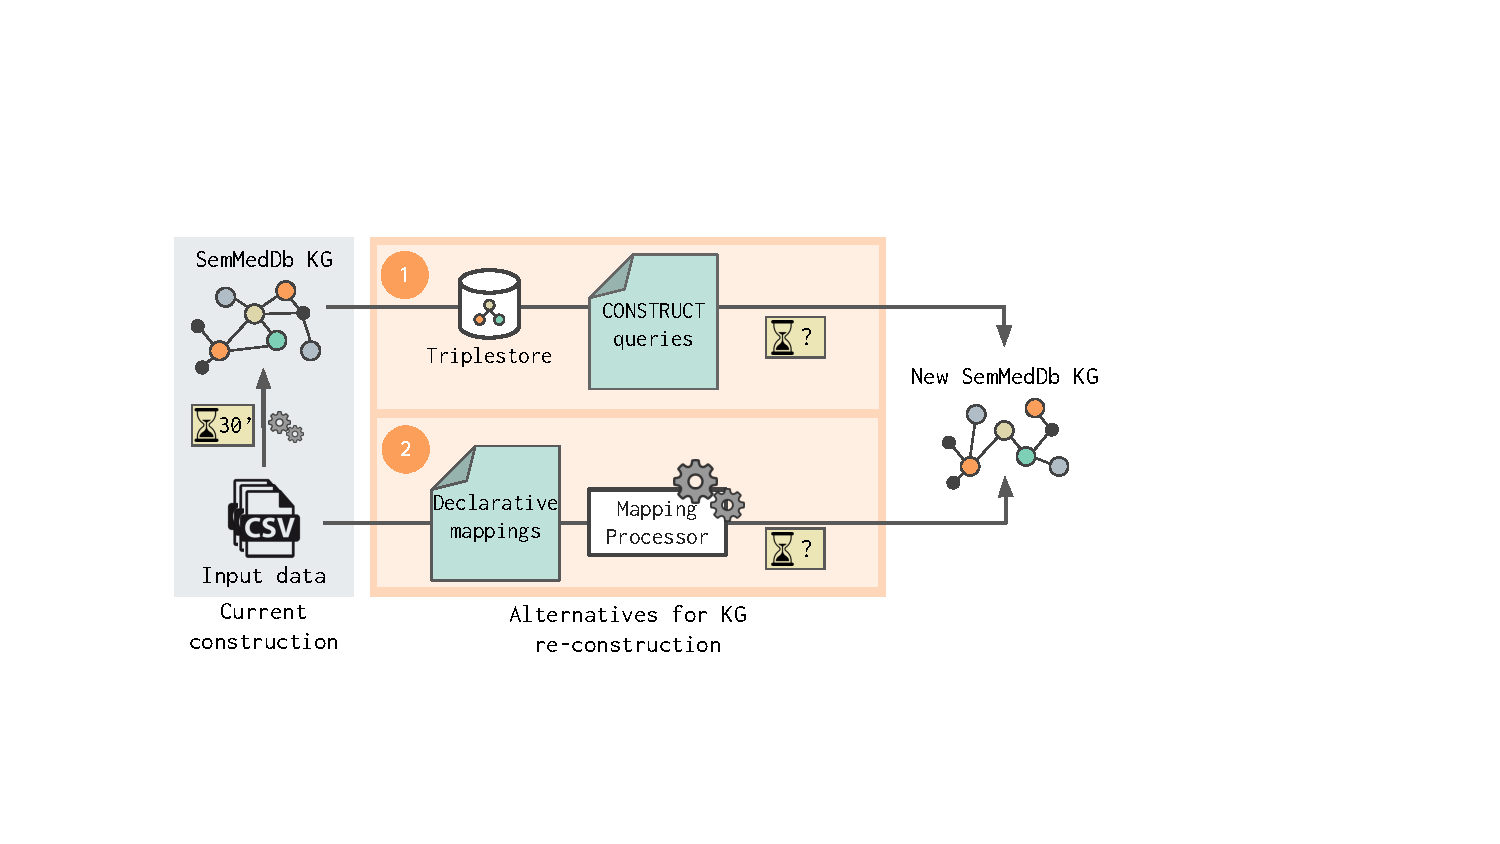
\includegraphics[width=1\linewidth]{figures/chp6-1_motivating-example.pdf}
    \caption[KG re-construcion alternatives]{Alternatives for re-constructing a pre-existing knowledge graph.}
    \label{fig:chp6-1_mot-example}
\end{figure}

Consider the SemMedDB dataset, that contains entities extracted from biomedical texts, as well as the semantic types of these concepts and a timestamp of when they were extracted. A stable version of a knowledge graph represents this information, where the timestamp and semantic type are related to its correspondent entity with an N-Ary relationship. However, the maintainers of this knowledge graph want to reduce the size of the graph by reducing the number of nodes, as well as to represent this information with RDF-star to start adopting the RDF 1.2 specification.

The graph maintainers have access to the original source data, so they can change the original KG construction pipeline, that uses declarative mappings to construct the graph. However, since this graph is not going to be updated with new data, it is also possible to change the structure of the graph with queries within the triplestore where it is maintained. They know the time it takes to generate the graph in its original representation. However, they are not certain whether generating the graph in the new representation using this pipeline will take more time, or if with queries the transformation could be performed faster (\cref{fig:chp6-1_mot-example}). Hence, the objective of this work consist of assessing the aspects that influence this situation to help in making an informed decision.


\section{Methodology}
\label{sec:chp6-1_methodology}

In this section we present the methodology followed to analyze the impact of different approaches for re-constructing knowledge graphs from a reification perspective. More in detail, we compare two ways of re-structuring a KG to change its reification approach, (i) with declarative mapping technologies from scratch (e.g., RML~\citep{Dimou2014rml,iglesias2023rml}) and (ii) with \texttt{CONSTRUCT} queries in a triplestore from the previous version of the graph. We aim to answer the following research questions: \ana{ojo a esto para cuando estén los objetivos y demás escritos }
\textbf{(RQ1)} In which cases is it more efficient in terms of time to either construct a reified knowledge graph from the original data sources or to re-construct it within a triplestore?
\textbf{(RQ2)} Which of these two approaches is more scalable as the size of the data increases?
\textbf{(RQ3)} What is the impact of the different reification representations on triplestores and mapping processors?
%In this section, we describe the experimental configuration for the evaluation carried out to answer these research questions. 
All resources to reproduce the experiments are available on GitHub.\footnote{\url{https://github.com/oeg-upm/kg-reconstruction-eval}}



\subsection{Dataset}
\label{sec:chp6-1_dataset}

\ana{ojo que esta sección es como para la de rml-star}

We use the Semantic MEDLINE Database (SemMedDB)~\citep{SemMedDB} in the experimental evaluation. This database consists of a repository with biomedical entities and relationships (subject-predicate-object) extracted from biomedical texts.
%, mainly titles and abstracts from PubMed citations. 
This dataset is available as a relational database and CSV files.\footnote{\url{https://lhncbc.nlm.nih.gov/ii/tools/SemRep\_SemMedDB\_SKR/SemMedDB\_down\-load.html}}
It is licensed under the UMLS - Metathesaurus License Agreement,\footnote{\url{https://www.nlm.nih.gov/research/umls/knowledge\_sources/metathesaurus/release\-/license\_agreement.html}} which does not allow its distribution, but it may be accessed with an account with the UMLS license.\footnote{An account with the UMLS license can be requested at \url{https://www.nlm.nih.gov/databases/umls.html}.}


We use the CSV files for (i)~\textit{entity} predictions (from ENTITY.csv), and (ii)~\textit{predication} predictions (from PREDICATION.csv and PREDICATION\_AU\-X.csv). Listings~\ref{lst:chp6-1_semmeddb_entity},~\ref{lst:chp6-1_semmeddb_pred} and~\ref{lst:chp6-1_semmeddb_predaux} illustrate the columns used from the files with synthetic data.
For \textit{predications}, only data for \textit{subjects} is shown; the missing columns regarding \textit{objects} follow the same structure as \textit{subjects}.
%This data contains information on predicted entities and predicted subject-predicate-object predications.
\textit{Subjects} and \textit{objects} (from \textit{predications}), and \textit{entities} are assigned a \textit{semantic type} with a confidence score.
These \textit{semantic types} categorize the extracted concept in the biomedical domain.\footnote{\url{https://www.nlm.nih.gov/research/umls/new\_users/online\_learning/SEM\_003.html}}
In addition, the extraction of \textit{subjects} and \textit{objects} is assigned a timestamp on when it took place. 
Thus, the score and timestamp represent metadata about other statements, which are fit to represent using reification.

We model this tabular dataset as five annotated statements: 
Three assign \textit{semantic types} to \textit{subjects}, \textit{objects}, and \textit{entities} with a confidence score; and two provide the timestamp for the extraction of \textit{subjects} and \textit{objects} from text.  


\noindent\begin{minipage}{0.42\linewidth}
\begin{captionedlisting}{lst:chp6-1_semmeddb_entity}{ENTITY.csv snippet.}
\centering
\begin{tabular}{c}
\hspace{-0.7em}
{
\begin{lstlisting}[basicstyle=\ttfamily\small,label={lst:chp6-1_semmeddb_entity},columns=flexible]
ENTITY_ID , SEMTYPE , SCORE
12345      , orga     , 790
\end{lstlisting}
}
\end{tabular}
\end{captionedlisting}
\end{minipage}
\,\,\,\,\hfill
\begin{minipage}{0.58\linewidth}
\begin{captionedlisting}{lst:chp6-1_semmeddb_pred}{PREDICATION.csv snippet.}
\centering
\begin{tabular}{c}
\hspace{-1em}
{
\begin{lstlisting}[basicstyle=\ttfamily\small,label={lst:chp6-1_semmeddb_pred},columns=flexible]
PREDICATION_ID , SUBJ_SEMTYPE , SUBJ_NAME
13579            , Semtype       , SubjName
\end{lstlisting}
}
\end{tabular}
\end{captionedlisting}
\end{minipage}

\noindent\hspace{0.23\linewidth}\begin{minipage}{\linewidth}
\begin{captionedlisting}{lst:chp6-1_semmeddb_predaux}{PREDICATION\_AUX.csv snippet.}
\centering
\begin{tabular}{c}
\hspace{-7em}
{
\begin{lstlisting}[basicstyle=\ttfamily\small,label={lst:chp6-1_semmeddb_predaux},columns=flexible]
PREDICATION_AUX_ID , PREDICATION_ID , SUBJ_SCORE , TIMESTAMP
67890                , 13579            , 800         , 1651740766
\end{lstlisting}
}
\end{tabular}
\end{captionedlisting}
\end{minipage}


To test the scalability of the evaluated approaches, we subset this dataset into four sizes taking as input from the abovementioned CSV files with (i)~1K rows, (ii)~10K rows, (iii)~100K rows and (iv)~1M rows. The number of triples produced for each reification version in each scale is shown in \cref{tab:chp6-1_data-triple-number}.

\begin{table}[t]
\caption[SemMedDB scale sizes]{Number of triples of the SemMedDB graph in the selected representations for each scale.}
\label{tab:chp6-1_data-triple-number}
\centering
\begin{tabular}{cccccc}
    \cmidrule{2-6}
    & & \textbf{1K} & \textbf{10K} & \textbf{100K} & \textbf{1M} \\ \midrule
    \textbf{Standard Reification} & & 25,000 & 249,997 & 2,499,966 & 24,999,607 \\ \midrule
    \textbf{Named Graphs} & & 10,000 & 99,994 & 999,932 & 9,999,190 \\ \midrule
    \textbf{N-Ary Relationships} & & 15,000 & 149,997 & 1,499,966 & 14,999,595 \\ \midrule
    \textbf{RDF-star} & & 8,485 & 78,655 & 710,588 & 6,503,388 \\ \bottomrule
\end{tabular}
\end{table}




\subsection{Mappings and Queries}
\label{sec:chp6-1_map-queries}
The following resources are used: 
(i)~a set of declarative mappings that are used for constructing the knowledge graph from the SemMedDB tabular files in the four selected reification representations; and (ii)~a set of SPARQL queries that are used for re-constructing the graph within different triplestores. A summary of their characteristics is shown in \cref{tab:chp6-1_mapping-char}.

We use two sets of mappings, one set written in the RML mapping language~\citep{iglesias2023rml}, and the other in SPARQL-Anything~\citep{asprino2023sparql-anything}. These languages allow describing transformation of heterogeneous data sources into RDF following the schema provided by an ontology or vocabulary, and are processed by different engines (see \cref{sec:chp6-1_engines}). Each set of mappings is comprised of four mappings, to construct the knowledge graphs in the four representations selected (i.e. Standard Reification, N-Ary Relationships, Named Graphs and RDF-star).


RML extends the R2RML Recommendation~\citep{das2012r2rml} to describe more data sources besides Relational Databases. RML rules are grouped within \textit{Triples Maps}, which contain one \textit{Logical Source}, one \textit{Subject Map} and zero to multiple \textit{Predicate Object Maps}. \textit{Logical Sources} describe the input data to be transformed. \textit{Subject Maps} indicates how the subjects of the triples are created, while \textit{Predicate Object Maps} specify how the predicates and objects of the triples are created. \cref{lst:chp6-1_rml-star} shows an example of a mapping that generates in RDF-star the annotation of the semantic types of \textit{entities} with a score from the CSV file shown in \cref{lst:chp6-1_semmeddb_entity}. This mapping uses the RML-star module~\citep{delva2021rml-star,iglesias2023rml} to generate RDF-star graphs, which allows RML to quote \textit{Triples Map} with the \texttt{rml:quotedTriplesMap} property. For these mappings, we show the number of sets of rules (i.e. \textit{Triples Map}) and  \textit{Predicate Object Maps} specified (\cref{tab:chp6-1_mapping-char}).

\noindent\begin{minipage}{1\linewidth}
\begin{captionedlisting}{lst:chp6-1_rml-star}{RML-star mapping snippet to create the RDF-star graph for \textit{entity} from data in \cref{lst:chp6-1_semmeddb_entity}. }
\centering
\begin{tabular}{cc}
{\begin{lstlisting}[basicstyle=\ttfamily\small,label={list:example1}]
<#Entity> 
 a rml:TriplesMap ;
 rml:logicalSource [
  rml:source "ENTITY.csv"
 ];
 rml:subjectMap [
  rml:template ":{ENTITY_ID}"
 ];
 rml:predicateObjectMap [
  rml:predicate :semanticType;
  rml:objectMap [
   rml:reference "SEMTYPE"
  ] ] .
\end{lstlisting}}
&
%\hspace{3em}
{\begin{lstlisting}[basicstyle=\ttfamily\small,label={list:example1},numbers=right,firstnumber=13]
<#EntityScore> 
  a rml:AssertedTriplesMap ;
 rml:logicalSource [
  rml:source "ENTITY.csv"
 ];
 rml:subjectMap [
  rml:quotedTriplesMap <#Entity>;
 ];
 rml:predicateObjectMap [
  rml:predicate :score ;
  rml:objectMap [
   rml:reference "SCORE"
  ] ] .
\end{lstlisting}}

\end{tabular}
\end{captionedlisting}
\end{minipage}


\begin{table}[t!]
    \caption[Characteristics of evaluation mapping]{Characteristics of mappings in RML and SPARQL-Anything. \#TM stands for number of Triples Map, \#POM for Predicate Object Map, and \#TP for Triple Patterns. The shown operators appear usually in the \texttt{WHERE} clause; the ones marked with $^c$ appear in the \texttt{CONSTRUCT} clause. }
    \label{tab:chp6-1_mapping-char}
    \centering
    \begin{tabular}{ccc|cc}
        \cmidrule{2-5}
         & \multicolumn{2}{c|}{\textbf{RML}} & \multicolumn{2}{c}{\textbf{SPARQL-Anything}}  \\ \midrule
         & \textbf{\#TM} & \textbf{\#POM} & \textbf{\#TP$^c$} & \textbf{Additional operators}  \\ \midrule
         \textbf{Standard Reification} & 9 & 20 & 25 & UNION, BIND  \\ \midrule
         \textbf{Named Graphs} & 10 & 10 & 10 & UNION, BIND, GRAPH$^c$  \\ \midrule
         \textbf{N-Ary Relationships} & 13 & 15 & 15 & UNION, BIND  \\ \midrule
         \textbf{RDF-star} & 10 & 10 & 10 & UNION, BIND  \\  \midrule
         
    \end{tabular}
\end{table}

SPARQL-Anything heavily relies on the SPARQL syntax, overriding the \texttt{SERVICE} operator while leveraging the rest of its features. This operator is then always present in the queries and hence is not shown in the table. The graphs are built with \texttt{CONSTRUCT} clauses. \cref{lst:chp6-1_sparql-anything} shows a mapping example that generates in RDF-star the annotation of the semantic types of \textit{entities} with a score from the CSV file shown in \cref{lst:chp6-1_semmeddb_entity}.
For each mapping, we show the number of triple patterns in this clause and additional SPARQL clauses (\cref{tab:chp6-1_mapping-char}). All mappings contain the same number of triple patterns in the \texttt{WHERE} clause.




\noindent\begin{captionedlisting}{lst:chp6-1_sparql-anything}{SPARQL-Anything mapping snippet to create the RDF-star graph for \textit{entity} from data in \cref{lst:chp6-1_semmeddb_entity}.  }
\centering
{
\begin{lstlisting}[basicstyle=\ttfamily\small,label={list:example1},columns=flexible,language=sparql]
CONSTRUCT {
  ?entity_id_iri :semanticType ?entity_semtype .
  << ?entity_id_iri :semanticType ?entity_semtype >> :score ?entity_score .
 } WHERE {
  {  SERVICE <x-sparql-anything:location=./data/entity.csv>
   { [] xyz:ENTITY_ID ?entity_id;
     xyz:SEMTYPE ?entity_semtype;
     xyz:SCORE ?entity_score;
    BIND(uri(concat(str("http://semmeddb.com/entity/"),
                        encode_for_uri(?entity_id))) as ?entity_id_iri)
   }  } }

\end{lstlisting}
}
\end{captionedlisting}



SPARQL queries use the \texttt{CONSTRUCT} clause to re-construct a given graph represented with one of the reifications into the other three representations. We use twelve queries to transform all pairs of representations, whose characteristics are shown in \cref{tab:chp6-1_query-char}. We show for each query the number of triple patterns in the \texttt{WHERE} and \texttt{CONSTRUCT} clauses, and the additional operators used. Except for \texttt{GRAPH}, the rest of operators only appear within the \texttt{WHERE} clause. An example of a query is shown in \cref{lst:chp6-1_sparql-construct}, which generates RDF-star from Named graphs.


\noindent\begin{captionedlisting}{lst:chp6-1_sparql-construct}{SPARQL query snippet to create the RDF-star graph from the Named Graphs representation for \textit{entity}. }
\centering
{
\begin{lstlisting}[basicstyle=\ttfamily\small,label={list:example1},columns=flexible,language=sparql]
CONSTRUCT  {
  ?entity_id_iri :semanticType ?entity_semtype .
  << ?entity_id_iri :semanticType ?entity_semtype >> :score ?entity_score .
} WHERE {
  GRAPH ?entity_graph_iri { ?entity_id_iri :semanticType ?entity_semtype }
  ?entity_graph_iri :score ?entity_score . 
}
\end{lstlisting}
}
\end{captionedlisting}



\begin{table}[t!]
\caption[Characteristics of evaluation SPARQL queries]{Characteristics of the SPARQL queries used for the evaluation to transform the graph from a \textit{source} representation to a \textit{target} representation. \#TP stands for the number of triple patterns. Fields marked with $^c$ appear in the \texttt{CONSTRUCT} clause, while $^w$ indicates the \texttt{WHERE} clause. }
\centering
\label{tab:chp6-1_query-char}
\resizebox{\columnwidth}{!}
{\begin{tabular}{cccccccccc}
    \cmidrule{2-10}
 & \textbf{Source} & \textbf{Target} & \textbf{\#TP$^w$} & \textbf{\#TP$^c$} & \textbf{UNION$^w$} & \textbf{BIND$^w$} & \textbf{FILTER$^w$} & \textbf{VALUES$^w$} & \textbf{GRAPH}  \\ \midrule
\textbf{Q1} & \multirow{4}{*}{\textbf{N-AryRel.}} & \textbf{Std. Reif.} & 6 & 10 & \checkmark &  &  & \checkmark &  \\ \cmidrule{3-10}
 \textbf{Q2} & & \textbf{RDF-Star} & 6 & 4 & \checkmark &  &  & \checkmark &  \\ \cmidrule{3-10}
 \textbf{Q3} & & \textbf{Named Graphs} & 6 & 4 & \checkmark &  &  & \checkmark & \checkmark $^c$ \\ \midrule
\textbf{Q4} & \multirow{4}{*}{\textbf{Std. Reif.}} & \textbf{RDF-star} & 8 & 4 & \checkmark &  &  & \checkmark &  \\ \cmidrule{3-10}
 \textbf{Q5} & & \textbf{N-Ary Rel.} & 20 & 15 & \checkmark &  & \checkmark &  &  \\ \cmidrule{3-10}
 \textbf{Q6} & & \textbf{Named Graphs} & 8 & 4 & \checkmark &  &  & \checkmark & \checkmark $^c$ \\ \midrule
\textbf{Q7} & \multirow{4}{*}{\textbf{RDF-star}} & \textbf{Std. Reif.} & 5 & 25 & \checkmark & \checkmark & \checkmark &  &  \\ \cmidrule{3-10}
 \textbf{Q8} & & \textbf{N-Ary Rel.} & 5 & 15 & \checkmark & \checkmark & \checkmark &  & \\ \cmidrule{3-10}
 \textbf{Q9} & & \textbf{Named Graphs} & 5 & 10 & \checkmark & \checkmark & \checkmark &  & \checkmark $^c$ \\ \midrule
\textbf{Q10} & \multirow{4}{*}{\textbf{Named Graphs}} & \textbf{Std. Reif.} & 4 & 10 & \checkmark &  &  & \checkmark & \checkmark $^w$ \\ \cmidrule{3-10}
 \textbf{Q11} & & \textbf{RDF-Star} & 4 & 4 & \checkmark &  &  & \checkmark & \checkmark $^w$ \\ \cmidrule{3-10}
 \textbf{Q12} & & \textbf{N-Ary Rel.} & 4 & 15 & \checkmark &  &  & \checkmark & \checkmark $^w$  \\  \bottomrule
\end{tabular}}
\end{table}



\subsection{Engines}
\label{sec:chp6-1_engines}
We choose a set of 2 mapping processors and 3 triplestores to be representative in our evaluation, while focusing on open-source tools. The selected mapping processors, Morph-KGC (v2.5.0)~\citep{arenas2022morphkgc} and SPARQL-Anything (v0.8.1)~\citep{asprino2023sparql-anything} are the systems with a stable version capable of producing RDF-star at the time of writing this paper. The SDM-RDFizer~\citep{iglesias2020rdfizer} is in the process of implementing this feature, but no stable version has been released yet. Regarding triplestores, we use the free version of GraphDB (v10.2.1), and the open-source Jena Fuseki (v4.8.0) and Oxigraph (v0.3.16). While GraphDB and Jena Fuseki store the graph in physical memory, Oxigraph performs the queries in memory. All engines perform duplicate removal in the results by default, with the exception of Oxigraph. For this triplestore, we add and measure a second step of duplicate removal with BASH commands.


We did attempts to include Virtuoso in the evaluation; however, several issues raised. The number of queries this triplestore can perform is very limited in this evaluation (only 4 from 12): This triplestore
does not implement RDF-star yet, and cannot produce named graphs declared inside the \texttt{CONSTRUCT} clause. In addition, Virtuoso limits the number of triples that can be produced with this clause to 1M.\footnote{\url{https://lig-membres.imag.fr/rousset/publis/tess.pdf}} When this limit is removed, an error appears that impedes the writing of the result in a file when it is large, which has been unsolved for years.\footnote{\url{https://github.com/openlink/virtuoso-opensource/issues/11}} 




\subsection{Experimental setup and Metrics}
\label{sec:chp6-1_exp-setup}
We perform the evaluation in two steps. First, the KG construction system evaluation is run, taking as input the SemMedDb dataset in CSV format and the mappings, and producing the corresponding RDF datasets in the four selected representations. Then, the triplestore evaluation is carried out, taking as input the produced datasets in the KG construction system evaluation, and producing RDF datasets in another representation.


We measure the \textit{materialization time} to construct the RDF graph from the input data sources in KG construction systems.
For triplestores, we measure \textit{query execution time} as the total time from query execution until the complete answer is generated. 
We also report the geometric mean of all queries that generate the same reified RDF graph, similar to previously used by~\citep{morsey2011dbpedia,schmidt2009sp}. 
The \textit{geometric mean} reports the central tendency of all execution times for a set of queries, reducing the effect of outliers. 
With this metric, we provide a general measurement of the performance of each triplestore when generating graphs in each representation. 
This allows an easier comparison with the KG construction systems. 
We run every experiment 5 times with a timeout of 24h, measure the time and calculate the median.
We run all experiments over an Ubuntu 20.04 server with
32 cores Intel(R) Xeon(R) Gold 5218R CPU @ 2.10GHz
102400 Mb RAM RDIMM, 3200 MT/s and 
100 Gb HD SSD 6 Gb/s. 




\section{Results}
\label{sec:chp6-1_results}


\begin{figure}[t!]
    \centering
    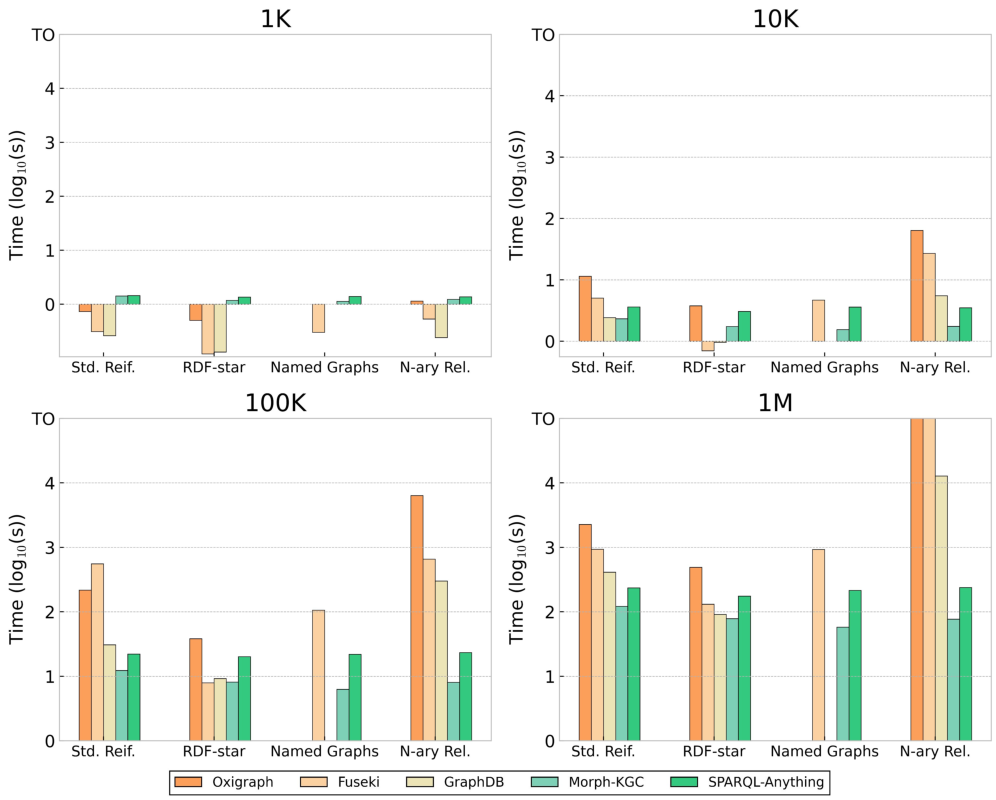
\includegraphics[width=\linewidth]{figures/chp6-1_results-map-queries.pdf}
    \caption[Overall execution times of KG re-construction evaluation]{Execution time for KG construction engines with declarative mappings, and triplestores with SPARQL queries. The results for the triplestores are grouped by the \textit{target} representation.}
    \label{fig:chp6-1_map-queries}
\end{figure}




The results of the evaluation performance are shown in Figs. \ref{fig:chp6-1_map-queries} and \ref{fig:chp6-1_queries}. \cref{fig:chp6-1_map-queries} reports the comparison between knowledge graph construction systems using declarative mappings, and triplestores with SPARQL queries. For the latter, the geometric mean of the query execution time for all queries that generate each representation is provided. \cref{fig:chp6-1_queries} reports a fine-grained comparison of the performance of each triplestore on the proposed queries that perform translations between each combination of pairs of representations.

Focusing on the comparison between triplestores and KG construction systems (\cref{fig:chp6-1_map-queries}), we generally observe that for small data sizes, triplestores obtain better results, while KG construction systems scale better as data size increases. However, in the case of producing RDF-star, Fuseki and GraphDB are competitive w.r.t. SPARQL-Anything or Morph-KGC. These triplestores obtain better results for the scales 1K and 10K, and similar ones for 100K and 1M. Additionally, despite the variety in mapping characteristics, neither Morph-KGC nor SPARQL-Anything seem to be highly affected by the different representations, as opposed to the triplestores. The differences are not remarkable, but in general Morph-KGC generates the fastest Names Graphs, in contrast with SPARQL-Anything, which performs better with RDF-star. For triplestores, producing N-Ary Relationships and Standard Reification is more costly than the other representations. Another relevant point to consider is that SPARQL 1.1 does not allow \texttt{GRAPH} clause within the \texttt{CONSTRUCT} operator. Thus, only Fuseki, which implements this extension natively, can generate the Named Graphs datasets.

Comparing the behavior of engines that perform the same task, GraphDB overcomes Fuseki and Oxigraph for SPARQL queries, while Morph-KGC reports better results than SPARQL-Anything for KG construction from heterogeneous data sources, as was reported in previous works~\citep{arenas2023morphstar}.
For small data sizes, GraphDB and Fuseki perform similar, while Oxigraph reports higher query execution time. This is because Oxigraph loads the complete RDF graph in memory and the physical data structures from Fuseki and GraphDB speed up query execution time. In larger datasets, GraphDB generally scales better than Fuseki, which for example, reports a timeout for generating N-Ary Rel. in scale 1M. 

%Answering the research questions, we can say that triplestores perform faster for small sizes (\textbf{RQ1}), while KG construction systems present a more robust behaviour with increasing data size (\textbf{RQ2}). In addition, triplestores are more influenced by the changes in representations, whereas KG construction systems are mostly unaffected (\textbf{RQ3}).

 


\begin{figure}[t!]
    \centering
    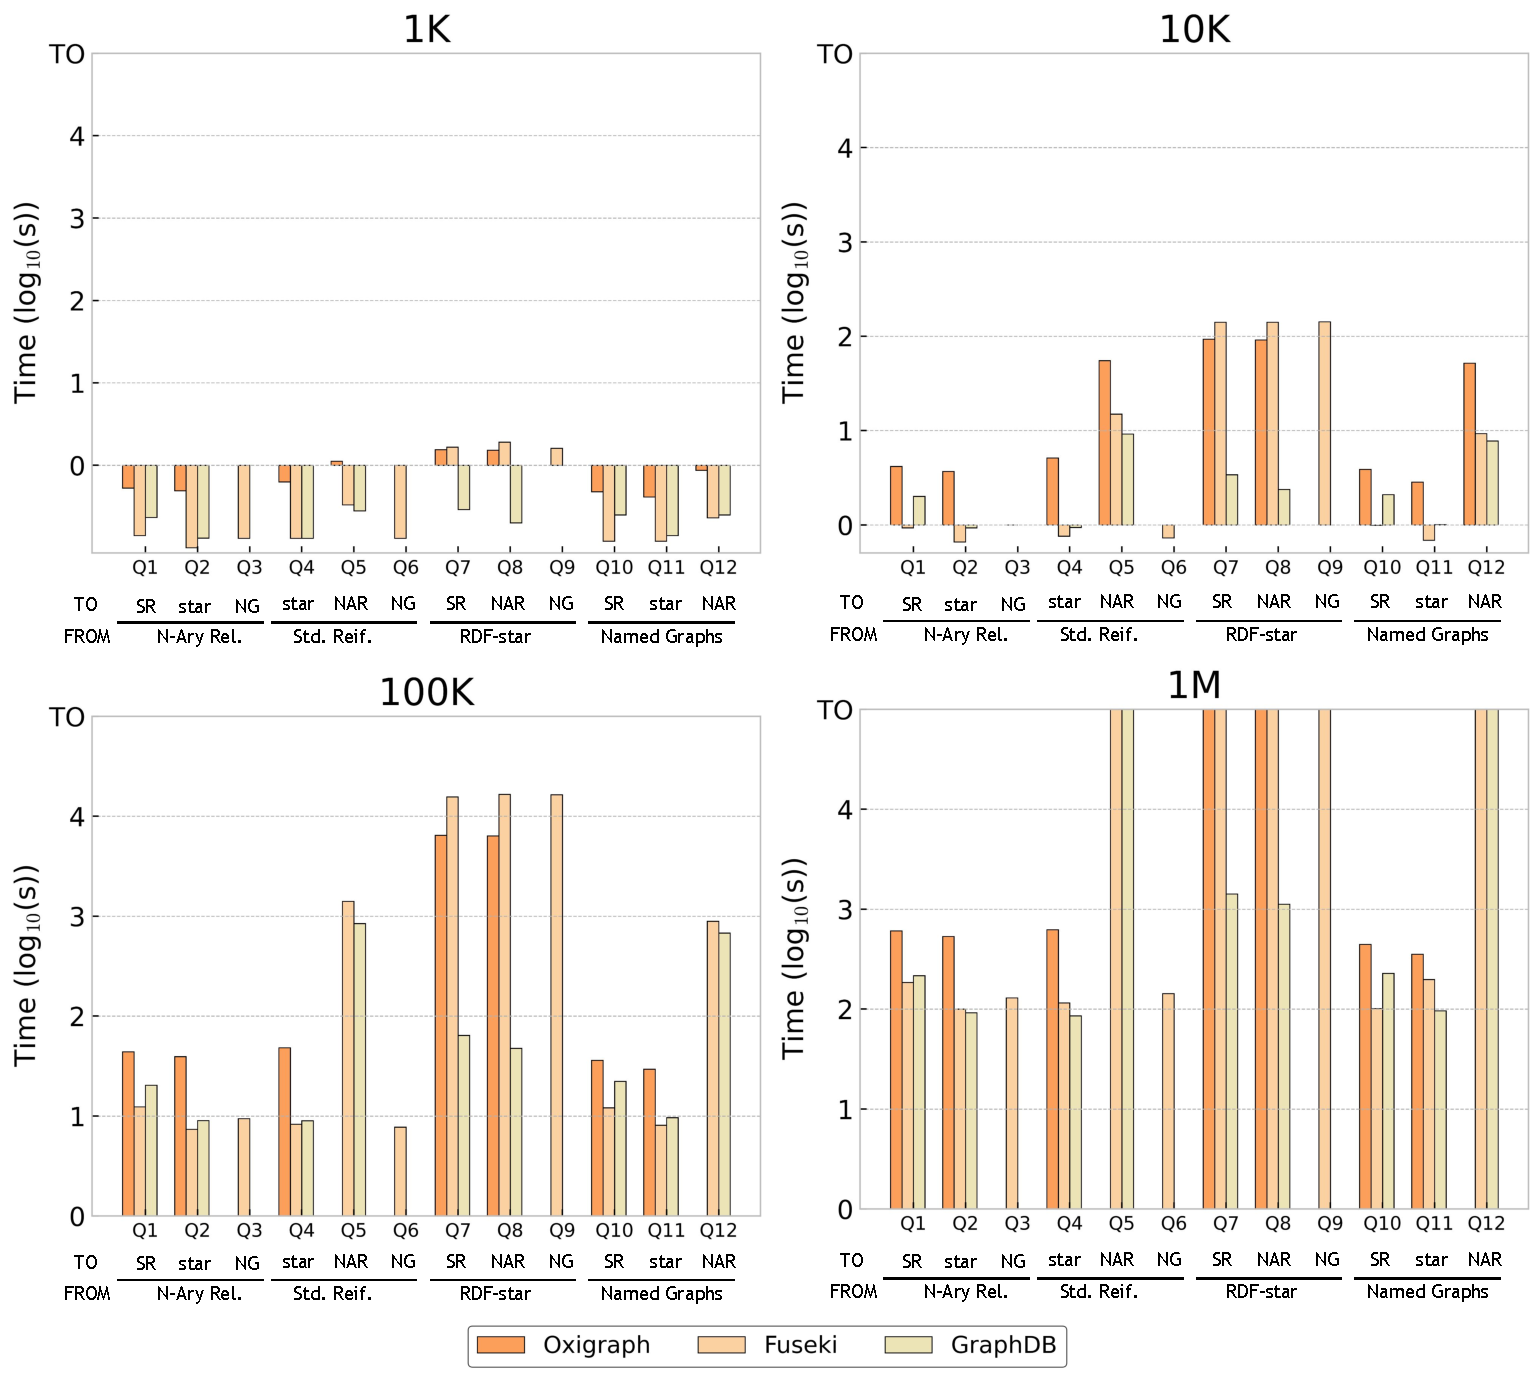
\includegraphics[width=\linewidth]{figures/chp6-1_results-queries.pdf}
    \caption[Execution times of KG re-construction in triplestores]{Execution time of triplestores with the SPARQL queries that perform translations for pairs of representations.}
    \label{fig:chp6-1_queries}
\end{figure}


Looking into the particular differences of the pairs of translation performed with triplestores, we can observe in more detail how the different reification models affect the performance of the graph re-construction with \texttt{CONSTRUCT} queries. \cref{fig:chp6-1_queries} present the results grouping the queries in the legend by the \textit{source} reification representation (i.e. from which representation the dataset is transformed). 

Queries with RDF-star as the source representation (Q7-Q9) generally perform the worst on every scale. This set of queries includes additional SPARQL operators that are usually not required in the rest of queries: \texttt{BIND} and \texttt{FILTER}. Additionally, the recursiveness of the model, together with the fact that it is the only one that makes structural changes over RDF, can produce a negative impact on the performance of the transformation queries. Only GraphDB manages these queries better compared to the other triplestores, reporting better results, while the others reach the time limit in scale 1M. It generates the graph faster than Oxigraph and Fuseki, while it is just slightly slower compared to the queries with other source representations. This may suggest that the additional operators are not the main responsible for the increase of time processing, but the inner performance of the triplestore w.r.t. RDF-star.

The behavior of the construction of N-Ary Relationships is also remarkable. Independently of the source model, it is more costly to produce it than the other models. Queries Q5 and Q12 report an out-of-memory error in Oxigraph for scales 100K and 1M, while reaching timeout in Fuseki and GraphDB in scale 1M. Query Q9 is more affected by the source representation, RDF-star, than the target, thus the result for this query is similar to the ones affected by the abovementioned issue of this model as source. 
Only in GraphDB, Q9 reports less time to produce N-Ary Relationship than Standard Reification, which may be due to having fewer triple patterns to construct (see \cref{tab:chp6-1_query-char}). Interestingly, query Q5 involves an additional operator (\texttt{FILTER}) and more triple patterns than Q4 and Q6, which may explain its low performance. However, query Q12 does not involve any additional operators w.r.t. Q10 and Q11, and has only a few more triple patterns, which does not seem enough justification for its poor performance. Looking at the queries, both Q5 and Q12 contain five joins. Their presence is more likely to be the reason why they take up to two magnitude orders more in the result time than the queries that share source representation. 


%%%%% This one is smaller but visually I think the other (below) is more understandable
%\begin{table}[t!]
%\caption{Geometric mean of the query result times (s) from all triplestores grouping by \textit{source} representation and \textit{target} representation. The lowest times are highlighted in \textbf{bold}, while the highest are %\underline{underlined}.}
%\centering
%\label{tab:closeup-queries}
%\resizebox{\columnwidth}{!}
%{\begin{tabular}{ccccc|cccc}
%    \cmidrule{2-9}
%    & \multicolumn{4}{c|}{\textbf{Source}} & \multicolumn{4}{c}{\textbf{Target}} \\ \midrule
%    \multicolumn{1}{c|}{\textbf{Scale}} & \textbf{Std. Reif.} & \textbf{RDF-star}  & \textbf{N-Graphs} & \textbf{N-Ary Rel.} & \textbf{Std. Reif.} & \textbf{RDF-star}  & \textbf{N-Graphs} & \textbf{N-Ary Rel.} \\ \midrule
%    \multicolumn{1}{c|}{1K} & 0.283 & \underline{0.952} & 0.260 & \textbf{0.204} & 0.387 & \textbf{0.199} & 0.303 & \underline{0.526} \\ \midrule
%    \multicolumn{1}{c|}{10K} & 4.126 & \underline{40.981} & 3.395 & \textbf{1.505} & 5.200 & \textbf{1.366} & 4.693 & \underline{21.218} \\ \midrule
%    \multicolumn{1}{c|}{100K} & 56.612 & \underline{2449.544} & 43.756 & \textbf{16.040} & 154.728 & \textbf{14.066} & 106.176 & \underline{1078.092} \\ \midrule
%    \multicolumn{1}{c|}{1M} & 1085.228 & \underline{15738.107} & 773.737 & \textbf{205.407} & 954.710 & \textbf{180.384} & 927.741 & \underline{28788.048} \\   \bottomrule
%    \end{tabular}}
%\end{table}


%%%% transposed table, occupies more space
\begin{table}[t!]
\caption[Execution time results for re-construction evaluation with triplestores]{Geometric mean of the query result times (s) from all triplestores grouping by \textit{source} representation and \textit{target} representation. The lowest times are highlighted in \textbf{bold}, while the highest are \underline{underlined}.}
\centering
\label{tab:chp6-1_closeup-queries}
\begin{tabular}{cccccc}
    \cmidrule{2-6}
 & \textbf{Representation} & \textbf{1K} & \textbf{10K} & \textbf{100K} & \textbf{1M} \\ \midrule
 \multirow{5}{*}{\textbf{Source}} & \textbf{Std. Reif.} & 0.283 & 4.126 & 56.612 & 1085.228  \\ \cmidrule{2-6}
  & \textbf{RDF-Star} & \underline{0.952} & \underline{40.981} & \underline{2449.544} & \underline{15738.107}  \\ \cmidrule{2-6}
  & \textbf{Named Graphs} & 0.260 & 3.395 & 43.756 & 773.737 \\ \cmidrule{2-6}
 & \textbf{N-Ary Rel.} & \textbf{0.204} & \textbf{1.505} & \textbf{16.040} & \textbf{205.407}  \\ \midrule
 \multirow{5}{*}{\textbf{Target}} & \textbf{Std. Reif.} & 0.387 & 5.200 & 154.728 & 954.710  \\ \cmidrule{2-6}
  & \textbf{RDF-Star} & \textbf{0.199} & \textbf{1.366} & \textbf{14.066} & \textbf{180.384} \\ \cmidrule{2-6}
  & \textbf{Named Graphs}  & 0.303 & 4.693 & 106.176 & 927.741 \\ \cmidrule{2-6}
 \ & \textbf{N-Ary Rel.} & \underline{0.526} & \underline{21.218} & \underline{1078.092} & \underline{28788.048} \\   \bottomrule
\end{tabular}
\end{table}

\cref{tab:chp6-1_closeup-queries} shows a summary of the results from the triplestores grouped by \textit{source} and \textit{target} representation. In general, RDF-star is the fastest representation to construct, while becoming highly inefficient when acting as the source representation. Hence, most of the triplestores do not seem yet optimized to process it. On the contrary, N-Ary relationships perform the fastest being the source representation, but it requires performing joins in the \texttt{CONSTRUCT} that make it the least suitable as a target representation. Standard Reification and Named Graphs perform more consistently overall. Named Graphs take less time than Standard Reification as source and target representation, but can only be generated with Fuseki. 

%Answering \textbf{RQ3}, the combination of representations highly influences the behavior of the triplestores, both in the \texttt{WHERE} and \texttt{CONSTRUCT} clauses. It is especially remarkable for RDF-star and N-Ary Relationships. RDF-star is the fastest representation to generate, but performs the slowest being the source representation; while N-Ary Relationships present the exact opposite behavior. Named Graphs and Standard Reification report a more consistent behavior.




\section{Discussion}
\label{sec:chp6-1_discussion}

This section addresses the following question: given a knowledge graph where reificaiton is needed, is it faster to construct it from the original data sources with the new representation, or to re-construct it within a triplestore?\ana{ojo esta frase, cuadrar con objetivos/RQ cuando estén } To answer this question, we perform an empirical analysis using two KG construction engines and three triplestores, performing the re-construction with four data sizes in four different reification models: RDF-star, Standard Reification, N-Ary Relationships and Named Graphs. Our results show that KG construction engines in general are more scalable, almost independently of the kind of reification. Triplestores perform best for small data sizes. However, their performance is highly dependent on the source representation (in the \texttt{WHERE} clause) and the target representation (in the \texttt{CONSTRUCT} clause). The time for producing RDF-star and Named Graphs is competitive with the KG construction approach. Yet, this approach becomes inefficient for producing N-Ary Relationships due to the need of introducing more joins in the \texttt{CONSTRUCT} clause; and when RDF-star is the source model, since most triplestores are not optimized for its new syntax. 

%%%%%%%%%%%%% SUMMARY AND MAIN CONCLUSIONS %%%%%%%%%%%%
Our evaluation shows that the KG construction engines are more robust for increasing data size and changing the reification models. Performing the re-construction in the triplestore is suitable for small data sizes, but it is largely dependant on the KG structure to offer competitive performance. Thus, we can affirm that performing the re-construction with mappings is in general more reliable, as it is significantly less affected by data size and target representation. 


%%%%%% SPARQL CONSTRUCT rant %%%%%%%
The setup of the evaluation shows us the importance of optimizing SPARQL queries, which gains relevance as the triples to construct increase in number. For instance, the introduction of \texttt{UNION} clauses was needed to avoid costly cartesian products that prevented queries from finishing before the established timeout, or before reaching an out-of-memory error. While this is well known in proficient SPARQL practitioners, it does not come as easily for non-expert users. The performance of SPARQL-Anything, relying almost entirely on SPARQL and Jena processing, is also affected by these different manners of writing the mapping. In contrast, RML mappings are unaffected in this aspect, since how the user writes the mapping does not influence the performance of the compliant systems. SPARQL possess a flexibility and rich expressiveness that languages such as RML lack yet. Nevertheless, it poses the risk for non-expert users to hamper the result retrieval incurring in suboptimal queries. This opens up a challenge for improving the query processing, or even rewriting the queries automatically to be optimized, so as to reduce this accessibility gap for SPARQL.

In addition, this evaluation brings to light that the behavior of the \texttt{CONSTRUCT} clause is not as studied as other SPARQL operators. SPARQL benchmarks often overlook this clause, as it is considered as an extension of \texttt{SELECT}~\citep{schmidt2009sp}. Hence, it is assumed that their performance is comparable and not affected by the change of clause. However, we encountered \texttt{SELECT} queries that returned results in miliseconds, while taking several minutes with \texttt{CONSTRUCT}. 
%% support of GRAPH within CONSTRUCT
%https://stackoverflow.com/questions/59397371/sparql-converting-construct-query-w-named-graph-to-select-query 
This clause also limits the kinds of transformations. For instance, SPARQL 1.1 does not implement generating named graphs (with \texttt{GRAPH}) in \texttt{CONSTRUCT}~\citep{harris2013sparql}.
%\footnote{\url{https://stackoverflow.com/questions/59397371/sparql-converting-construct-query-w-named-graph-to-select-query}}


%%%%%%%%%%% LIMITS OF THE ENGINES %%%%%%%%%%%%
The reported results also open up new challenges for improvement. From the triplestores, only GraphDB could perform reasonably well when RDF-star is the source representation. This highlights the need to continue to improve the processing of this new representation, as it is currently being included in the future RDF 1.2 specification~\citep{hartig2023rdf}. Yet, this representation obtains overall better results when it is the target representation. This will facilitate its adoption, since evolving current KGs into this representation would not suppose an obstacle in terms of performance. 
In addition, all triplestores struggle when the \texttt{CONSTRUCT} clause includes several joins. This fact does not only affect the pairs of transformations studied in this paper, but all potential transformations for evolving knowledge graphs. Regarding KG construction systems, the main challenge still consists of their adoption, as the learning curve for mapping languages is still steep despite efforts to lower it (see \cref{chapter:creation}).


\section{Conclusions}

\ana{mix concluiones de coopis adornadas con las otras}


\chapter{Governing Knowledge Graphs}
\label{chapter:governance}


\chapter{Conclusions and Future work}
\label{chap:conc}


\appendix
%\chapter{Mapeathor Mappings}
\label{sec:appendix-mapeathor}

\begin{captionedlisting}{lst:chp5-1_rml-output}{RML mapping generated with Mapeathor from the spreadsheet shown in Tables \ref{tab:chp5-1_prefix_sheet}, \ref{tab:chp5-1_subject_sheet}, \ref{tab:chp5-1_source_sheet}, \ref{tab:chp5-1_po_sheet} and \ref{tab:chp5-1_function_sheet}. }
\centering
{\begin{lstlisting}[numbers=left,basicstyle=\ttfamily\small,columns=flexible]
@prefix rr: <http://www.w3.org/ns/r2rml#>.
@prefix xsd: <http://www.w3.org/2001/XMLSchema#>.
@prefix rml: <http://semweb.mmlab.be/ns/rml#>.
@prefix ql: <http://semweb.mmlab.be/ns/ql#>.
@prefix rdf: <http://www.w3.org/1999/02/22-rdf-syntax-ns#>.
@prefix ex: <http://ex.com/>.
@prefix grel: <http://semweb.datasciencelab.be/ns/grel#>.
@base <http://example.com/>.

<#PERSON>
    a rr:TriplesMap;
    rml:logicalSource [
    	rml:source "/home/user/data/people.csv";
    	rml:referenceFormulation ql:CSV;
    ];
    rr:subjectMap [
    	a rr:Subject ;
    	rr:termType rr:IRI ;
    	rr:template "http://ex.com/Person/{name}" ;
    	rr:class ex:Person ;
    	rr:class ex:Athlete ;
    ];
    rr:predicateObjectMap [
    	rr:predicateMap	[ rr:constant ex:name];
    	rr:objectMap	[ rml:reference "name"; 
                      rr:termType rr:Literal;  
                      rr:datatype xsd:string;  
                      rr:language "en" ]
    ];
    rr:predicateObjectMap [
    	rr:predicateMap	[ rr:constant ex:plays ];
    	rr:objectMap	[
    		rr:parentTriplesMap	<#SPORT>;
    		rr:joinCondition	[
    			rr:child	"sport_id";
    			rr:parent	"id";
    		];
    	];
    ];
    rr:predicateObjectMap [
      rr:predicateMap	[ rr:constant ex:birthdate] ;
      rr:objectMap	[
    	  rml:functionExecution <#Fun-date> ;
    	  rml:return grel:dateOut ;
    	];
    ]; .

<#SPORT>
    a rr:TriplesMap;
    rml:logicalSource [
    	rml:source "/home/user/data/sports.json";
    	rml:referenceFormulation ql:JSONPath;
        rml:iterator "$\dollar$.*";
    ];
    rr:subjectMap [
    	a rr:Subject ;
    	rr:termType rr:IRI ;
    	rr:template "http://ex.com/Sport/{sport}" ;
    	rr:class ex:Sport ;
    	rr:graphMap [ rr:constant "ex:SportsGraph" ] ;
    ];
    rr:predicateObjectMap [
    	rr:predicateMap	[ rr:constant ex:name];
    	rr:objectMap	[ rml:reference "sport";  
                      rr:termType rr:Literal;  
                      rr:datatype xsd:string;  
                      rr:language "en" ]
    ];
    rr:predicateObjectMap [
    	rr:predicateMap	[ rr:constant ex:code];
    	rr:objectMap	[ rml:reference "id";  
                      rr:termType rr:Literal;  
                      rr:datatype xsd:integer ]
    ]; .

<#Fun-date> a rml:FunctionExecution;
    rml:function grel:toDate ;
    rml:input [
      a rml:Input ;
      rml:parameter grel:valueParam1 ;
      rml:inputValueMap [ rml:reference "birthdate" ];
    ];
    rml:input [
      a rml:Input ;
      rml:parameter grel:valueParam2 ;
      rml:inputValueMap [ rr:constant "dd/MM/yyyy" ];
    ];
    rml:input [
      a rml:Input ;
      rml:parameter grel:valueParam3 ;
      rml:inputValueMap [ rr:constant "yyyy-MM-dd" ];
    ]; .
\end{lstlisting}}
\end{captionedlisting}

\begin{captionedlisting}{lst:chp5-1_r2rml-output}{R2RML mapping generated with Mapeathor from the spreadsheet shown in Tables \ref{tab:chp5-1_prefix_sheet}, \ref{tab:chp5-1_subject_sheet}, \ref{tab:chp5-1_source_sheet}, \ref{tab:chp5-1_po_sheet} and \ref{tab:chp5-1_function_sheet}. }
\centering
{\begin{lstlisting}[numbers=left,basicstyle=\ttfamily\small,columns=flexible]
@prefix rr: <http://www.w3.org/ns/r2rml#>.
@prefix xsd: <http://www.w3.org/2001/XMLSchema#>.
@prefix ql: <http://semweb.mmlab.be/ns/ql#>.
@prefix rdf: <http://www.w3.org/1999/02/22-rdf-syntax-ns#>.
@prefix ex: <http://ex.com/>.
@prefix grel: <http://semweb.datasciencelab.be/ns/grel#>.
@base <http://example.com/>.

<#PERSON>
    a rr:TriplesMap;
    rr:logicalTable [
    	rr:tableName "PEOPLE"
    ];
    rr:subjectMap [
    	a rr:Subject ;
    	rr:termType rr:IRI ;
    	rr:template "http://ex.com/Person/{name}" ;
    	rr:class ex:Person ;
    	rr:class ex:Athlete ;
    ];
    rr:predicateObjectMap [
    	rr:predicateMap	[ rr:constant ex:name];
    	rr:objectMap	[ rr:column "name"; rr:termType rr:Literal; rr:datatype xsd:string; rr:language "en" ]
    ];
    rr:predicateObjectMap [
        rr:predicateMap	[ rr:constant ex:plays ];
        rr:objectMap 	[
            rr:parentTriplesMap <#SPORT>;
            rr:joinCondition	[
                rr:child	"sport_id";
                rr:parent	"id";
            ];
        ];
    ];
.

<#SPORT>
    a rr:TriplesMap;
    rr:logicalTable [
    	rr:tableName "SPORTS"
    ];
    rr:subjectMap [
    	a rr:Subject ;
    	rr:termType rr:IRI ;
    	rr:template "http://ex.com/Sport/{sport}" ;
    	rr:class ex:Sport ;
    	rr:graphMap [ rr:constant "ex:SportsGraph" ] ;
    ];
    rr:predicateObjectMap [
    	rr:predicateMap	[ rr:constant ex:name];
    	rr:objectMap	[ rr:column "sport"; rr:termType rr:Literal; rr:datatype xsd:string; rr:language "en" ]
    ];
    rr:predicateObjectMap [
    	rr:predicateMap	[ rr:constant ex:code];
    	rr:objectMap	[ rr:column "id"; rr:termType rr:Literal; rr:datatype xsd:integer ]
    ];
.
\end{lstlisting}}
\end{captionedlisting}



\begin{captionedlisting}{lst:chp5-1_yarrrml-output}{YARRRML mapping generated with Mapeathor from the spreadsheet shown in Tables \ref{tab:chp5-1_prefix_sheet}, \ref{tab:chp5-1_subject_sheet}, \ref{tab:chp5-1_source_sheet}, \ref{tab:chp5-1_po_sheet} and \ref{tab:chp5-1_function_sheet}. }
\centering
{\begin{lstlisting}[numbers=left,basicstyle=\ttfamily\small,columns=flexible]
base: "http://example.com/"
prefixes:
  rdf: "http://www.w3.org/1999/02/22-rdf-syntax-ns#"
  ex: "http://ex.com/"
  grel: "http://semweb.datasciencelab.be/ns/grel#"

mappings:
  PERSON:
    sources:
      - [/home/user/data/people.csv~csv]
    subjects: http://ex.com/Person/$(name)
    graph: nan
    po:
      - [a, ex:Person]
      - [a, ex:Athlete]
      - [ex:name, $(name), xsd:string, en~lang]
      - p: ex:plays
        o:
          - mapping: SPORT
            condition:
              function: equal
              parameters:
                - [str1, $(sport_id)]
                - [str2, $(id)]
 
  SPORT:
    sources:
      - [/home/user/data/sports.json~jsonpath, $.*]
    subjects: http://ex.com/Sport/$(sport)
    graph: ex:SportsGraph
    po:
      - [a, ex:Sport]
      - [ex:name, $(sport), xsd:string, en~lang]
      - [ex:code, $(id), xsd:integer]
\end{lstlisting}}
\end{captionedlisting}






% --------------------------------------------------------------
%:                  BACK MATTER: appendices, refs,..
% --------------------------------------------------------------

% the back matter: appendix and references close the thesis


%\include{appendix/questions}
%\include{appendix/wicusontos}
%\include{appendix/annotations}
%\include{appendix/files}
%\include{appendix/terminology}

%: ----------------------- bibliography ------------------------

% The section below defines how references are listed and formatted
% The default below is 2 columns, small font, complete author names.
% Entries are also linked back to the page number in the text and to external URL if provided in the BibTex file.

% PhDbiblio-url2 = names small caps, title bold & hyperlinked, link to page 
%\begin{multicols}{2} % \begin{multicols}{ # columns}[ header text][ space]
%\begin{tiny} % tiny(5) < scriptsize(7) < footnotesize(8) < small (9)

%\bibliographystyle{Latex/Classes/PhDbiblio-case} % Title is link if provided
\bibliographystyle{Latex/Classes/jmb}
%\bibliographystyle{plainnat}
%\renewcommand{\bibname}{Bibliography} % changes the header; default: Bibliography
\bibliography{bibliography/bibliography} % adjust this to fit your BibTex file

%\end{tiny}
%\end{multicols}



% --------------------------------------------------------------
% Various bibliography styles exit. Replace above style as desired.

% in-text refs: (1) (1; 2)
% ref list: alphabetical; author(s) in small caps; initials last name; page(s)
%\bibliographystyle{Latex/Classes/PhDbiblio-case} % title forced lower case
%\bibliographystyle{Latex/Classes/PhDbiblio-bold} % title as in bibtex but bold
%\bibliographystyle{Latex/Classes/PhDbiblio-url} % bold + www link if provided

%\bibliographystyle{Latex/Classes/jmb} % calls style file jmb.bst
% in-text refs: author (year) without brackets
% ref list: alphabetical; author(s) in normal font; last name, initials; page(s)

%\bibliographystyle{plainnat} % calls style file plainnat.bst
% in-text refs: author (year) without brackets
% (this works with package natbib)


% --------------------------------------------------------------
 
% according to Dresden med fac summary has to be at the end
%
% Thesis Abstract -----------------------------------------------------


\begin{abstractslong}    

\end{abstractslong}

\cleardoublepage
\begin{abstractslongSpanish}

\end{abstractslongSpanish}
% ---------------------------------------------------------------------- 


%: Declaration of originality
%\include{12_bibliography/declaration}



\end{document}